%\documentclass[12pt,a4paper,twoside]{book}
% @PETER oneside to remove space between chapters

\documentclass[11pt,a4paper,twoside,parskip=full]{book}

%include the configuration file for layout
%Have a look in this file it has some useful commands defined
\usepackage{setspace}
\usepackage{geometry}
\usepackage[toc,page]{appendix}
\usepackage{lipsum}
\usepackage[export]{adjustbox}
\usepackage[T1]{fontenc}
\usepackage{textcomp}
\usepackage{epsfig,graphics}
\usepackage{graphicx}
\usepackage{titlesec}

% @PETER
\usepackage{amsthm}
\usepackage{amssymb}

% For psudocode
\usepackage{algorithm}
\usepackage[noend]{algpseudocode}

\usepackage{parskip}

% For making definitions, lemma, theorems, etc.
\newtheorem{defn}{Definition}
\newtheorem{lem}{Lemma}
\newtheorem{thm}{Theorem}

%%%%%%%%%%%%%%%%%%%%%%%%%%%%%%%%%%%%%%%%%%%%%%%%%%%%%%%%%%%%%%%%%%%%%%%%%%%%%%
% Details of your dissertation
%%%%%%%%%%%%%%%%%%%%%%%%%%%%%%%%%%%%%%%%%%%%%%%%%%%%%%%%%%%%%%%%%%%%%%%%%%%%%%
\newcommand{\projectTitle}{<Full title of Project>}
\newcommand{\fullname}{<Full Name of Author>}
\newcommand{\degreeTitle}{<Name of Degree>}
\newcommand{\session}{<Session>}

%%%%%%%%%%%%%%%%%%%%%%%%%%%%%%%%%%%%%%%%%%%%%%%%%%%%%%%%%%%%%%%%%%%%%%%%%%%%%%
% Change the geometry of the page to have a 25 mm binding edge
%%%%%%%%%%%%%%%%%%%%%%%%%%%%%%%%%%%%%%%%%%%%%%%%%%%%%%%%%%%%%%%%%%%%%%%%%%%%%%
 \geometry{
 a4paper,
 total={210mm,297mm},
 left=25mm,
 right=25mm,
 top=25mm,
 bottom=20mm,
 }
 
%%%%%%%%%%%%%%%%%%%%%%%%%%%%%%%%%%%%%%%%%%%%%%%%%%%%%%%%%%%%%%%%%%%%%%%%%%%%%%
% Commands to set the line spacing
%%%%%%%%%%%%%%%%%%%%%%%%%%%%%%%%%%%%%%%%%%%%%%%%%%%%%%%%%%%%%%%%%%%%%%%%%%%%%%
 %\singlespacing
 \onehalfspacing
 %\doublespacing
 
%%%%%%%%%%%%%%%%%%%%%%%%%%%%%%%%%%%%%%%%%%%%%%%%%%%%%%%%%%%%%%%%%%%%%%%%%%%%%%
% Spacing for the chapter header
%%%%%%%%%%%%%%%%%%%%%%%%%%%%%%%%%%%%%%%%%%%%%%%%%%%%%%%%%%%%%%%%%%%%%%%%%%%%%%
 \titleformat{\chapter}[display]
    {\normalfont\Huge\bfseries}{\vspace*{-1\baselineskip}\chaptertitlename\ \thechapter}{15pt}{\huge}
\titlespacing*{\chapter}{0pt}{0pt}{15pt}

\renewcommand\bibname{References}

%%%%%%%%%%%%%%%%%%%%%%%%%%%%%%%%%%%%%%%%%%%%%%%%%%%%%%%%%%%%%%%%%%%%%%%%%%%%%%
% Some shortcuts that maybe useful
%%%%%%%%%%%%%%%%%%%%%%%%%%%%%%%%%%%%%%%%%%%%%%%%%%%%%%%%%%%%%%%%%%%%%%%%%%%%%%
\DeclareTextCommandDefault{\textcopyright}{\textcircled{c}}
 
%%%%%%%%%%%%%%%%%%%%%%%%%%%%%%%%%%%%%%%%%%%%%%%%%%%%%%%%%%%%%%%%%%%%%%%%%%%%%%
% Bibliography style: choose one and make sure you have the relevant .bst file
%%%%%%%%%%%%%%%%%%%%%%%%%%%%%%%%%%%%%%%%%%%%%%%%%%%%%%%%%%%%%%%%%%%%%%%%%%%%%%
\bibliographystyle{abbrv}


%%%%%%%%%%%%%%%%%%%%%%%%%%%%%%%%%%%%%%%%%%%%%%%%%%%%%%%%%%%%%%%%%%%%%%%%%%%%%%
% Layout for the front cover !!!!! YOU SHOULD NOT HAVE TO CHANGE THIS!!!!!
%%%%%%%%%%%%%%%%%%%%%%%%%%%%%%%%%%%%%%%%%%%%%%%%%%%%%%%%%%%%%%%%%%%%%%%%%%%%%%
 
\newcommand{\frontcover}{
% The title page:
\begin{titlepage}
\newgeometry{left=25mm,right=25mm,top=45mm,bottom=0.1cm}

\begin{minipage}[t]{7cm}
\noindent\textbf{\Large{School of Computing}}\\
{\fontfamily{ptm}\selectfont 
\uppercase{faculty of engineering}
}
\end{minipage}
\hfill
\begin{minipage}[t]{7cm}
\vspace*{-25pt}

\includegraphics[scale=0.2,right]{./images/logo_black.eps}
\vspace*{-1pt}
\end{minipage}

\noindent\makebox[\linewidth]{\rule{\paperwidth}{0.4pt}}

\centering
\vspace*{37mm}
\textbf{\Large\projectTitle}\\
\vspace*{10mm}
\textbf{\large\fullname}\\
\vspace*{10mm}
\textbf{Submitted in accordance with the requirements for the degree of}\\
\textbf{\degreeTitle}\\
\vspace*{10mm}
\session\\
\restoregeometry
\end{titlepage}
}

%%%%%%%%%%%%%%%%%%%%%%%%%%%%%%%%%%%%%%%%%%%%%%%%%%%%%%%%%%%%%%%%%%%%%%%%%%%%%%
% Define a new environment for the dissertation summary
%%%%%%%%%%%%%%%%%%%%%%%%%%%%%%%%%%%%%%%%%%%%%%%%%%%%%%%%%%%%%%%%%%%%%%%%%%%%%%
\newenvironment{dissertationsummary}
 	{\cleardoublepage \null 
 		\begin{center}%
			\textbf{Summary}
		\end{center}}%
	{\vfill \null }


\begin{document}

% @TODO This may be wrong
% Justify Document

%The prelude is everything upto the start of chapter 1
\pagenumbering{roman}
\frontcover

\clearpage
\noindent The candidate confirms that the following have been submitted.\\
\begin{table}[ht!]
\begin{tabular}{|p{0.3\textwidth}|p{0.3\textwidth}|p{0.3\textwidth}|}
\hline
Items & Format & Recipient(s) and Date \\
\hline
Project Report & Report & SSO (12/09/2017) \\
\hline
Implementation & Software code and URLs & Supervisor, Assessor (12/09/2017) \\
\hline
\end{tabular}
\end{table}

\noindent Type of project: Theoretical
% \rule{100mm}{1pt}
\vspace{\fill}\\
\noindent The candidate confirms that the work submitted is their own and the appropriate credit has been given where reference has been made to the work of others.
\vspace{\fill}\\
\noindent I understand that failure to attribute material which is obtained from another source may be considered as plagiarism.
\vspace{\fill}\\
\flushright(Signature of Student) \rule{50mm}{1pt}
\flushleft
\vspace{\fill}
\textcopyright~\session~The University of Leeds and~\fullname
% Summary

\begin{dissertationsummary}
<Concise statement of the problem you intended to solve and main achievements (no more than one A4 page)>
\end{dissertationsummary}

\clearpage
\centering\textbf{Acknowledgements}
\flushleft
I would like to thank my academic supervisor Dr. Hamish Carr. This work would not have been possible without his guidance and encouragement.

 % I would also like to thank my girlfriend Hristina Tsolova for her support.
% and my good friends Atanas Angelov and Ishan Lee.

% <The page should contain any acknowledgements to those who have assisted with your work. Where you have worked as part of a team, you should, where appropriate, reference to any contribution made by other to the project.>
%
% Note that it is not acceptable to solicit assistance on `proof reading' which is defined as the ``the systematic checking and identification of errors in spelling, punctuation, grammar and sentence construction, formatting and layout in the test'';\\ see http://www.leeds.ac.uk/gat/documents/policy/Proof-reading-policy.pdf.
%
%


% The contents
\tableofcontents

% The list of figures and tables Uncomments the 3 following lines
%to see a list of tables and list of figures.
\clearpage
\listoffigures
% \listoftables

\pagenumbering{arabic}


\justify

%include as many chapters as you have.
%the chapters are in a directory called Chapters
% @TODO Change this
\chapter{Introduction}
\label{chapter2}

The mathematics covered in this dissertation are far too broad to be presented in all their magnificence. This is why rather than attempting to introduce the theory in the classical textbook fashion of definition-theorem-proof I have opted out for focusing more on the developing intuition behind the big ideas at play. I do so because I will later have to rely on the reader's intuition in presenting examples and the further technical developments of the subjects in the last ten years. 

\section{Set Theoretic Notation}


\begin{defn} Let $X$, $Y$ be two sets and $f$ be a function between them. Let $A \subseteq Y$ the preimage of $A$ under $f$ is defined as the points in $X$ which are mapped onto $A$. It is denoted as $f^{-1}(A) = \{x \in X : f(x) \in A\}$  \end{defn}

Note that taking the preimage of a set does not require $f$ to be invertable.

\section{Topology}

Topology is the mathematical field that studies continuous change between topological spaces. Any set $X$ can be a topological space as long as we defined a collection of subsets of $X$ called open sets. The open sets represent elements of $X$ which are "near" or "close" to one another. If we have two topological spaces $X$ an $Y$ and wish to study how one can be continuously mapped to the other we instead focus on how the open sets are mapped. The open sets provide certain structure on the sets and we would like to study the functions that preserve that structure and focus on the properties of spaces that are invariant under such functions. Those functions are what we call the continuous functions.

Let us now be more formal now and define these notions precisely.

\begin{defn} Let $X$ be a set and $\tau$ be a set of subsets of $X$. The set $\tau$ is a topology on $X$ when the following holds:  \end{defn}

\begin{itemize}
    \item $X \text{ and } \emptyset \in \tau$.
    \item If $U \text{ and } V \in \tau$ then $U \cap V \in \tau$.
    \item If $\{U_\lambda\}_{\lambda \in \Lambda}$ is a family of subsets of $X$, where $U_\lambda \in \tau$ for all $\lambda \in \Lambda$, then 
        $\bigcup_{\lambda \in \Lambda}{U_\lambda} \in \tau$.
\end{itemize}

\begin{defn} Let $(X, \tau)$ be a topological space. Any subset of $A \subseteq X$ which is in $\tau$ is said ot be open.  \end{defn}

\begin{defn} Let $(X, \tau)$ be a topological space. Let $x \in X$ be any element of $X$. We will call $x$ a point in $X$ and we will call any open set $A$ containing $x$ an open neighbourhood of $x$.  \end{defn}

%@TODO Redo this setence
The pair $(X, \tau)$ is called a topological space. In practice one build a topology by first figuring out how they would like their open sets to look like and then takes all unions and finite intersections to obtain the full topology.

\begin{ex} The standard topologly on $\mathbb{R}$.  \end{ex}

The standard topology on $\mathbb{R}$ is build from subsets of $\mathbb{R}$ called open balls. The open ball centered at $x \in \mathbb{R}$ with radius $\epsilon \in \mathbb{R}^+$ is a subset $B_\epsilon(x)$ of $\mathbb{R}$ defined as:

$$ B_\epsilon(x) = \{y \in \mathbb{R} : |x - y| < \epsilon \} .$$

These are all the points whose distance from $x$ is less than $\epsilon$. The collection of all open balls as $x$ ranges over $\mathbb{R}$ and $\epsilon$ ranges over $\mathbb{R}^+$ makes up the building blocks of the topology. The open sets in the topology are all the open balls together with their arbitrary unions and finite intersections.


\begin{ex} The standard topologly on $\mathbb{R}^n$.  \end{ex}

We can slightly adjust the previous definition to obtain a topology on $\mathbb{R}^n$. We just have to consider $\vec{x} \text{ and } \vec{y}$ to be vectors in $\mathbb{R}^n$ and evaluate the distance between them using the standard Eucledian metric. That is if $\vec{x} = (x_1, ..., x_n)$ and $\vec{y} = (y_1, ..., y_n)$ then:

$$ B_\epsilon(\vec{x}) = \{\vec{y} \in \mathbb{R}^n : \sqrt{\sum_{i = 1}^{n}{(x_i - y_i) ^ 2}} < \epsilon \} $$

is a subset of $\mathbb{R}^n$ with all points of distance less than $\epsilon$ from $\vec{x}$. Like previously the topology on $\mathbb{R}^n$ is obtained through arbitrary unions and finite intersections of the set of open balls.


One may notice that the topology we put on a set is by no means unique. If we wish we may even use the topology made up of \em all \em subsets of a given set. That topology is not preferred because introduces very little structure to our topological space. As we will shortly see it makes the question of continuity rather moot. Topologist prefer topologies that introduce structure on a space that is both intuitive and reflective of the properties they wish to study. The standard metric is useful because Eucledian distance is the natural quantifier of how "near" things are in almost all applied mathematical models. While the information about the actual distance is lost in the generality of the topology, the structure it imposes allows us to talk about important global properties of spaces such as path-connectednes and compactness.

Having a topology on $\mathbb{R}^n$ is all well and good but in this dissertation we shall work with surfaces and triangulations of surfaces in $\mathbb{R}^2$ and $\mathbb{R}^3$. If we had to define a topology on them in a similar fashion we would not get far. Luckily subsets of topological spaces can naturally inherit the topology of their superset.

\begin{defn} Let $(X, \tau_X)$ be a topological space and $A$ be a subset of $X$. The subspace topology of $A$ is defined as: \end{defn}

$$ \tau_A = \{U \cap A: U \in \tau_X\}.$$

To obtain all open sets of $A$ take the open sets in $X$ and remove from them all points which are not in $A$. Going further we will consider any surface embedded in $\mathbb{R}^2$ and $\mathbb{R}^3$ to have the subspace topology of the standard topology unless otherwise stated.

We are finally ready to present the definition of a continuous function. 

\begin{defn} A function $f : X \to Y$ is said to be continuous when the preimage of an open set in $Y$ is an open set in $X$. \end{defn}

In formal notation if $U \in Y$ is open in $Y$ then $f^{-1}(U)$ is open in $X$. This definition captures the intuitive understanding we have of continuity - if we "slightly adjust" the output of a function in $Y$ then there should be only a "slight change" in input in $X$. The "slight change" is formalised by considering all points in a single open set, as we can think of them as being "near". This is the reason why continuous functions are colloquially described as manipulating an object in space without glueing together parts of it or making holes in it. Those disrupt the open sets.

So far we have obtained the means of endowing any subset of $\mathbb{R}^n$ with a topology and we have outlined a general recipe for creating continuous function between them - have open sets be the preimage of open sets. We will now introduce our first topological invariant. But first we shall show how we can "move" around in a topological space. 

%@TODO Maybe introduce connectedness
\begin{defn} Let $X$ be a topological space and let $x, y \in X$ be any two points. A path between $x$ and $y$ in $X$ is a continuous function $f: [0, 1] \to X$ such that $f(0) = x$ and $f(1) = y$.  \end{defn}

    This is analogous to the definition of a close curve from differential geometry. The main difference being that we have no notion of differentiability or smoothness yet. As an example think of the space $X$ as a surface in $\mathbb{R}^3$ and two distinct points $x$ and $y$ on it. A path between $x$ and $y$ is a curve that starts at $x$, moves around the surface and ends at $y$.

\begin{defn} A topological space $X$ is said to be path-connected if there exists a path between any two points $x, y \in X$  \end{defn}


This deceptively simple looking definition actually holds the overarching methodology for reasoning about algebraic invariants of topological spaces. In this case we have employed a two parameter family of utility functions to "measure" a global property of the topological space. The two parameter family is the collection of all paths between all pairs of points.

\begin{prop} The continuous image of a path-connected space is path-connected. \end{prop}

    Notice that in this definition we have implied surjectivity. Indeed if $X, Y$ are topological spaces such that $X$ is path-connected and $Y$ is not and $f : X \to Y$ is a continuous function then all we can say is that $im(f)$ is path-connected.

Lastly we must explore how topological spaces are viewed by topologist. After all if two spaces share all of their topological properties should they be considered different? See coffee mug and dognut example []. We shall make this precise with the notions homeomorphism and homotopy equivalence.

\begin{defn} Two topological spaces $X$ and $Y$ are said to be homeomorphic when there exists a bijetion $f : X \to Y$, such that $f$ and $f^{-1}$ are continuous. Furthermore the function $f$ is called a homeomorphism between $X$ and $Y$.  \end{defn}

Homeomorphism is the appropriate equivalence relation for topological spaces. For example if we have two homeomorphic topological spaces $X$ and $Y$ and we know one of them has a particular topological property, then the other one will have it as well. Conversely if we know that a space is path connected and another one isn't, then they are not homeomorphic.

In the realm of algebraic topology there is another equivalence relation that is more flexible than this and still preserve the algebraic invariants of spaces. Before presenting it we must first introduce homotopy of functions.


\begin{defn} Let $X$ and $Y$ be two topological spaces. Let $f, g: X \to Y$ be two continuous functions. We say that $f$ and $g$ are homotopic when there exists a third continuous function $H:X \times [0, 1] \to Y$ such that:  \end{defn}

\begin{itemize}
    \item $H(x, 0) = f(x), \forall x\in X$
    \item $H(x, 1) = g(x), \forall x\in X$
\end{itemize}

We can think of homotopy as a one parameter family of functions $\{f_t\}_{t \in [0, 1]}$ such that $f_0 = f$ and $f_1 = g$. Homotopy defines an equivalence relation on all continuous functions between $X$ and $Y$. This notion can be extended to topological spaces as follows:


\begin{defn} Two topological spaces $X$ and $Y$ are said to be homotopy equivalent if there exist two continuous functions $f: X \to Y$ and $g: Y \to X$ such that:  \end{defn}
\begin{itemize}
    \item $f \circ g$ is homotopic to $i_X$ 
    \item $g \circ f$ is homotopic to $i_Y$,
\end{itemize}

where $i_X$ and $i_Y$ are the identity functions on $X$ and $Y$ respectively.

Intuitively we can think of homotopy as a continuous deformation of the image of one of the functions to the image of the other. One can readily observe that every homeomorphism is a homotopy equivalence. Let $g = f^{-1}$, then $f \circ g = i_X$ and $g \circ f = i_Y$ as $f$ is a bijection and every function is homotopic to itself. However the converse is not true and a homotopy equivalence is not a homeomorphism.

In a way very similar to abstract algebra continuous function play the role of homomorphisms and homeomorphisms play the role of isomorphisms. Also note that homotopy equivalence does not necessarily preserve all topological properties of a topological space. They do however preserse those which we care about such as path-connected and algebraic structures defined on the topological spaces. We will prefer to use them instead of homeomorphisms. 


\begin{defn}{Topological Invairant}   \end{defn}

*I will add more things to this chapter later if I need to*


% @TODO Redo this chapter!
\section{Building Blocks}

*THIS CHAPTER IS VERY MUCH UNDER CONSTRUCTION*

The most basic building blocks in Computational Algebraic Topology are Abstract Simplical Complexes (ASC). An ASC is a generalisation of a discrete graph and is defined as follows.


\begin{defn} Given a set $V$, an Abstract Siplicial Complex called $\Delta$ on $V$ is a collection of subsets of $V$ such that if $\sigma \in \Delta$ and $\varphi \subseteq \sigma$ then $\varphi \in \Delta$.  \end{defn}

As we are considering these for computational purposes we will only consider ACS of finite sets. Elements of $\Delta$ are called simplices. The dimension of a simplex is it's cardinality. We will denote by $\Delta_n$ all simplices in $\Delta$ of dimension $n$. Analogous to graph theory simplices of dimension one are called vertices and simplices of dimension two are called edges. To generalise further 2-dimensional simplices are called triangles and 3-dimensional simplices are called polyhedra. Simplices of higher dimension lose their geometric flavour, so will avoid naming them altogether.

\begin{ex} Show a simple example of an abstract simplical complex. \end{ex}


% @TODO This is main not accurate
\begin{defn} Let $\sigma$ be an n-simplex in $\Delta$. A face of $\sigma$ is any simplex in $\Delta$ such that $\varphi \subseteq \sigma$. \end{defn}

An ASC is closed under taking subsets, so the faces of a simplex are in fact all subsets of the simplex. This is also one of the reasons why high dimensional ASC are avoided in practise. For example an n-dimensional simplex has $2^n$ faces in the complex.

\begin{defn} Let $V$ be a finite set and $\Delta$ an ASC of $V$. Let $\sigma \in \Delta$. The star of $\sigma$ is the set of all simplices of which $\sigma$ is a face. In set theoretic notation:\end{defn}

$$ St(\sigma) =  \{ \varphi \in \Delta : \sigma \subset \varphi \}. $$

The interplay between continuous mathematics and combinatorics is indeed interesting. For example in this context the star of a vertex plays the role of an open neighbourhood. Unsuprisingly we can define a topology on an ASC called the Alexandroff topology.

% @TODO Find a reference for this.

\begin{defn} The collection of all start in an ASC $\Delta$ is basis for a topology. The topology is finitely generated by $\{St(\sigma)\}_{\sigma \in \Delta}$.  \end{defn}

Say why this topology is used and why it's interesting and how it is used.

While ASC are a purely combinatorial construct, like graphs they do have a geometric realisation.

% Comb Topo Book
\begin{defn} The standard geometric n-simplex is the convex hull of the set of endpoints of the standard basis $[1, 0, ..., 0], [0, 1, ..., 0], ..., [0, 0, ..., 1]$ in $\mathbb{R}^{n+1}$ defined as: \end{defn}


% From Hatcher
$$ \Delta^n = \{(t_0, t_1, ..., t_n) \in \mathbb{R}^{n+1} : \sum_{i = 0}^{n} t_i  = 1 \text{ and } t_i \ge 0, \forall i = 0, 1, ..., n \} $$

We will define the face of an n-simplex analogously as:

\begin{defn} A face of the standard geometric n-simplex is the convex hull of a subset of endpoints of the standard basis $[1, 0, ..., 0], [0, 1, ..., 0], ..., [0, 0, ..., 1]$ in $\mathbb{R}^{n+1}$ defined as: \end{defn}

\begin{ex} Show an example of the basic simplices. \end{ex}



% @TODO Analogous to Hatcher
In order to build a fully functional simplical complex we extend by definitions by the following. The union of all faces of $\Delta^n$ is the boundary of $\Delta^n$ and it is written as $\partial \Delta^n$. The open simplex $\overset{\circ}{\Delta^n}$ is just $\Delta^n \textbackslash \partial \Delta^n$ as is the interior of $\Delta^n$.


% @TODO From Herbert
We can now define a simplical complex $\Delta$ embedded in $\mathbb{R}^n$ as the finite collection of homeomorphic images of simplices of dimension no more than $n$. Furthermore if $\sigma \in \Delta$ then all of the faces $\varphi \subset \sigma$ must be in $\Delta$, and $\sigma_1, \sigma_2 \ in \Delta$ implies that their intersection $\sigma_1 \cap \sigma_2$ is either empty of a face of both.



% @TODO From Hatcher (modified)

A simplical complex structure of a topological space $X$ with vertex set $V$ and ASC $\Delta$ defined on $V$ is a collection of homeomorphic maps $\{f_\sigma : \Delta^{|\sigma|} \to X\}_{\sigma \in \Delta}$ such that:


\begin{itemize}
    \item If $f_\sigma$ is one of the maps and $\varphi \subset \sigma$ then the image of $f_\varphi$ is a subset of the image of $f_\sigma$.
    \item If $f_\sigma$ is one of the maps no other map maps to the image of the restriction $f_\sigma | \overset{\circ}{\Delta^{|\sigma|}}$.
    \item If $f_{\sigma_1}$ and $f_{\sigma_2}$ are such maps then then the intersection of their images $im(f_{\sigma_1}) \cap im(f_{\sigma_2})$ is the image $im(f_\varphi)$ where $\varphi$ is a face of both. 

\end{itemize}


% @TODO Herbert


\begin{thm} Geometric Realisation Theorem. Every abstract simplicial complex of dimension $d$ has a geometric realisation in $\mathbb{R}^{2d+1}.$   \end{thm}



\section{Vector Spaces, Quiver Diagrams and Barcode Diagrams}

*THIS CHAPTER IS VERY MUCH UNDER CONSTRUCTION*

Should I define a vector space, bases, etc.?

Should I define a vector space, bases, etc.?


%Suppose we have a number of vector spaces with linear maps between con
Suppose we have a number of vector spaces $(V_1, V_2, ...,V_n)$

Suppose we have a number of vector spaces $(V_1, V_2, ...,V_n)$ together with linear maps $(f_1, f_2, ...,f_{n-1})$ that that map between consecutive vector spaces like follows : $f_i: V_i \to V_{i+1}, \forall i = 1, 2, ..., n -1$. 

A quiver representation is a directed multigraph where the vertices are sets and directed edges are function between sets. In our case the vertices will be vector spaces and the edges linear maps. The quiver diagram of the configuration we just described looks as follows:

$$V_1 \overset{f_1}{\longrightarrow} V_2 \overset{f_2}{\longrightarrow} ... \overset{f_{n-1}}{\longrightarrow} V_n  $$


"This sounds weird, fix it."
Not that we can always extend any sequence of vector spaces with the null vector space and the null maps as follows:

$$ 0 \longrightarrow ... \longrightarrow 0 \longrightarrow V_1 \overset{f_1}{\longrightarrow} V_2 \overset{f_2}{\longrightarrow} ... \overset{f_{n-1}}{\longrightarrow} V_n  \longrightarrow 0 \longrightarrow ... \longrightarrow 0$$

A barcode diagram is a digram that shows which shows how the basis elements of the vector spaces evolve as they get mapped through the linear functions once we commit to particular basis elements for each vector space.

Show a barcode diagram.

A Chain Complex is a quiver representation where the image of each maps is a subset of the kernel of the next one.

$$ ... \longrightarrow V_1 \overset{d_1}{\longrightarrow} V_2 \overset{d_2}{\longrightarrow} ... \overset{d_{n-1}}{\longrightarrow} V_n  \longrightarrow ... $$

This example is a chain complex when $im(d_k) \subseteq ker(d_{k+1})$. As the image is a subset of the kernel the we can equivalently write this as the composition $d_{k+1}d_k = 0$. In practical terms once we commit to baseis multiplying consecutive matricies will equal the zero matrix. An important property of the barcode diagram of chain complexes is that no line can be longer than two units!


\begin{ex}  A Simple Chain Complex \end{ex}
Let us now for simplicity and demonstrational purposes assume that each $V_i$ is isomorphic to $\mathbb{R}^n$ for some $n \in \mathbb{Z}$.


% @TODO Continue this.
An exact sequence is a chain complex where $im(d_k) = ker(d_{k+1})$. Exact sequences are useful because of the nice properties like ...

The homology of a chain complex is defined as a quantifier of how far a chain complex is from being an exact sequence. It is defined as: $ H_k = ker(d_{k+1}) / im(d_k) $

Let $V$ be a vector space and $W$ a subspace of $V$. A coset of $W$ is the set $v + W = \{v + w : w \in W\}$.

A quotient in a vector space is defined in the following way: 

$$ V/W = \{v + W: v \in V\} = \{\{v + w : w \in W\} : v \in V \}$$

Show a picture of the cosets.

Luckily in $\mathbb{R}^n$ we have the following theorem: $\mathbb{R}^n / \mathbb{R}^m \simeq \mathbb{R}^{n - m} $ where we have slightly abused notation as $\mathbb{R}^m$ can not be a subspace of $\mathbb{R}^n$, but we consider it isomorhpic to one for $m \le n$.

$$ \mathbb{R}^3 {\longrightarrow} \mathbb{R}^2 {\longrightarrow} \mathbb{R}^4 $$


\section{Manifolds}

\section{Algebraic Topology}


% @TODO Define a topological invariant.
% @TODO Make sure you have the definition of n-cycle
Algebraic Topology concerns itself with topological invariants of algebraic nature. These invariants are obtained through the extraction of algebraic structures like groups, rings, vector fields or modules from a topological space. The fact that they are topological invariants is demonstrated by the fact that a homeomorphic image of that space produces an isomorphic algebraic structure of the same kind. In practical terms these algebraic structures measure properties of a topological space such as connected components, number of holes (1-cyles), number of voids (2-cycles) or more generally number of n-cycles. This section will focus on developing the mathematical apparatus by which homology is built.

\subsection{Euler Characteristic}

The first topological invariant of algebraic nature we shall encounter is the Euler Characteristic. It is denoted as $\chi$ and it assigns an integer to suitably nice spaces through a generalisation of counting \cite{elementary-applied-topology}. The concept was originally defined for polyhedra as a alternating sum of the form $|V| - |E| + |F|$, where $V$ is the set of vertices, $E$ the set of edges and $F$ the set of faces. This allowed for the classification of the Platonic solids [fig].


% @TODO Define CW complexes
The Euler Characteristic can be generalized to all spaces that can be decomposed into a finite number of cells. Let us first consider CW-complexes because they generalise polyhedra. The natural generalisation of the alternating sum is to continue it indefinitely by the number of 3-cells, then 4-cells, etc., as follows

$$ \chi = k_0 - k_1 + k_2 - ... = \sum_{i}{(-1)^i~k_i}  $$,

where all $k_i = 0$ for $i > n$ and all $k_i$ for $i \le n$ are positive integers. This sum of course works perfectly fine for simplical complexes as well.


Even more generally given a topological space $X$ that can be decomposed into the disjoint union of a finite number of open cells $X = \coprod_{\alpha}\sigma_{\alpha}$ where each k-cell $\sigma_{\alpha}$ is homeomorphic to $\mathbb{R}^k$ we can apply the same formula as above \cite{elementary-applied-topology}. 

$$ \chi(X) = \sum_{\sigma}{(-1)^{dim(\sigma)}} .$$

MAYBE TALK ABOUT TAME FUNCTIONS?


\begin{lem}   The Euler Characteristic is homotopy invariant. \end{lem}

This results allows to compute in practice $\chi$ considering a finite triangulation of a manifold. As there is a homeomorphism between a manifold and it's triangulation $\chi$ will not change. We will be well advised to pick a tringulation with the least number of simplices to improve computational efficiency. For example the octahedron is a triangulation of a sphere. We will omit the process by which this is done in detail and refer the reader to [].

\subsection{Homology}

The guiding principle behind the Euler Characteristic was to decompose a space into cells, count them and perform cancellations based on the parity of the dimension of the cells. This approach yields important information about a topological space, but we can hope to gain more by generalising it. We shall accomplish this by leveraging the mathematical machinery of Homology.

The theory of Homology comes in two flavours - \textbf{simplical} and \textbf{singular}. Singular homology is geared towards analysing simplical complexes while singular homology is it's generalisation for arbitrary topological spaces. In this dissertation we restrict attention on singular homology because we are primarily interested in the computation of homology on simplical complexes. More information on singular homology can be found in the following sources \cite{algebraic-topology, elementary-applied-topology}


% @TODO Finish this
Homology is built around the interplay between two key concepts of \textbf{cycles} and \textbf{boundaries}. Let us consider the simplical complex on fig[] as an example. It consists of four vertices $\{a, b, c, d\}$, five edges $\{ab, bc, ca, db, cb\}$ and one face $\{abc\}$. The boundary of a simplex consists of its codimension-1 faces. For example the boundary of the 1-dim simplex $ab$ consists of the 0-dim simplices $a \text{ and } b$. The boundary of the 2-dim simplex $abc$ consists of the 1-dim simplices $ab, ac \text{ and } cb$. A cycle on the other hand consists of the simplices that form the boundary of a simplex that is of one dimension higher. In our example we can observe that the edges $ab, bc, ca$ and $bd, dc, cb$ form a 1-dim cycle.  This also happens to be in line with the graph theoretic definition. The first and last vertex of the paths formed by those edges are the same. A more geometric way to put it is that the edges enclose an 2-dim area of space.  To expand this definition to higher dimensional cycles picture the faces of the tetrahedron. They would form a 2-cycle as they completely enclose a 3-dim volume. In general an n-cycle consists of simplices that are the boundary of a n+1-dim simplex

Notice also that the paths formed by the edges $bc, ca, ab$ and $ca, ab, bc$ are also cycles. The only difference is which vertex they start and end at. We would like to disregard the choice of starting point completely because those three paths represent the same structure in the simplical complex and. To this end we shall introduce additive algebraic notation. In this notation the same cycle would be written as $ab + bc + ca$.  We will soon demonstrate that additive notation is not only used to illustrate the point of disregarding edge order. Its more important aspect is that it allows us to treat sums of edges as linear combinations in an abstract vector space.


% @TODO Finish this.
Talk about how the face covers a boundary. Talk about the problem of finding cycles that are not closed by boundaries. Those are exactly the holes in the space.

Let us be more formal now. To begin with, for simplicity, we will operate with vector spaces over the field of coefficients $\mathbb{Z}_2 = \{0, 1\}$ together with the standard operations of addition and multiplication modulo two. The building blocks of the homology of a simplical complex $X$ are:


\begin{itemize}
    \item The vector space of \textbf{n-chains} of $X$. This is denoted as $C_n(X)$. It is an abstract vector space with basis all the n-simplices of $X$.
    \item The \textbf{boundary maps} of the n-chains of $X$. These are linear maps between the n-chains denoted as $\partial_n : C_n(X) \to C_{n-1}(X)$.
\end{itemize}

Now let us elaborate on these definitions. In our previous example $C_0(X)$ is the vector space that is spanned by the vertices $\{a, b, c, d\}$. We write this as $C_0(X) = span(\{a, b, c, d\})$. A vector in $C_0(X)$ is a linear combination of the basis vectors using coefficients in $\mathbb{Z}_2$. Let $\sigma \in C_0(X)$, then $\sigma  = \alpha_0a + \alpha_1b + \alpha_2c + \alpha_3d$ where $\alpha_i \in \{0 ,1\}$ for every $i = 0, 1, 2, 3$. If we go a dimension up $C_1(X) = span(\{ab, bc, ca, cd, bd\})$. As we pointed out earlier the cycle that consists of the edges $bc, cd, db$ is represented by the linear combination $0ab + 1bc + 0ca + 1cd + 1bd$ and has coordinates $(0, 1, 0, 1, 1)$ in $C_1(X)$ with respect to the basis we have chosen.

We may of course wish to work with to use a different basis for some of the n-chains. Change of basis is useful in linear algebra and can have an effect on the computational efficiency, especially when dealing with projections and quotient spaces. This is completely acceptable in this setting and we can use any linear combinations of the simplicies so long as we obtain a number of linearly independent vector equal to the number of n-simplicies in the simplical complex or the dimension of $C_0(X)$. For example $C_0(X) = span(\{a + b, b, c, c + d\})$ because the vectors $(1, 1, 0, 0), (0, 1, 0, 0), (0, 0, 1, 0) \text { and } (0, 0, 1, 1,)$ are linearly independent.

The boundary maps are defined analogously to how we presented them in the beginning of the section. The effect a boundary map has on a basis element $\sigma \in C_n(X)$ is that it returns the linear combination consisting of basis elements of $C_{n-1}(X)$ that are codimension-1 faces of $\sigma$. If $\sigma$ is the affine combination of the vertices $[v_0, v_1, ..., v_n]$ the we define it's boundary as:

$$ \partial(\sigma) = \partial([v_0, v_1, ..., v_n]) = \sum_{i=0}^{n}[v_0, ... , \hat{v_i}, ..., v_n] $$

Linear functions commute with vector addition and scalar multiplication. This allows us to know everything that is to know about a linear function through it's effect on the basis vectors of its domain. This is because in the general setting for a linear function $f : V \to W$ we have that: $ f\big(\sum_{i}{a_iv_i}\big) = \sum_i{a_if(v_i)} $. We have demonstrated the effects of $\partial_n$ on the basis vectors of $C_n(X)$. All we have to do is extend it linearly. This results in the following definition:


$$ \partial\bigg(\sum_{\sigma}a_{\sigma}\sigma\bigg) = \partial\bigg(\sum_{\sigma}{a_{\sigma}[v_{\sigma_0}, v_{\sigma_1}, ..., v_{\sigma_n}]}\bigg) = \sum_{\sigma}{a_{\sigma} \sum_{i=0}^{n}[v_{\sigma_0},..., \hat{v}_{\sigma_i}, ..., v_{\sigma_n}]} .$$

What we have thus obtained is a collection of vector spaces together with linear maps beteen. This is what called a chain complex. This is the quiver representation of a chain complex of a simplicat comples of dimension n.


%$$ 0 \longrightarrow ... \longrightarrow 0 \longrightarrow V_1 \overset{f_1}{\longrightarrow} V_2 \overset{f_2}{\longrightarrow} ... \overset{f_{n-1}}{\longrightarrow} V_n  \longrightarrow 0 \longrightarrow ... \longrightarrow 0$$

$$ C_n(X) \longrightarrow C_{n-1}(X) \longrightarrow ... \longrightarrow C_1(X) \overset{f_1}{\longrightarrow} C_0(X) $$

For conveninece we will extend this chain on both sided with the zero dimentional vector space as follows:

$$ 0 \overset{\partial_{n+1}}{\longrightarrow} C_n(X) \overset{\partial_{n}}{\longrightarrow} C_{n-1}(X) \overset{\partial_{n-1}}{\longrightarrow} ... \longrightarrow C_1(X) \overset{\partial_1}{\longrightarrow} C_0(X) \overset{\partial_0}{\longrightarrow} 0. $$

In this sequence $\partial_{n+1} \text{ and } \partial_{0}$ are zero maps. In the case of $\partial_{n+1}$ it maps the zero vector of $0$ to the zero vector of $C_n(X)$ and $\partial_0$ maps all vectors in $C_0(X)$ to the zero vector in $0$.

In this context we would like a simple method of recognising cyles and boundaries. The boundaries are provided to use by the boundary maps. Thus the set of all boundaries in $C_n(X)$ is given by the image of $C_{n+1}(X)$ under $\partial_{n+1}$ or $im(\partial_{n+1})$. The cycles in $C_n(X)$ are given by all the vector in $C_n(X)$ that go to the zero vector of $C_{n-1}(X)$ under $\partial_n$. Intuitively the boundary of an n-chain is zero exactly when all of the faces of the simplices in the n-chain cancel out. The set of all vectors that go to the zero vector under the boundary map $\partial$ is called the kernel of $\partial$ or $ker(\partial)$.

From linear algebra we know that for a linear function $f: V \to W$ $ker(f)$ is a linear subspace of $V$ and $im(f)$ is a subspace of $W$. In the context of chain complexes this means that the images and kernels of all the boudary maps are linear subspaces of their appropriate n-chains. What we would like ot learn about is of the relation of the cycles and boundaries in this algebraic context. We have defined the boundary operator in a very special way. We have defined it so that whenever we apply it two consecutive times we obtain the 0 vector.


\begin{lem} Fundamental Lemma of Homology. $(\partial_{n-1} \circ \partial_n) (\sigma) = 0, \text{ for every } \sigma \in C_{n}(X)$. \end{lem}

\begin{proof}
    We will only sketch the intuitive outline of the proof and refer the reader to \cite{algebraic-topology} for a more complete version.

    Let us consider the boundary of $\sigma$ which is $\partial_n(\sigma)$. It contains all of the n-1 faces of $\sigma$. Furthermore every n-2 face of $\sigma$ belongs to exactly two n-1 faces of sigma. Therefore those will cancel out in the second boundary operation.
\end{proof}


\begin{cor}  For every two consecutive boundary maps $\partial_n$ and $\partial_{n-1}$ in a chain complex $im(\partial_n) \subseteq ker(\partial_{n-1})$. \end{cor}

\begin{proof}
    If the image of $\partial_n$ were not in the kernel of $\partial_{n-1}$ then there would be at least one n-chain $\sigma$ for which $(\partial_{n-1} \circ \partial_n) (\sigma) \ne 0$. By the Fundamental Lemma of Homology this is not possible.
\end{proof}

Now, how do we only take into account the cycles that are not covered by a boundary? Take the quotient of the two. Because of the way how the quotient space is constructed the only cycles that do not go to the zero coset under the quotient projection map are the ones that entirely linear combinations of boundaries of higher dimensional simplicies. This is precicely how we define the n-th homology of a chain map.


\begin{defn} The n-th homology group of a chain map is $H_n(X) = ker(\partial_{n+1})\big/im(\partial_n)$. \end{defn}

    From linear algebra \cite{lin-alg-done-right} we know two important things about the quotient $H_n(X)$. The first one is that the quotient of a vector space and its subspace is a vector space. The second one is that the dimension of the quotient space is equal to the difference of the dimension of the vector space and the dimension of the subspace. Therefore $H_n(X)$ is a vector space and $dim(H_n(X)) = dim(ker(\partial_{n+1})) - dim(im(\partial_n))$.

Elements of the homology groups are called homology classes.

*I will now give you some example of homology computations.*


% @TODO Redo this
Now that we have ventured into the algebra and computed something based on the topology of the space it is time to interpret those results. 
What we are most interested is the dimension of the homology groups. The dimension of a finite dimensional vector space is the number of vector in a basis of that vector space. Thus if $H_n(X) \simeq \mathbb{Z}_2^m$ then $dim(H_n(X)) = m$. The dimensions of the homology groups are also known as the Betti numbers. The Betti numbers have the following topological interpretation.


\begin{itemize}
    \item Betti zero - $b_0$ is the number of connected components
    \item Betti one - $b_1$ is the number one dimentional holes in a space or holes.
    \item Betti two - $b_3$ is the number two dimentional holes in a space or voids.
\end{itemize}


% @TODO What is nice enough?
The higher order Betti numbers represent the number of higher dimensional holes. Given a nice enough topological space we can expect the Betting numbers from a point onwards to all be zero. This of course means that the according homology group are the zero dimensional vector space.

*Give example with the torus*

This is exactly what we wanted from Homology. An apparatus that allows us distinguish topological spaces based on the connectivity of their n-dimensional simplical complexes.

Before going forward we must note that we did not have to use coeficients in $\mathbb{Z}_2$ we could have equally used coeficients in $\mathbb{Z}$ but $\mathbb{Z}$ is not a field and we would have obtained that the $C_n(X)$ and $H_n(X)$ are not vector spaces but free abelian groups. If instead we had picked any arbitrary ring we would have obtained free modules instead of free abelian groups. We did indeed lose some information but sticking to vector spaces. The Betti numbers are not always equal, but by the Coeficient Theorem they are for suitably nice spaces. We readily refer the reader to \cite{algebraic-topology} to learn about those. We shall continue the treatment of the subject in the same spirit of vector spaces.

\section{Differential Topology}

Differential topology is the study of differentiable function on differentiable manifolds. As opposed to the theory of differential geometry, topologists are predominantly interested in the global structure of manifolds and primarily disregard local information such as for example curvature because it can be of little value in investigating the global properties of a space such as its genus. The classical example that illustrates this is that of the doughnut and the coffee mug. From the point of view of differential geometry they are not the same. You cannot rotate and translate one of them to obtain in other. From the differential topology perspective they are indistinguishable in that they share all the global properties topology can "see".   

\subsection{Morse Theory}

One of the leading fields of differential topology is that of Morse Theory. It has shown to be fruitful in both theoretical investigations and real world application and computation []. Morse theory is the study of the deep relation between spaces and function defined on them. One of the main goals is to determine the shape of a shape by analysing a functions that can be defined on it. 

Consider for example the real line $\mathbb{R}$ and the circle $S^1$. There are differentiable from $\mathbb{R}$ to $\mathbb{R}$ such as $y = x$ which do not take a minimum or a maximum value. They can be arbitrary large or small on the manifold $\mathbb{R}$. It is not possible to define such a differentiable function from $S^1$ to $\mathbb{R}$. This is due to the maximum value theorem. More formally a differentiable function is continuous and $S^1$ is compact. By [] the continuous image of a compact space is compact and by [] the compact spaces of $\mathbb{R}$ are closed and bounded. Closed and bounded means unions of intervals of the form $[a, b]$ where $|a|, |b| < \epsilon$ for some $\epsilon \in \mathbb{R}$. We can pick the lower bound of the interval with the lowest lower bound and the upper bound of the interval with the highest upper bound for the minimum and maximum values. Therefore any differentiable function defined on $S^1$ will take a minimum and a maximum value.

This example demonstrates the general methodology of Morse Theory. One defines a function on a smooth manifold and studies the critical points of that function as means of learning about the "shape" of the manifold. The class if real valued function on a manifold is far too complex though. This is why Morse Theory restricts it's attention to Morse functions.


\begin{defn} A function $f: M \to \mathbb{R}^n$ is a Morse Function if $f$ is smooth and at critical points the Hessian (matrix of second partial derivatives) is full rank.   \end{defn}

Based on this definition we will defined level sets, sublevel sets and superlever sets of a Morse function.

\begin{defn} A level set at a value $h$ of a Morse function $f: M \to \mathbb{R}$ is the set $f^{-1}(\{h\}) = \{x \in M: f(x) = h \}$   \end{defn}

Sublevel sets are defined in terms of intervals of the interval $[-\infty, a]$ and are the preimage $f^{-1}([-\infty, a]) = \{x \in M: f(x) \in [-\infty, a] \}$. Superlevel sets are defined analogously in terms of intervals of the form $[a, -\infty]$. We shall call the path-connected components of a level set contours.

These sub(super) level sets allows us to decompose the manifold and work with chunks of it at a time.

Morse functions ensures the following properties which we will make use of in the future:

\begin{itemize}
    \item None of the critical points are degenerate.
    \item In Morse functions topological changes of the sub(super)level sets only happen at critical values. 
    \item A Morse function defined on a close surface has a finite number of critical points.
\end{itemize}

\subsection{Reeb Graph}


% @TODO Define the quotient topology.


The Reeb Graph is a tool that encapsulates the evolution of the level sets of a continuous function. It does so by tracking how the connected connected components in the level sets appear, disappear and split or join together. When the function is Morse, an edge in the Reeb Graph corresponds to a sequence of connected components in the level sets whose topology does not change. The vertices correspond to critical points where the topology of those components does changes (when they appear, dissapear, split or join). Morse theory ensures that critical points occur at distinct values of the parameter and are isolated. This removes any ambiguities that may arise in the construction of the graph. Furthermore that fact that their number is finite on a close surface and the fact that they only happen at critical values make this computation tractable.


\begin{defn}
Given a topological space $X$ and a continuous function $f: X \to \mathbb{R}$ we can define an equivalence relation $\sim$ such that two points $x, y$ in $X$ are equivalent when there exists a path between them in a level set $f^{-1}(\{h\})$ for some $h \in \mathbb{R}$. The Reeb Graph is the quotient space $X \big/ \sim$ together with the quotient topology.
\end{defn}

Intuitively it contracts all connected components to a single point.

*SHOW LOTS OF PICTURES*


% @TODO Define a topological graph.
The Reeb Graph is indeed homeomorphic to a topological graph. *Explain Why*

There are two important equations that \cite{comp-topo} relate the Betti Numbers of the topological space $X$ and the quotient space $X \big/ _\sim$

$$ \beta_0(X \big/ _\sim) = \beta_0(X) $$
$$ \beta_1(X \big/ _\sim) \le \beta_1(X) $$.

We remind the reader that a contractable domain is on that is homotopic to single point. In the homology of such a space there is only one connected component and all other homology groups are trivial. Therefore $\beta_0 = 1 \text{ and } \beta_n = 0, n \in {1, 2, ...}$. A direct consequence of this is that the Reeb Graph of a contractable space is a tree regardless of the function defined on it.

\subsection{Contour Tree}

The special case of the Reeb Graph of a contractable space is called a Contour Tree. 

*Write about the algorithm for computing reeb graphs, say why they are slow*

In order to move forward with the state of the art algorithms for computing the contour tree due to Carr, et. at []. We will define an additional equivalence relation on the quotient space that relates contour of different level sets.


\begin{defn}  Let $C = \{p_0, p_1, ..., p_n\}$ be the set of all critical points where the number of connected components in the level sets changes. \end{defn}


\begin{defn}   
    Let $\alpha_1, \alpha_2$ be be two contours of two level sets (possibly the same level set). Then $\alpha_1 \sim \alpha_2$ when there exists a homotopy between $\alpha_1$ and $\alpha_2$ that does not pass through any point in $C$ or when $\alpha_1 = \alpha_2$.
\end{defn}


% @TODO What about those contours?
Intuitively if we can deform one of the contours to the other along $X$ without passing through a saddle then both contours correspond to the same edge in the contour tree. How about the contours that pass through critical points? They are only equivalent to themself because any homotopy to any other contour must pass through at least one critical point - the one contained in the contour.


\begin{defn} We will call contour classes with an infinite number of members infinite contour classes. Those correspond to the edges of the contour tree.  \end{defn}

\begin{defn} We will call contour classes with a single members finite contour classes. Those correspond to the vertices of the contour tree.  \end{defn}

Finite contour classes also correspond to closed sets of the form $[a, a] = \{a\}$ where $a$ is the value of a critical point.

Infinite contour classes correspond to open sets of the form $(a, b)$ where $a \text{ and } b$ are the values of critical points and where for any two $c, c' \in (a, b)$ there is a contour in $f^{-1}(\{c\})$ that is equivalent to a contour in $f^{-1}(\{c'\})$.

Leafs correspond to local minima or maxima.

Interior vertices are one where at least one infinite contour class is created and at least one infinite class is destroyed \cite{hamish-masters}.

*Show many fabulous pictures of contour trees*

\section{Height Trees}

*TRANSFER THE STUFF ON HEIGHT TREES FROM CHAPTER 2 TO THIS SECTION

A height graph is a graph $G = (V, E)$ together with a real valued function $h$ defined on the vertices of $G$. In the case of heights graphs that are Contour Trees we will impose the Morse Theory restriction that all vertices have unique heights. In other words $h(u) \ne h(v)$ for all $u ,v \in V(G)$ where $u \ne v$. The function $h$ naturally induces a total ordering on the vertices. From now on we will assume the vertices of $G$ are given in ascending order. That is to say, $V(G) = \{v_1, v_2, ... , v_n\}$ where $h(v_1) < h(v_2) < ... < h(v_n)$. This lets us work with the indices of the vertices without having to compare their heights directly. In this notation $h(v_i) < h(v_j)$ when $i < j$.

%@TODO Remove this if you will not use it.

Introducing the height function allows us to talk about ascending and descending paths. A path in the graph is a sequence of vertices $(u_1, u_2, ... , u_k)$ where $u_i \in V(G)$ for $i \in \{1, 2, ..., k\}$ and $u_iu_{i+1} \in E(G)$ for $i \in \{1, 2, ..., k-1\}$. Furthermore a path in a height graph is ascending whenever $h(u_1) < h(u_2) < ... < h(u_k)$. Conversely if we traverse the path in the opposite direction it would be descending. We will simply call these path monotone whenever we wish to avoid committing to a specific direction of travel.

We will now add some definitions to this concept.

\begin{defn} Let $G$ be a height graph and $v$ a vertex of $G$. The up degree of $v$ is defined as the number of neighbours with higher value. It is denoted as $\delta^+(v) = \big|\{ u \in N(v) : h(u) > h(v) \}\big|$.   \end{defn}

We will define the down degree of $v$ analogously as $\delta^-(v) = \big|\{ u \in N(v) : h(u) < h(v) \}\big|$.

\begin{defn} Let $G$ be a height graph and $v$ a vertex of $G$. If  $\delta^+(v) = 1$ and $\delta^-(v) = 0$ then $v$ is a lower leaf.  \end{defn}

Conversely if $\delta^+(v) = 0$ and $\delta^-(v) = 1$ then $v$ is an upper leaf.

\section{Algorithms for Computing Contour Trees}

*UNDER CONSTRUCTION*

To keep this discussing simple and on point we sill assume that we will be computing the comtour tree of a triangulated evenly spaces rectangular mesh fee fig[]. Input data will come in the form of the real valued values at the vertices in a rectangular grid. The grid will then be triangulated and turned into a simplical complex. The value at every point in the simplex are obtain through linear interpolation between the vertices. Thus the value of the function in every cell of the complex is based solely on the values of the vertex faces of the cell.

We will not bother with contour extraction here.

*MAKE SURE HEIGHT GRAPHS ARE DEFINED BEFORE THIS MOVE THEM FROM CHAPTER 2 TO HERE*

Morse Theory tells us that the critical values of the mesh will be at the vertices. Due to the linear interpolation.

\begin{defn} Let $G$ be a height graph. The sublevel graph $\Gamma_i^-(G)$ is the subgraph induces by the vertices of $G$ whose height is less than that of $v_i$.  \end{defn}

The superlevel graph is defined analogously as $\Gamma_i^+(G)$.

As we can see if we take the vertices and edges from the mesh we obtain a height graph. We will not define the join and split tree of a height graph.

\begin{defn}

    Let $G$ be a Height Graph. The Join Tree $J_G$ of $G$ is a tree whose vertices are copies of those of $G$. If $V(G) = \{v_1, ..., v_n\}$ then $V(J_G) = \{p_1, ..., p_n\}$ where $h(p_i) = h(v_i), i \in 1, 2, ..., n$. Furthermore $p_ip_j \in E(J_G)$ for $i < j$ when:

\end{defn}

\begin{itemize}
    \item $v_j$ is the vertex in some connected component of $\Gamma_i^+(G)$ with minimum height,
    \item $v_i$ is adjacent to a vertex in that connected component.
\end{itemize}

We will make an analogous definition of the Split Tree which is $S_G$.

*SHOW EXAMPLES AND PRETTY PICTURES*

A key results from \cite{carr-masters} is that the join and split trees of the input mesh and of the contour tree of that mesh are isomorphic. Therefore if we compute the join and split trees of the mesh we immediately obtain the join and split trees of the contour tree.

An algorithm for this is reported in \cite{carr-masters}. It essentially does an upwards sweep and stops at each each vertex to see which connected components it is connected to in $\Gamma_i^+$ an inserts an edge with the lowest one in the Join Tree. This sweep is followed by an analogous downwards sweep that computes the split tree of the mesh.

The question the remains is in obtaining the CT from the join and split trees. The algorithm for this is again found in \cite{carr-masters}. It relies on the following properties:

First of all we can detect leaves of the CT from the join and split trees.



\begin{lem} Given a height tree $T$ and it's join tree $J_T$ then $\delta_{T}^-(v) = \delta_{S_T}^-(v)$ and $\delta_{T}^+(v) = \delta_{J_T}^+(v)$.\end{lem}


Therefore the following hold:

\begin{lem} If $\delta_{J_T}^+(v) = 0$ and $\delta_{J_T}^-(v) = 1$ then $v$ is an \textbf{upper} leaf in $T$.\end{lem}
\begin{lem} If $\delta_{J_T}^+(v) = 1$ and $\delta_{J_T}^-(v) = 0$ then $v$ is a \textbf{lower} leaf in $T$.\end{lem}

Note that these vertices do not have to be leaves in either the join or split tree.

On top of this we have that:

We have seen that we can identify the leaves of a height tree by looking at the join and split trees. In fact we can do even better. We can identify the edge adjacent to those leaves.

*DEFINE THE REDUCTION*

*DEFINE HOW WE REDUCE BY MOVING ALL LEAVES TO THE CT FROM THE JOIN AND SPLIT*

This gives us an algorithm where we can batch all the leaves, process them and then batch all he new leaves. Both the parallel and serial algorithms are based on this.

How do we ensure the logarithmic collapse?

The parallel algorithm can process long monotone path on a single pass. Thus at every pass the number of vertices should halve. But this is not case because of the w-structures.










First we have to triangulate the mesh.

Then the mesh is a height graph.

And the contour tree is a height tree.

Now define the join and split trees.

Say they are equal for the mesh and the CT

Compute the join/split tree of the mesh.

Now combine them using the combination algorithm.

There are many algorithms for computing the contour tree. But the Great Khan of all algorithms is the ONE. And then there's the parallel one!


\section{Contour Trees}

\begin{lem} In a tree with no vertices of degree two at least half of the vertices are leaves. \end{lem}

\begin{proof}
    Let $T = (V, E)$ be a tree with no vertices of degree two and let $L \subseteq V$ be the set of all leaves. As all leaves have degree one we have that $L = \{u \in V: d(u) = 1\}$. Furthermore for any tree we know that $|E| = |V| - 1$. Let us now use the handshake lemma:

    $$ \sum_{u \in V}{d(u)} = 2|E| = 2(|V| - 1) = 2|V| - 2.$$

    We will not separe the sum on the leftmost hand side of the equation in two parts. One for the vertices vertices in $L$ and one for the vertices in $V\textbackslash L$.


    $$ \sum_{u \in L}{d(u)} + \sum_{u \in V\textbackslash L}{d(u)} = 2|V| - 2.$$

    All the vertices in $L$ are leaves. By definition the degree of a leaf is one. Therefore $\sum_{u \in L}{d(u)} = |L|$. This leads us to the following:

    $$  |L| + \sum_{u \in V\textbackslash L}{d(u)} = 2|V| - 2$$
    $$  |L|  = 2|V| - 2 - \sum_{u \in V\textbackslash L}{d(u)}.$$

    There are no vertices in $T$ of degree two and all vertices of degree one are in $L$. This means that all vertices in $V \textbackslash T$ have degree at least three. We can conclude that:
    $$\sum_{u \in V\textbackslash L}{d(u)} \ge \delta(T - L).|V\textbackslash L| = 3(|V| - |L|) $$

    Combining this with the previous equation we obtain that:

    $$  |L| \le 2|V| - 2 - 3(|V| - |L|)$$
    $$  |L| \le 2|V| - 2 - 3|V| + 3|L|$$
    $$  -2|L| \le -|V| - 2$$
    $$  |L| \ge \frac{|V|}{2} + 1$$

    Which is exactly what we set out to proove.


\end{proof}

\begin{lem} There are at least $k$ vertices for every vertex of degree $k$ in a tree. \end{lem}

\begin{proof}
    Let $T$ be a tree and $u \in V(T)$ be a vertex in it. As any tree can be rooted, let us root $T$ at $u$ and call the new directed tree $T_u$. Let $U = \{u_1, u_2, ..., u_k\}$ be the neighbours of $u$. For each $u_i \in U$ if $u_i$ is not a leaf let $u_i$ be one of it's children. Repeat this process until every $u_i$ is a leaf. This is possible because $T$ is finite. All of the $u_i$ are distinct, for otherwise there would be a cycle in $T$.
    
\end{proof}


% @TODO Redo this!
%For future reference we would also like to present a claim that is more general than this. Notice that we could have required that $T$ has no vertices of degree less than $n \in \{3, 4, 5, ...\}$. If we make the substitution accordingly we obain that:

    %$$\sum_{u \in V\textbackslash L}{d(u)} \ge n(|V| - |L|) $$

    %$$  |L| \ge \frac{n - 2}{n - 1}|V| + \frac{2}{n - 1}$$

    %As $n$ gets larger we have that $ \lim_{n \to \infty}\frac{2}{n - 1} = 0$ and by L'Hopital's rule:
    
    %$$\lim_{n \to \infty} \frac{n - 2}{n - 1} = \lim_{x \to \infty} \frac{(n - 2)'}{(n - 1)'} = 1$$

    %This means that for sufficiently large $n$ almost all of the vertices in a tree are leaves. Even for $n = 11$ we already have that at least $8/10$ of the vertices are leaves. This result will come in handy in one of the proofs in the second chapter.

% @TODO Change this
\chapter{Something "W" This Way Comes!}
\label{chapter2}

\section{Height graphs}

A height graph is a graph $G = (V, E)$ together with a real valued function $h$ defined on the vertices of $G$. In the case of heights graphs that are Contour Trees we will impose the Morse Theory restriction that all vertices have unique heights. In other words $h(u) \ne h(v)$ for all $u ,v \in V(G)$ where $u \ne v$. The function $h$ naturally induces a total ordering on the vertices. From now on we will assume the vertices of $G$ are given in ascending order. That is to say, $V(G) = \{v_1, v_2, ... , v_n\}$ where $h(v_1) < h(v_2) < ... < h(v_n)$. This lets us work with the indices of the vertices without having to compare their heights directly. In this notation $h(v_i) < h(v_j)$ when $i < j$.

%@TODO Remove this if you will not use it.

Introducing the height function allows us to talk about ascending and descending paths. A path in the graph is a sequence of vertices $(u_1, u_2, ... , u_k)$ where $u_i \in V(G)$ for $i \in \{1, 2, ..., k\}$ and $u_iu_{i+1} \in E(G)$ for $i \in \{1, 2, ..., k-1\}$. Furthermore a path in a height graph is ascending whenever $h(u_1) < h(u_2) < ... < h(u_k)$. Conversely if we traverse the path in the opposite direction it would be descending. We will simply call these path monotone whenever we wish to avoid committing to a specific direction of travel.

What we are interested in are the paths in the height tree which form a zigzag pattern. As shown in fig[] they can be decomposed into monotone paths of alternating direction that share exactly one vertex. More formally, if $P$ is a path in a height tree we can always decompose it into vertexwise maximal monotone subpaths $(P_1, P_2, ..., P_k)$ such that $P_i \subseteq P$, $|P_i \cap P_{i+1}| = 1$ and $P_i \cup P_{i+1}$ is not a monotone path for $i \in \{1, 2, ..., k-1\}$ and $k \ge 1$. 

One way to characterise paths in a height tree is by the number of subpaths in their monotone path decomposition. The maximum path with respect to this property is precisely the lower bound on the parallel algorithm introduced in []. As a special case we must note that paths that can be decomposed into less than four monotone paths do not pose an algorithmic problem. To simplify this characterisation note that the number of subpaths in the monotone decomposition is exactly the number of vertices in which we change direction as we traverse the path. We shall name those special vertices kinks.

A kink in a path is a vertex whose two neighbours are either both higher or both lower. Given the path $(u_1, u_2, ... , u_k)$ an inside vertex $u_i \ne u_1, u_k$ is a kink when $h(u_i) \notin \big( min(h(u_{i-1}),~h(u_{i+1}),~max(h(u_{i-1}),~h(u_{i+1}) \big)$. To avoid cumbersome notation in this context we shall adopt a slight abuse of notation and in the future write similar statements as $h(u_i) \notin $ or $ \in $ $\big(h(u_{i-1}),~h(u_{i+1}) \big)$ where it will be understood that the lower bound of the interval is the smaller of the two and the upper bound the larger.

We can use the number of kinks in a path to define a metric on it. Intuitively this is similar to how the length of a path measures the number of edges between it's vertices. We will make an analogous definition of the w-length of a path as the number of inside vertices which are kinks. Let us denote a path from $u$ to $v$ as $u \rightsquigarrow v$ and with $d(u \rightsquigarrow v)$ measure the length of the longest path between $u$ and $v$ and with $w(u \rightsquigarrow v)$ the path with the largest number of kinks (or the longest w-path). One immediate observation we can make is that $w(u \rightsquigarrow v) < d(u \rightsquigarrow v)$ for any two vertices in any graph. This follows from that fact that the longest path between $u$ and $v$ also has the largest number of vertices. A path with $k$ vertices has length $k-1$ and $k-2$ internal vertices which may or may not be kinks.


\section{Height trees}

We will not restrict our attention to height trees. Those are unsurprisingly height graph which are trees. The first key property of trees will make use of is that there is a unique path between any two vertices. This allows us to slightly simplify some of our notation.  Instead of  $d(u \rightsquigarrow v)$ and $w(u \rightsquigarrow v)$ we will write $d(u, v)$ and $w(u, v)$ respectively.  

We are now fully prepared to unveil that which we seek - the longest w-path in a tree (the one with the most kinks). As there is a unique path between any two vertices this can be posed as an optimisation problem as follows:

$$ \max_{u, v \in V(T)}\{ w(u \rightsquigarrow v) \} =  \max_{u, v \in V(T)}\{ w(u, v) \} $$

The search space is quadratic in the number of vertices and this can be computed by running a modified version of Breadth First Search (BFS) from every vertex in the tree. This modified BFS computes the w-distances from a starting vertex to all others. The presudocode for this modification is presented in []. The running time for this is $O(n^2)$ and is far from satisfactory given that the actual algorithm for construction the contour tree runs in time $O(n\alpha(n))$. This is because in practical terms a $O(n^2)$ algorithm is completely unusable on datasets which a near linear time algorithm can process.

And indeed we can do better. As the reader may have noticed the definitions we have made so far are analogous to the task of computing the longest path between any two vertices of a tree. This is completely intentional as we will demonstrate how algorithms for computing the longest path in a tree can be modified to produce the longest w-path instead. Finding the longest path of a graph in the general case is an \em NP-hard\em. Fortunately the Contour Tree is a tree. The longest path in a tree is known in the literature as it's diameter and has a polynomial time algorithm. The two most popular linear time algorithms found in the literature I will denote as Double Breadth First Search (2xBFS) and Dynamic Programming (DP). We will now take a look at how these algorithms work and hint at how they can be adapted in the next chapter.


\subsection{Double Breadth First Search}

This algorithm works in two phases. First it picks any vertex in the tree, say $s$, and finds the one farthest from it using Breadth First Search (BFS). Let us call that vertex $u$. In the second phase it runs a second BFS from $u$ and again records the farthest one from it. Let us call that $v$. The output of the algorithm is the pair of vertices $(u, v)$ and the distance between them, $d(u, v)$. That distance is the diameter of the tree.

This algorithm has linear time complexity as it consists of two consecutive linear graph searches. It's correctness if a direct consequence of the following Lemma.

\begin{lem} Let $s$ be any vertex in a tree. Then the most distant vertex from $s$ is an endpoint of a graph diameter. \end{lem}


The proof of this Lemma can be found at []. In the next section we shall demonstrate how this proof can be modified to produce a near optimal algorithm linear time algorithm for finding a path whose w-length is bounded from bellow by the w-diameter of a tree.

%his algorithm relies on the property that given any vertex in a tree, the leaf that is furthest away from it is the endpoint of a diameter of the tree. The algorithm works by running a BFS from any vertex and recording the vertex that is the furthest. We then proceed by running a second BFS rooted at that vertex. The second BFS produces the diameter of the tree by the property we stated. The proof for this algorithm can be found at [].

\subsection{DP}

The second approach is based on the Dynamic Programming paradigm. It is most often applied to optimisation problems that exhibit recursive substructures of the same type as the original problem. The key ingredients in developing a dynamic-programming algorithm are [Into to Algorithms]:


\begin{enumerate}
    \item Characterise the structure of the optimal solution.
    \item Recursively define the value of an optimal solution.
    \item Compute the value of the optimal solution.
\end{enumerate}


Naturally, trees exhibit optimal substructure through their subtrees. For our intents and purposes we shall define a subtree as a connected subgraph of a tree. We will only consider rooted trees in the context of this algorithm and we must define the analogously. In a rooted tree let $v$ and $u$ be two vertices such that $v$ is the parent and $u$ is the child. We shall define the subtree rooted at $u$ as the maximal (vertex-wise) subgraph of $T$ that contains $u$ but does not contain $v$. We will denote it as $T_u$. Clearly the rooted subtree at $u$ is smaller than $T$ as it does not contain at least one of the vertices of the $T$ namely - $v$. This definition will allows us to recursively consider all subtrees of a rooted tree $\{T_u\}_{u \in V(G)}$. Also note that if all vertices in $T_u$ except $u$ inherit their parent from $T$ then $T_u$ is also a rooted subtree - it's root being $u$.

To continue we will need to define two functions on the vertices $T$. Let $h(u)$ be the height of the subtree rooted at $u$. The height is defined as the longest path in $T_u$ from $u$ to one of the leaves of $T_u$. We will also define $D(u)$ longest path in $T_u$. The function we will maximize is $D(s)$ where $s$ is the root of $T$. With these two function we are now ready to recursively define the value of the optimal solution:

$$ D(v) = max\bigg\{ \max\limits_{u \in N(v)}\bigg(D(u)\bigg), \max\limits_{u, w \in N(v)}\bigg(h(u) + h(w) + 2\bigg) \bigg\}. $$

The base case for this recursive formula is at the leaves of $T$. If $u$ is a leaf of $T$ then $V(T_u) = \{u\}$. This allows us to set $h(u) = 0$ and $D(u) = 0$ and consider all leaves as base cases. We are guaranteed to reach the base case as each subtree is strictly smaller and we bottom out at the leaves.

This algorithm can be implemented in linear time through Depth First Search (DFS) by using two auxilary arrays that hold the values for $h(u)$ and $D(u)$ for every $u \in V(T)$. We shall omit the proof of correctness and running time of this algorithm in favour of presenting ones for the modified version directly.

%@TODO Fix sentece before

\section{W Diameter Detector}


\subsection{Linear Time Algorithm - W-BFS}

We shall first explore how we can modify the Double Breadth First Search algorithm to computer the w-diameter of a height tree. The new algorithm will follow exactly the same steps, except it will run a modified version of BFS that computes w-distance [see algorithm next page]. What the algorithm does is it runs a BFS from any vertex in the graph and records the leaf that is farthest in terms of w-length. This furthest leaf is guaranteed to be either the endpoint of a path in the whose w-length least that of the actual w-diameter of the tree minus two. 


\begin{algorithm}
\caption{Computing the W Diameter of a Height Tree.}

\begin{algorithmic}[1]

\Function{W\_BFS}{T, root}
    \State root.d = 0
    \State root.$\pi$ = root
    \State furthest = root

    \State Q = $\emptyset$
    \State Enqueue(Q, root)

    \While {Q $\ne \emptyset$}
        \State u = Dequeue(Q)

        \If {u.d $\ge$ furthest.d}
            \State furthest = u
        \EndIf

        \ForAll {v $\in$ T.$Adj$[u]} 
            \If {v.$\pi$ == $\emptyset$}
                \State v.$\pi$ = u
                \If {h(u) $\notin$ \big(h(v),~h(u.$\pi$)\big)}
                    \State v.d = u.d + 1
                \Else
                    \State v.d = u.d
                \EndIf

                \State Enqueue(Q, v)

            \EndIf
        \EndFor
    \EndWhile
    \State Return furthest
\EndFunction

\Function{Calculate\_W\_Diameter}{T}
    \State s = <any vertex>
    \State u = W\_BFS(T, s)
    \State v = W\_BFS(T, u)
    \State return v.d
\EndFunction

\end{algorithmic}
\end{algorithm}

%\newtheorem{w-algorithm}{The W Detection Algorithm is Correct.}
Before proving the correctness of the algorithm we must first establish two useful properties that relate the w-length of a path to it's subpaths.

\begin{defn} Subpath Property  \end{defn}

Let $a \rightsquigarrow b$ be a path and $c \rightsquigarrow d$ it's subpath. Then $w(a, b) \le w(c, d)$. 

This property follows from the fact that all kinks of the path from $c$ to $d$ are also kinks of the path from $a$ to $b$.

\begin{defn} Path Decomposition Property Property  \end{defn}

    Let $a \rightsquigarrow b$ be the path $(a, u_1, u_2, ..., u_k, b)$ and $u_i$ be an inside vertex for any $i \in \{1, 2, ..., k\}$. Then: 
    
    $$w(a, b) = w(a, u_i) + w(u_i, b) + w_{a \rightsquigarrow b}(u)$$
    
   where:
    
   $$
   w_{a \rightsquigarrow b}(u_i) = \left\{
       \begin{array}{@{}l@{\thinspace}l}
           \text{0}  &: \text{if } h(u_i) \in \big(h(u_{i-1}),~h(u_{i+1}) \big) \text{ // $u_i$ is not a kink} \\
           \text{1} &: \text{otherwise // $u_i$ is a kink.} \\
       \end{array}
   \right.
   $$

   Indeed $u_i$ can be a kink in the path from $a$ to $b$, but it cannot be a kink in the paths from $a$ to $u_i$ and from $u_i$ to $b$ because it is an endpoint of both. All other kinks are counter by either $w(a, u_i)$ or $w(u_i, b)$. To account for this in future proof we must consider additional cases for both possible values of $w_{a\rightsquigarrow b}(u_i)$ when using this property.



\begin{lem} The Algorithm produces the endpoints of a path who is at most 2 kinks shy of being the kinkiest path in the tree. \end{lem}


\begin{proof}
After running the BFS twice we obtain two vertices $u$ and $v$ such that:

\begin{equation}
    \label{eq:su_all}
    w(s, u) \ge w(s, t), \forall t \in V(T)
\end{equation}

\begin{equation}
    \label{eq:uv_all}
    w(u, v) \ge w(u, t), \forall t \in V(T)
\end{equation}

Furthermore let $a$ and $b$ be two leaves that are the endpoints of a path that is a W diameter. For any such pair we know that:

\begin{equation}
    \label{eq:ab_all}
    w(a, b) \ge w(c, d), \forall c, d \in V(T)
\end{equation}

By this equation we have that $w(a, b) \ge w(u, v)$. Our goal in this proof will be to give a formal lower bound on $w(u, v)$ terms of $w(a, b)$. To this end let $t$ be the first vertex in the path between $a$ and $b$ that the first BFS starting at $s$ discovers. From this description it is clear that $t$ cannot be $a$ or $b$ unless $s$ is equal to $a$ or $b$.

The proof can then be split into several cases. \linebreak

{\em Case 1. When the path from $a$ to $b$ does not share any vertices with the path from $s$ to $u$.}

{\em Case 1.1. When the path from $u$ to $t$ goes through $s$.}

In this case $s \rightsquigarrow u$ is a subpath of $t \rightsquigarrow u$, which in turn means that $w(t, u) \ge w(s, u)$. By equation \ref{eq:uv_all} we also have that $w(s, u) \ge w(s, a)$. We can therefore conclude that $w(t, u) \ge w(a, t)$ as $s \rightsquigarrow a$ is a subpath of $t \rightsquigarrow a$.

Now via path decomposition of $a \rightsquigarrow b$ and $u \rightsquigarrow b$ at $t$ have that:

$$ w(a, b) = w(b, t) + w(t, a) + x  $$
$$ w(u, b) = w(b, t) + w(t, u) + y .$$

Where $x, y \in \{0, 1\}$ depending on whether there is a kink at $t$ for the path from $a$ to $b$ and from $u$ to $b$ respectively. As $w(t, u) \ge w(a, t)$ we can show that:


$$ w(u, b) \ge w(b, t) + w(t, a) + y $$
$$ w(u, b) \ge w(b, t) + w(t, a) + x - x + y $$
$$ w(u, b) \ge w(a, b) - x + y $$
$$ w(u, b) \ge w(a, b) + (y - x) $$

But as $w(u, v) \ge w(u, b)$ (by equation \ref{eq:uv_all}) we obtain that:
$$ w(u, v) \ge w(a, b) + (y - x) $$

Considering all possible values that $x$ and $y$ can take, we can see that the minimum value for the right hand side of the equation is at $y = 0$ and $x = 1$. The final conclusion we may draw is that $w(u, v) \ge w(a, b) -1$.



%$a\rightsquigarrow b$

{\em Case 1.2. When the path from $u$ to $t$ does not go through $s$.}

If the path from $u$ to $t$ does not go through $s$ then the paths $s \rightsquigarrow t$ and $s \rightsquigarrow u$ have a common subpath. Let $s'$ be the last vertex in that subpath. We will be able to reduce this case to the previous one by using $s'$ in the place of $s$. We must only account for a situation where $s'$ is a kink for one of the paths and not the other. We know that $w(t, u) \ge w(s', u)$ (as a subpath) and through path decomposition we obtain that:

$$ w(s, a) = w(s, s') + w(s', a) + x $$
$$ w(s, u) = w(s, s') + w(s', u) + y $$

We know that $w(s, u) \ge w(s, a)$ and therefore:

$$ w(s, s') + w(s', u) + y \ge w(s, s') + w(s', a) + x  $$ 
$$ w(s', u) + y \ge w(s', a) + x $$ 
$$ w(s', u) \ge w(s', a) + (x - y)$$ 

Since $w(t, u) \ge w(s', u)$ we can further conclude that:

$$ w(t, u) \ge w(s', a) + (x - y)$$ 

From the fact that $t \rightsquigarrow a$ is a subpath of $s' \rightsquigarrow a$ it follows that $w(s', a) \ge w(t, a)$. This lets us obtain that:

$$ w(t, u) \ge w(t, a) + (x - y)$$ 

Now we are ready to proceed in a similar fashion as the previous case. We will decompose the paths from $b$ to $a$ and from $b$ to $u$ at the vertex $t$ as follows:

$$ w(b, a) = w(b, t) + w(t, a) + z  $$
$$ w(b, u) = w(b, t) + w(t, u) + w  $$
$$ w(b, u) \ge w(b, t) + w(t, a) + (x - y) + w $$
$$ w(b, u) \ge w(b, t) + w(t, a) + z - z + (x - y) + w $$
$$ w(b, u) \ge w(a, b) - z + (x - y) + w $$
$$ w(b, u) \ge w(a, b) + (x - y) + (w - z) $$

The minimum value for the right hand side of this equation is at $x, w = 0$ and $y, z = 1$. Now as $w(u, v) \ge w(u, b)$ we finally obtain that:

$$ w(u, v) \ge w(a, b) - 2 $$


{\em Case 2. When the path from $a$ to $b$ shares at least one vertex with the path from $s$ to $u$.}

% @TODO This is not complete!
%As we already know $w(s, u) \ge w(s, a)$. Furthermore $w(s, u) \ge w(t, u)$ and $w(s, a) \ge w(t, a)$ as they are subpaths of $s \rightsquigarrow u$ and $s \rightsquigarrow a$ respectively. Therefore $w(t, u) \ge w(t, a)$. We can now decompose the paths from $b$ to $a$ and from $b$ to $u$ at the vertex $t$ as follows:

We can do a path decomposition as follows:

$$ w(s, u) = w(s, t) + w(t, u) + x $$
$$ w(s, a) = w(s, t) + w(t, a) + y $$

As $w(s, u) \ge w(s, a)$ (by equation \ref{eq:uv_all})we obtain that:

$$ w(t, u) \ge w(t, a) + (y - x) $$

This again leads us to:

$$ w(b, a) = w(b, t) + w(t, a) + z  $$
$$ w(b, u) = w(b, t) + w(t, u) + w  $$
$$ w(b, u) \ge w(b, t) + w(t, a) + (x - y) + w $$
$$ w(b, u) \ge (w(b, t) + w(t, a) + z) - z + (x - y) + w $$
$$ w(b, u) \ge w(a, b) - z (x - y) + w $$
$$ w(b, u) \ge w(a, b) + (x - y) + (w - z) $$

Where similarly to the previous case we obtain that:

$$ w(u, v) \ge w(a, b) - 2 $$


Based on these cases we can conclude that for any input tree the algorithm will produce a path that is at most two less than the actual maximum path.

%$$ w(b, a) = w(b, t) + w(t, a) + x  $$
%$$ w(b, u) = w(b, t) + w(t, u) + y  $$



\end{proof}

\begin{lem} The time complexity of the algorithm is $O(|V|)$. \end{lem}

\begin{proof}
    The modified BFS function has the same time complexity of BFS as all we have added is an "\em if, then, else\em"~statement. The time complexity of BFS is $O(|V| + |E|)$, but in a tree $|E| = |V| - 1$, so the overall complexity is $O(2|V| - 1) = O(|V|)$. 
    Running the modified BFS function twice is still linear, thus the overall complexity of the algorithm is linear as well.
\end{proof}

\begin{lem} The space complexity of the algorithm is $O(|V|)$. \end{lem}

\begin{proof}
    Completely analogous to the standard BFS algorithm, this algorithm uses the same amount of memory in the standard memory model.
\end{proof}


\subsection{Attempts at resolving the accuracy of 2xBFS}

For the intents of purpose of this dissertation the accuracy of this algorithm is sufficient. In large enough data sets this estimate provides enough insight to correlate the observed iterations needed to collapse the split and join trees and the resulting w-diameter of the tree. This is demonstrated in the following section. Regardless of such practical considerations it is still of inherent theoretical interest to understand how we may be able to obtain an accurate linear time algorithm for computing the w-diameter.

One key observation we can make is that on the second run of the BFS we get a w-path that is necessarily longer or equal to one found in the first BFS search. A natural question to ask is whether running the BFS a third, fourth or for that matter nth time would result in the actual w-diameter. On every successive iteration we get a w-path that is longer or equal to the previous one, because w-length is a symmetric path property ($w(a, b) = w(b, a)$). By doing this we can hope that we will eventually obtain a w-path closer to the w-diameter. However there is no guarantee that this will happen. In fact in some cases it is possible that each successive BFS will return the same path over and over again. Obverse how in @TODO fig[] all iterations of BFS go from the vertex $u$ to the vertex $v$ and then from $v$ to $u$ and so on. 


Another this we can do is to run the algorithm multiple times from different starting points and keep the maximum value found. This approach unreliable as well as show in @TODO fig[]. That artificial example shows that there can simply be too few starting points which would produce the w-diameter.

What we do know is that starting at any vertex $s$ let the vertices $U = \{u_1, u_2, ..., u_n\}$ be the furthest away and $W = \{w_1, w_2, ..., w_n\}$ be the ones second furthest away. By the proof of the algorithm we know that not necessarily all vertices in those sets would produce a w-diameter. Thus lets us define $R \subseteq U \cup W$ the set of vertices which are an endpoint of a w-diameter. As we have shown we can construct an example where $|R| = 2$ and $|U \cup W|$ is arbitrarily large. Can we then find some property of the vertices in $R$ and pick them out in the first phase? This I will leave open for the future generations to ponder. I hope in doing so all people of the world will unite unite and end all wars and prejudices in order to work towards this common good!

\subsection{Dynamic Programming Approach}

*Idea redefine $N(u) = N(u) / u.\pi$ so you can simplify notation.

While it is encouraging that we have obtained an algorithm that bounds the w-diameter it is also quite unsatisfactory that we were not able to directly obtain it. To remedy this we will resort to modifying the second tree diameter algorithm that we outlined previously. We will use the same optimisation strategy i.e. dynamic programming. We need only make two key changes. Instead of the function $h(u)$ that computes the height of a subtree with root $u$ we will use the function $w(u)$ that stores the longest w-path that starts at the root of the subtree. We will remane the function that stores the value of the optimal solution for subroblems from $D(u)$ to $W(u)$ accordingly. To summarise $W(u)$ returns the length of the largest w-path in the subtree $T_u$ and $w(u)$ the length of the largest w-path in $T_u$ that starts at $u$.

This may seem like a simple substitution at first glance, but the devil is in the details. As in the previous modification all additional difficulties stem from the difference in combining path lengths and path w-lengths. In the tree diameter scenario path combination is straightforward. For a tree with root $s$ we will first find two distinct children $u, v \in N(s)$ of $s$ such that $h(u)$ and $h(v)$ is maximum amongst all children. Next we will combine them to obtain the longest path that goes through $s$. This path combination yield the sum $h(u) + h(v) + 2$, where we account for the two additional edges $us, sv \in E(T_s)$. This reasoning of course extends to all subtrees in $T$.

In the latter case of w-path combinations we must be vigilant of which vertices become kinks in the path combinations. Let us observe a similar scenario where $s$ is the root the tree and $u, v \in V(T_s)$ are two of the children with maximal values for $h(u)$ and $h(v)$. We would ideally like to combine $w(u)$ and $w(v)$ like so: $w(u) + w(v) + w_{u, v}(s)$. This however is not correct! There is a hidden assumption in the sum that the only vertex that can become a kink in this path combination is $s$. Contrary to this, in fact $u$ and $v$ can also become kinks. Observe that $w(u) \text{ and } w(v)$ are the w-length of two paths - one starting at $u$ and ending in a leaf of $T_u$ and one starting at $v$ and ending in a leaf of $T_v$. In the new path both $u$ and $v$ become inside vertices and depending on whether they become kinks or not the sum may further increase by two. To account for this we must also look at the children of $u$ and $v$. 

Let us focus on the children of $u$ and without loss of generality later apply the same reasoning to the children of $v$. We need a way of detecting the potential of $u$ to become a kink or it's potential w-height. Let $\{u_1, u_2, ..., u_k\}$ be all children of $u$. We must pick out the with the maximum w-height $u'$ such that $u$ will form a kink with $u'$ and $s$. If one such exists then the potential w-height $p(u)$ of $u$ is $h(u) + 1$ and $h(u)$ otherwise. In summary $p(u) = \max\limits_{i \in \{1, 2, ..., k\}}\big(h(u_i) + w_{u_i, s}(u)\big)$.

After computing the potential w-height of all children of $s$ we are not ready to compute the maximum w-path passing through $s$. This is exactly the path combination with two of the children of $s$ - $u, v \in T_u$ such that $p(u) + p(v) + w_{u, v}(s)$ is maximum. Armed with the means of combining subproblems we are finally ready to present the recursive formula for the optimal solution of the problem.


$$ W(s) = max\Bigg\{ \max\limits_{u \in N(s)}\bigg(W(u)\bigg), \max\limits_{u, v \in N(s)}\bigg( \max\limits_{u' \in N(u)}\Big(w(u') + w_{u', s}(u)\Big) + \max\limits_{v' \in N(v)}\Big(w(v') + w_{v', s}(v)\Big) + w_{u, v}(s)\bigg) \Bigg\}. $$


% @TODO 
Which one looks better?
$$
W(s) = max
\left\{
	\begin{array}{ll}
                \max\limits_{u \in N(s)}\bigg(W(u)\bigg),\\
                \max\limits_{u, v \in N(s)}\bigg( \max\limits_{u' \in N(u)}\Big(w(u') + w_{u', s}(u)\Big) + \max\limits_{v' \in N(v)}\Big(w(v') + w_{v', s}(v)\Big) + w_{u, v}(s)\bigg)
	\end{array}
\right\}
$$

\begin{algorithm}
\caption{Computing the W Diameter of a Height Tree.}

\begin{algorithmic}[1]

\Function{W\_DFS}{T, s}

    % If we are at a leaf
    \If {|T.$Adj$[s]| == 1 AND s.$\pi \ne $ s}
        \State s.W = 0
        \State s.w = 0
        \State return
    \EndIf

    % Forwards DFS visit
    \ForAll {u $\in$ T.$Adj$[s]} 
        \If {u.$\pi$ == $\emptyset$}
            \State u.$\pi$ = s
            \State W\_DFS(T, u)
        \EndIf
    \EndFor

    % Backtracking
    \\
    \State $Array$ p
    \ForAll {u $\in$ T.$Adj$[s]$/s.\pi$} 
        \State p[u] = 0
        \ForAll {v $\in$ T.$Adj$[u]$/u$} 
            \State p[u] = max(p[u], v.h + $w_{v, s}(u)$) 
        \EndFor
    \EndFor

    \State maxCombine = 0
    \ForAll {u $\in$ T.$Adj$[s]$/s.\pi$} 
        \ForAll {v $\in$ T.$Adj$[s]$/s.\pi$} 
        \State maxCombine = max(maxCombine, p[u] + p[v] + $w_{u, v}(s)$)
        \EndFor
    \EndFor

    \\
    \State maxSubsolution = 0
    \ForAll {u $\in$ T.$Adj$[s]} 
        \State maxSubsolution = max(maxSubsolution, u.W)
    \EndFor
    \\
    \State s.W = max(s.maxCombine, s.maxSubsolution)

\EndFunction

\Function{Calculate\_W\_Diameter}{T}
    \State s = <any vertex>
    \State s.$\pi$ = s
    \State W\_DFS(T, s)
    \State return s.W
\EndFunction

\end{algorithmic}
\end{algorithm}

\begin{lem} The Algorithm produces the w-diameter of a height tree. \end{lem}


\begin{proof}
    TBA
\end{proof}


The complexity of the proposed solution is:

$$ O\bigg( |V| + |E| + \sum_{u \in V}{\sum_{v \in N(u)}{d(v)}} + \sum_{u \in V}{d(u)^2}  \bigg) $$

Where $\sum_{u \in V}{\sum_{v \in N(u)}{d(v)}}$ is the loop over all children of children and $\sum_{u \in V}{d(u)^2}$ is the double loop over all children in the final path combination.

Firstly we can show that:

$$ O\bigg( \sum_{u \in V}{\sum_{v \in N(u)}{d(v)}} \bigg) = O(|V|) $$

This is because as we are in tree, every vertex will be visited exactly once as a child of a child. If it were visited twice then there would be two distinct paths to that vertex which would mean a cycle. 

The other argument is more difficult to bound. One thing that is clear is that 

$$ \sum_{u \in V}{d(u)^2} \ge \sum_{u \in V}{d(u)} = 2|E|$$

This is true because the degree of a vertex is a positive integer and for any $x \in Z^+, x^2 \ge x$. This lower bound shows that it may be possible to obtain linear time complexity. I will demonstrate how we can bound it from above. 

A triangle is the complete graph on three vertices. As trees have no cycles they cannot have induced triangles. Therefore for any edge in a tree $uv \in E(T)$ we have that $d(u) + d(v) \le |V|$. Indeed, if we do not have an induced triangle there are no vertices that $d(u)$ and $d(v)$ count twice. Summing over all edges we get that:

$$ \sum_{uv \in E(T)}{d(u) + d(v)} \le |E|.|V| $$

The key to solving this is to notice is that if we expand the summation every term $d(u)$ will be present exactly $d(u)$ times (one for each of it's edges). This allows us to obtain that:

$$ 2|E| \le \sum_{u \in V(T)}{d(u)^2} \le |E|.|V| $$

Overall for the two sums we have shown that:

$$ O\bigg( \sum_{u \in V}{\sum_{v \in N(u)}{d(v)}} \bigg) = O(|V|)  , ~~ O\bigg( \sum_{u \in V(T)}{d(u)^2} \bigg) = O(|V|.|E|).$$

Therefore the time complexity of the dynamic programming solution is:

$$ O\big( |V| + |E| + |V| + |V|.|E|  \big) = O\big(|V|.|E|\big).$$


% @TODO Add a reference for the lemma
The running time is quadratic. Theoretically this is no better than a brute force exhaustive search. Despite this we have reasons to believe that it has the potential for better practical performance. The main reason that leads us to this conclusion is that the quadratic behaviour comes from the double loop on the children of all vertices. We know from the \textbf{lemma in previous chapter}  that in any tree for any vertex of degree $d$ there are at least $d$ distinct leaves. Therefore for any vertex of high degree there will be as many vertices which are base cases for the recursion and will take constant processing time. This behaviour is/is not demonstrated in the next chapter where implementations of both w-diameter algorithms are compared empirically.


\cite{parikh1980adaptive}

\chapter{Contour Trees}
\label{chapter3}

The Reeb graph of a scalar field is connected and acyclic \cite[p. 141]{comp-topo}. As such we will call the Reeb graph of a scalar field the contour tree. In this chapter we will assemble the theory we have presented thus far and use it to introduce the state of the art serial and parallel algorithms for contour tree computation. We will begin with a short discussion on how we treat input data and what theoretical simplifying assumptions we are making. Afterwards we will present an overview of contour tree algorithms and then introduce some graph theoretical properties of contour trees. Next we will describe in detail how the serial and parallel contour tree algorithm work. This will lead us to defining the so called w-structures. We will demonstrate why exactly they are a pathological case that causes poor performance in the parallel contour tree algorithm. The final topic of this chapter is contour tree simplification. This is the process of identifying and removing parts of the contour tree that are not topologically significant.

\section{Typical Input Data}

Many scientific and medical applications require the sampling of scalar values from a bounded area or volume in two or three dimensional Euclidean space \cite{carr-masters}. The theory we have presented so far is applicable only in the continuous setting but the resolution of any sampling process is finite. If we are to leverage this theory we must assume an underlying continuous function in the whole of the area or volume and not just at the sampled points. To do so we will construct an approximation of this function based on the values we have sampled. This is usually done by constructing a simplicial complex where the data points are the vertices and higher dimensional simplicies are added to completely fill the space between them (see Figure \ref{fig:simplicial-mesh}). We will call the resulting data structure a simplical mesh \cite{carr-masters}.

\begin{figure}[h]%
    \centering
    \subfloat[Input Data.]{{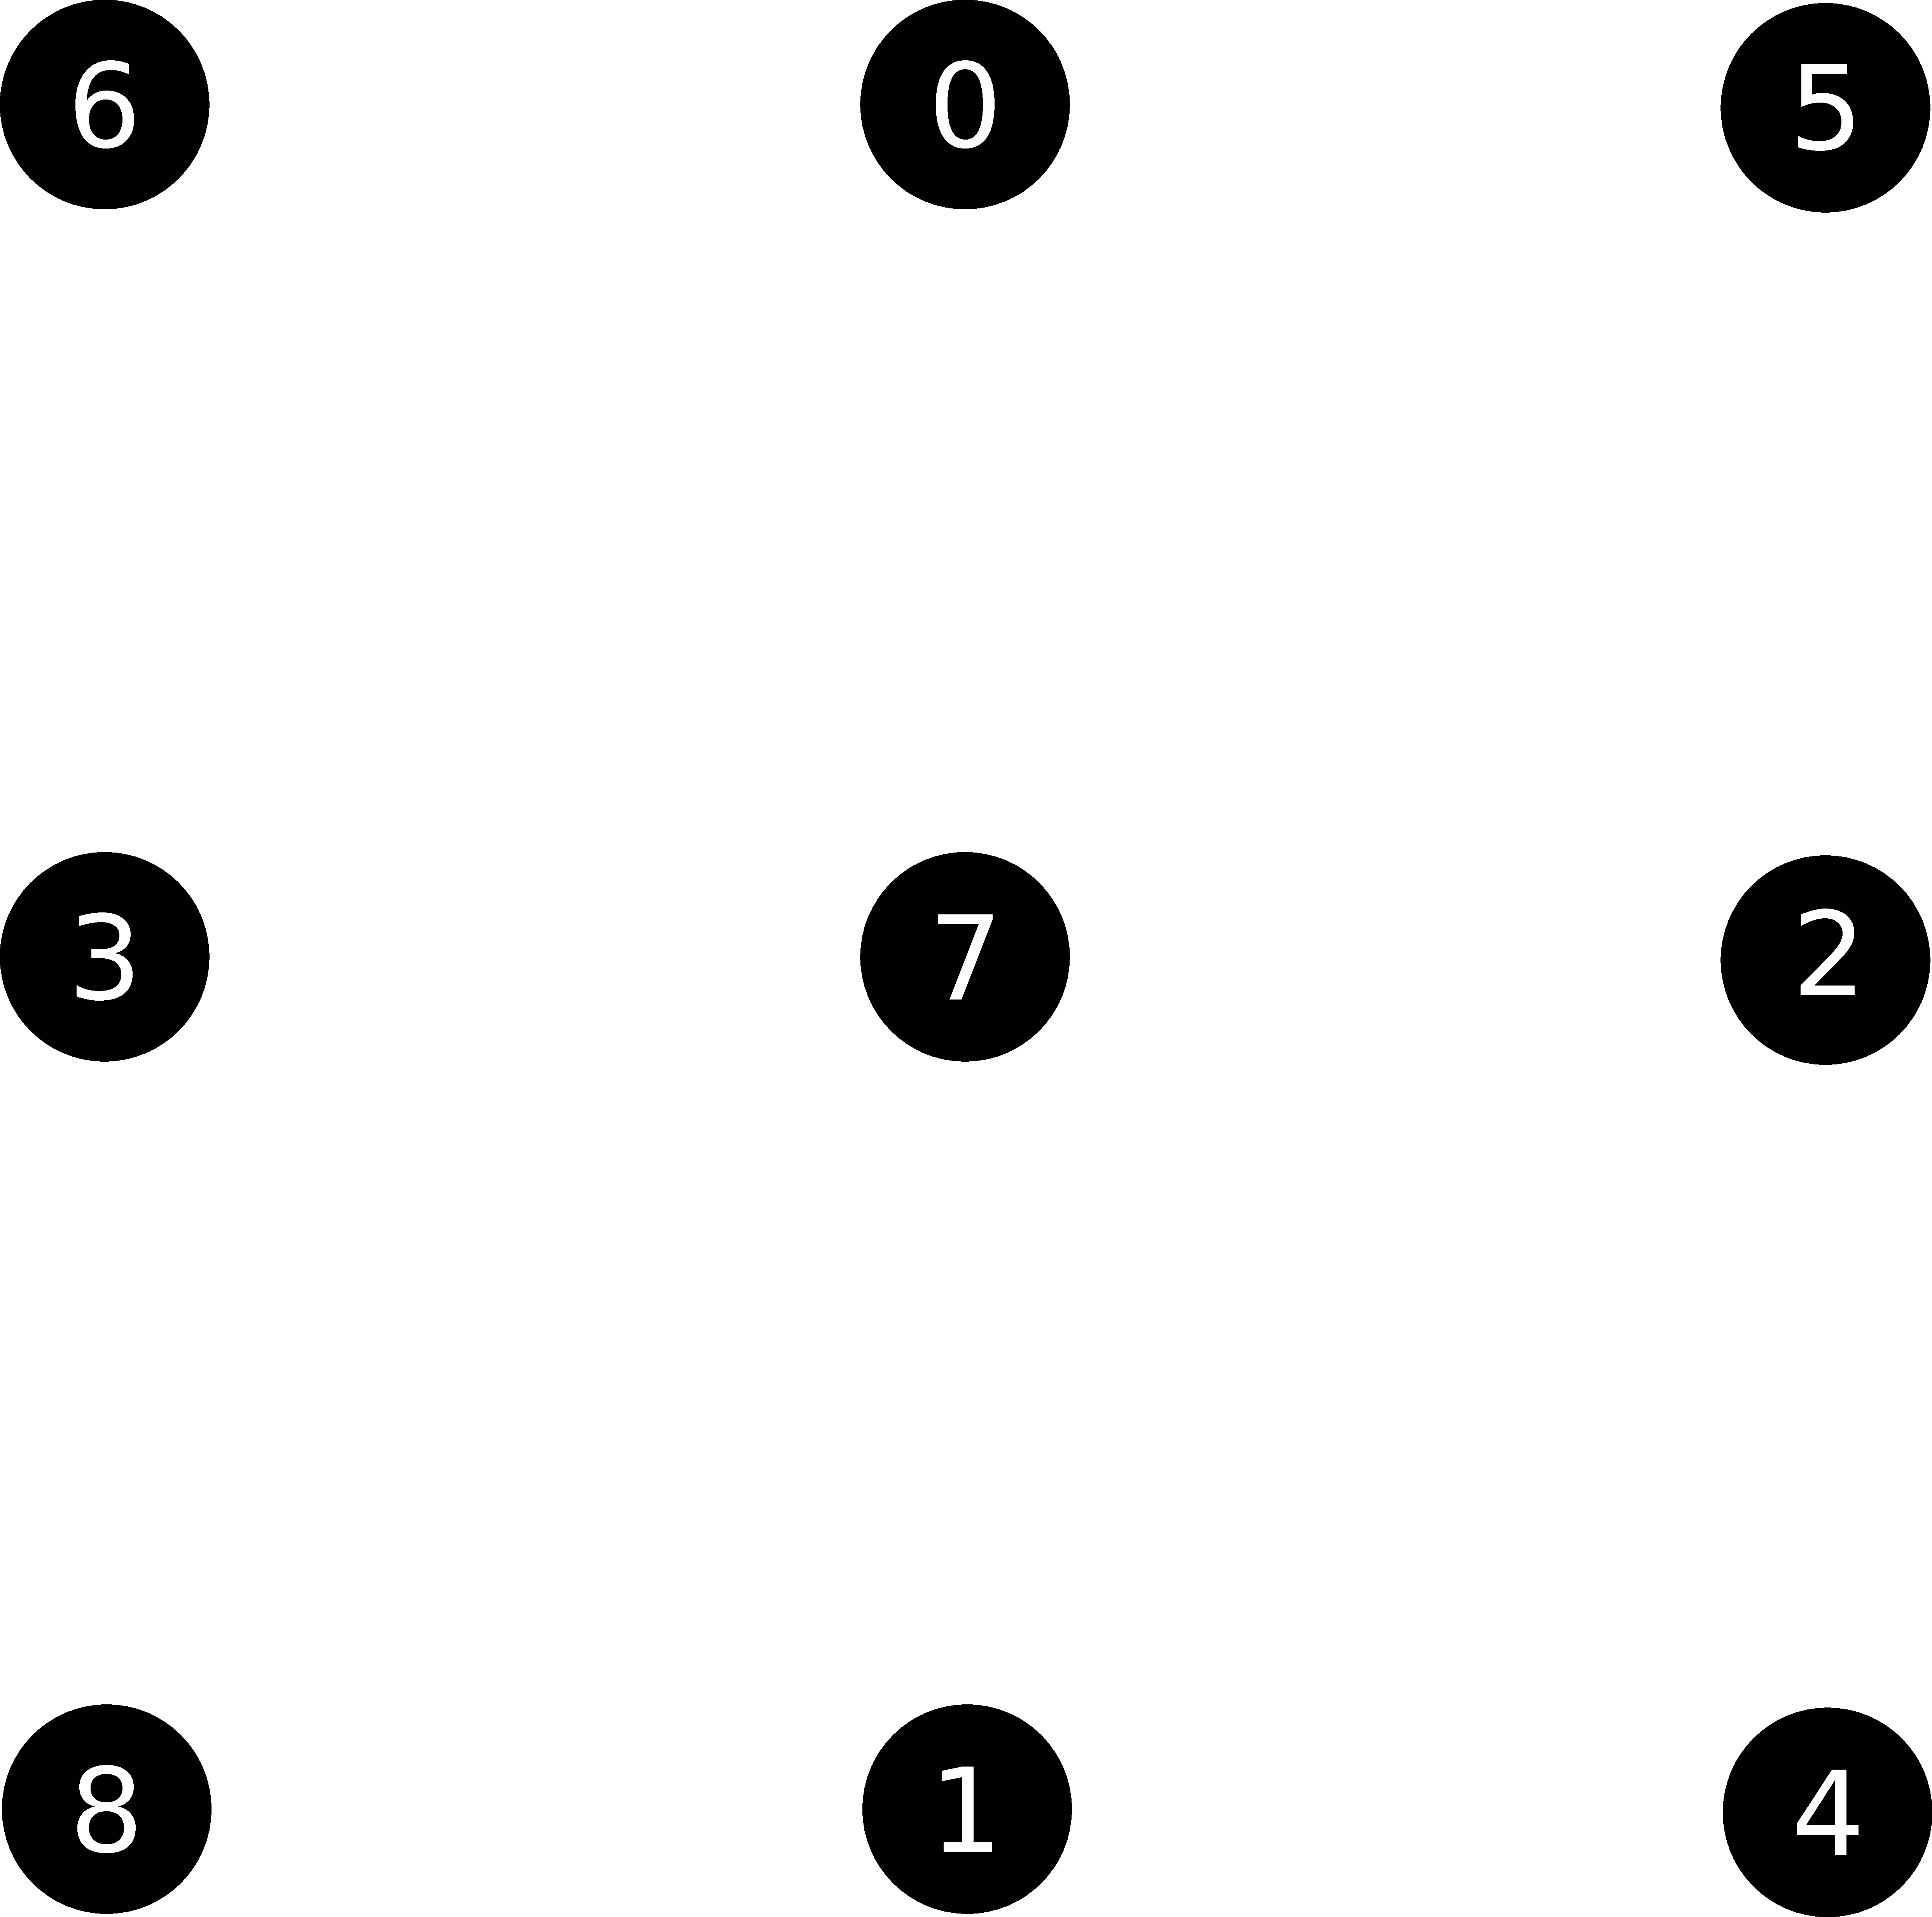
\includegraphics[scale=0.06]{./images/w3x3/w3x3-vertices.pdf}}}%
    \qquad \qquad \qquad
    \subfloat[Simplicial Mesh.]{{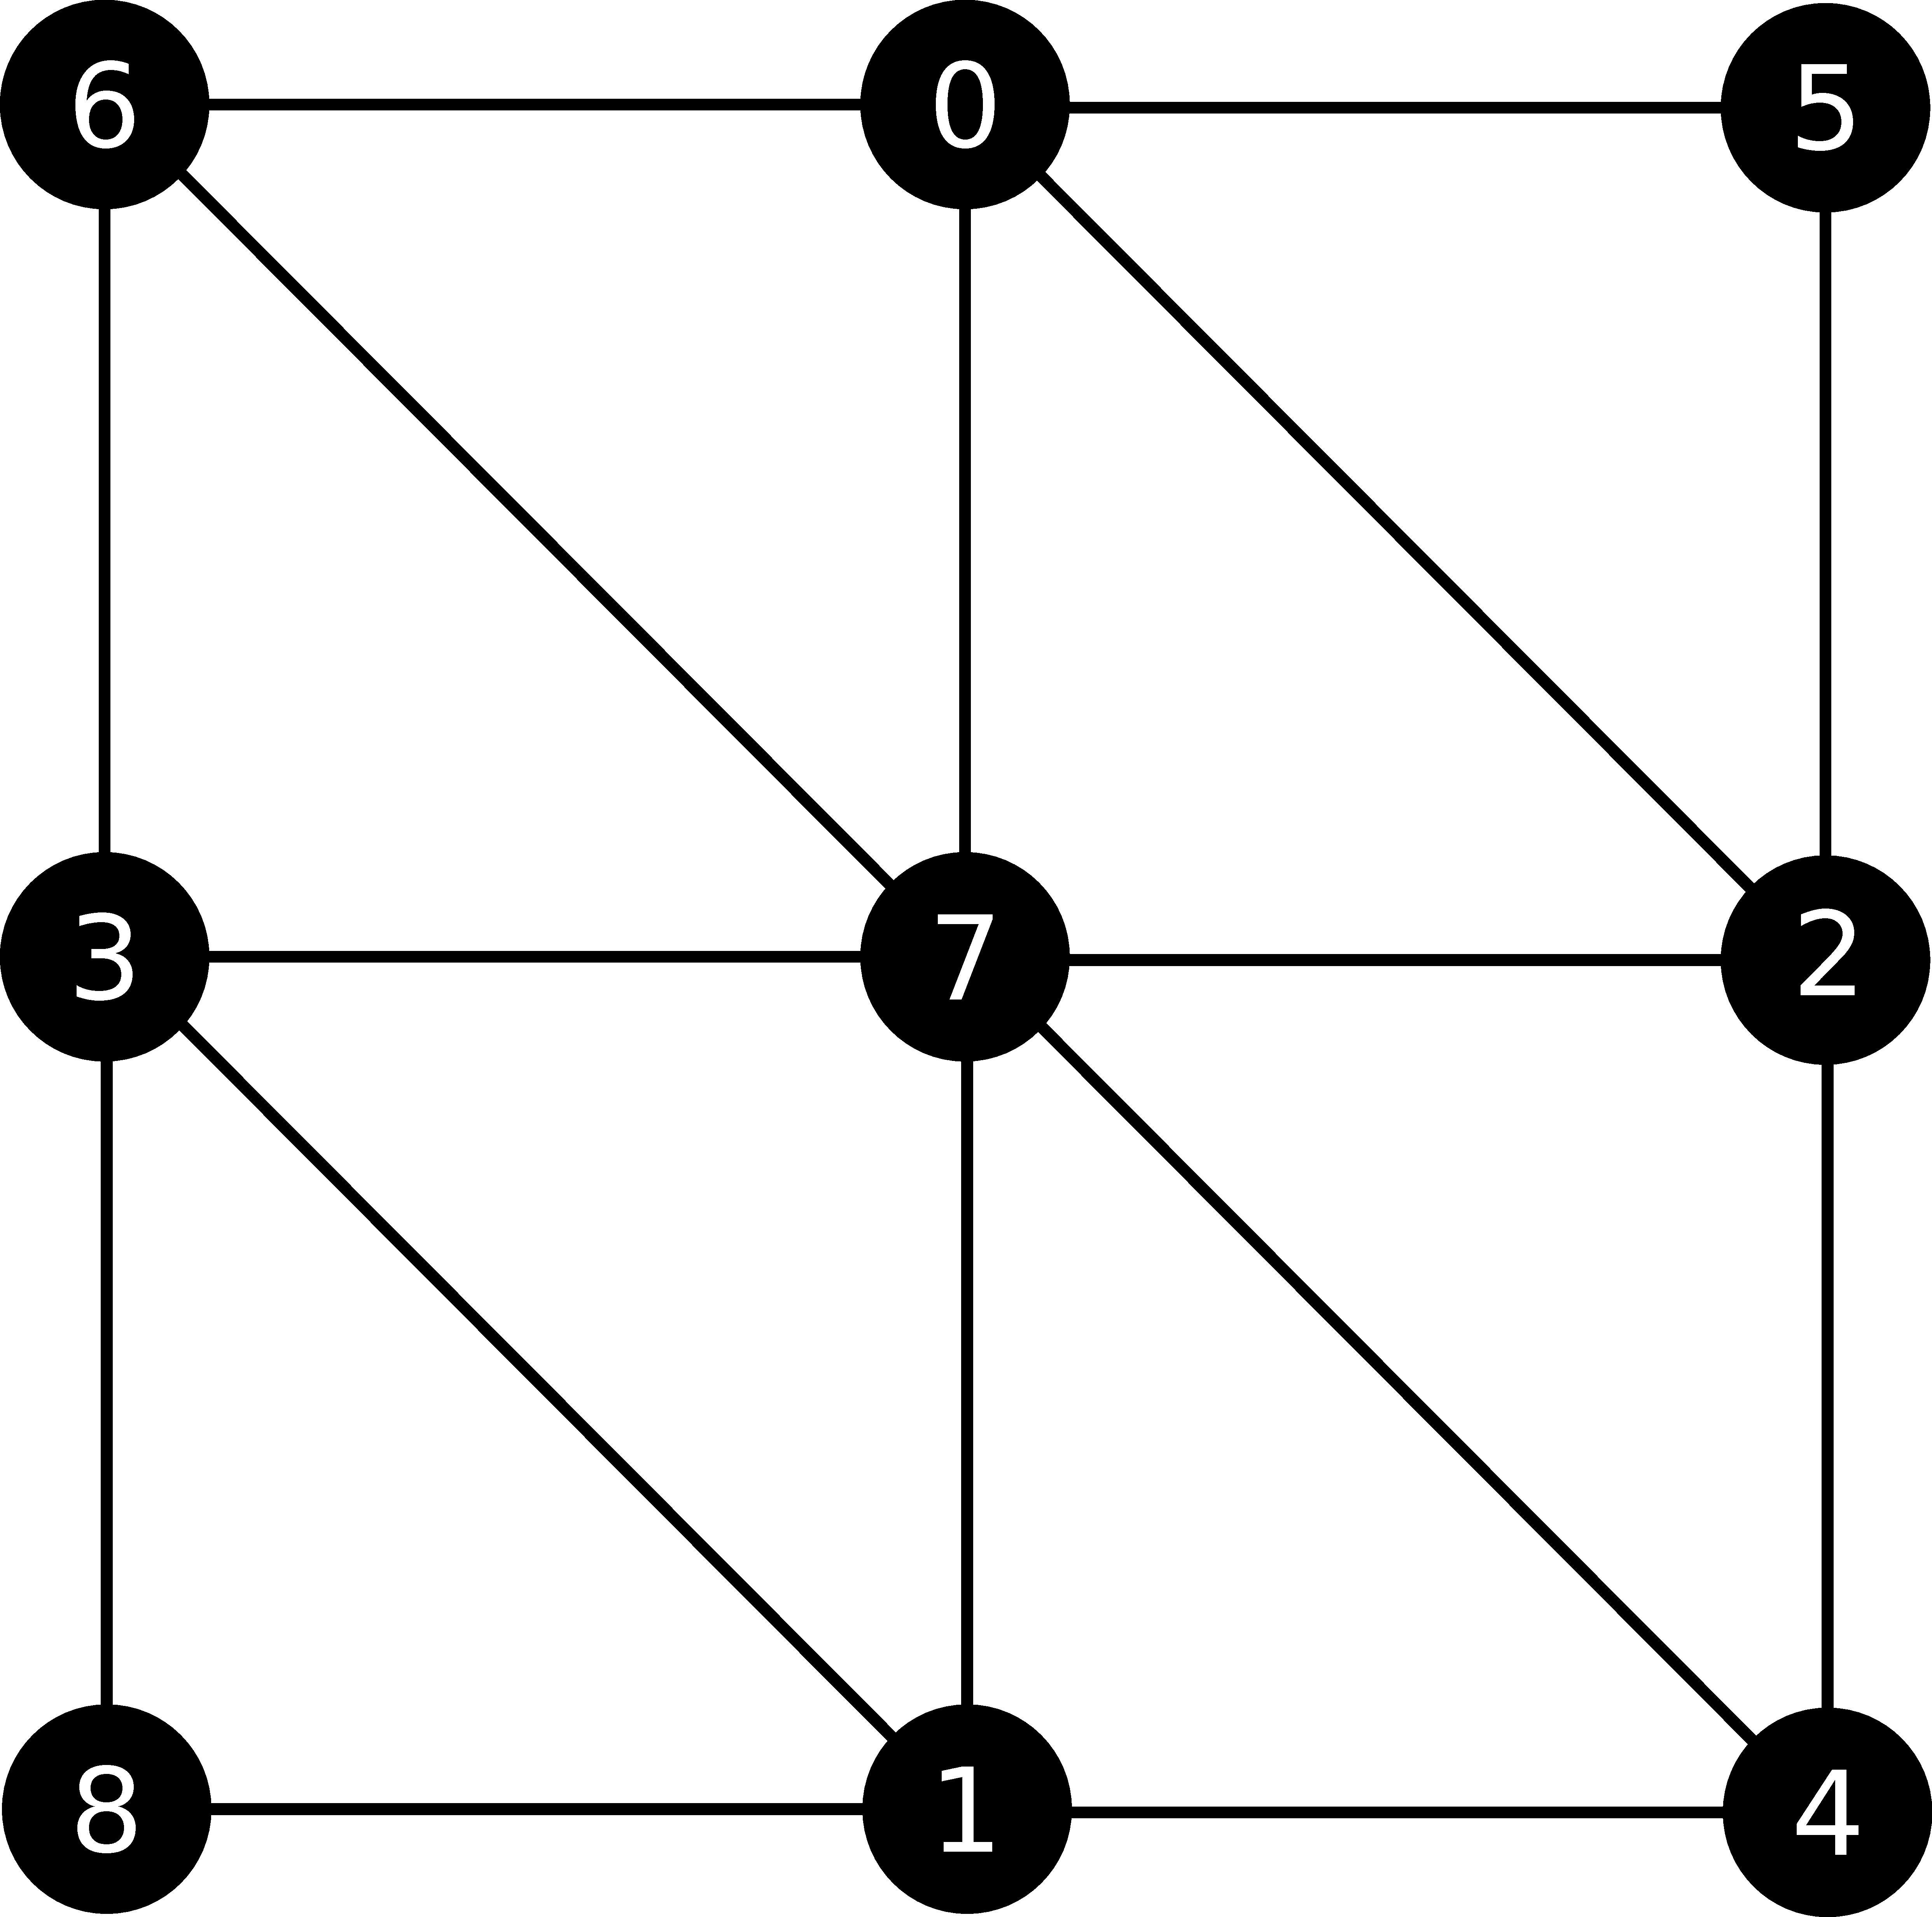
\includegraphics[scale=0.06]{./images/w3x3/w3x3-mesh.pdf}}}%
    \caption{Triangulation of input data to obtain a simplicial mesh.}%
    \label{fig:simplicial-mesh}%
\end{figure}
For simplicity and without loss of generality we will work with two-dimensional domains where the value samples are evenly spaced out in a grid-like fashion (Figure \ref{fig:simplicial-mesh}). The values of the approximation function at the simplicies are obtained via linear interpolation between the vertices of each simplex. As long as the original values we have sampled are unique it can be shown that the linear interpolation function is a Morse function and that all critical points are the vertices of the mesh \cite{curvature-embeded-polyhedra}.

\section{Existing Contour Tree Algorithms}


 % @TODO What about higher dimensions and expand parallel stuff?

The first efficient algorithm for constructing contour trees \cite{first-ct-algo} is due to Van Kreveld et al. Its running time is $O(NlogN)$ on two dimensional domains and $O(N^2)$ in higher dimensions where $N$ is the number of triangles in the simplicial mesh. Tarasov and Vyalyi \cite{second-ct-algo} extended this algorithm to work in time $O(NlogN)$ on three dimensional domains. Their approach however involved a complicated procedure for dealing with multi-saddle points. Both algorithms suffer from lack of generality and non-trivial treatment of multi-saddle points. Carr et. al \cite{ct-big-paper} introduced an algorithm with running time $O(nlogn + N\alpha(N))$ where $n$ is the number of vertices in the simplicial mesh and $\alpha$ is the notoriously slow growing inverse Ackerman function. This algorithm works in any number of dimensions and has simple treatment of multi-saddle points.

More recent developments in the field focus on extending the existing algorithms to accommodate the distributed \cite{distributed-ct-algo, distributed-ct-algo-2} and shared memory parallelism paradigms \cite{parallel-peak-pruning, parallel-ct-1}. The focus of this dissertation will be one of the latest developments in a data parallel shared memory algorithm for contour tree computation
\cite{parallel-peak-pruning}. Before introducing how that algorithm operates and one of the issues related to its parallel performance we will first give a more detailed overview of the most established serial algorithm \cite{ct-big-paper} on which the data parallel one is based on. In order to talk about any of the two algorithms we must establish some notation and define height graphs and trees as they are defined in \cite{carr-masters}.


\section{Height Trees}

A height graph is a graph $G = (V, E)$ together with a real valued function $h$ defined on the vertices of $G$. Height graphs are also known in the literature as weighted graphs. We are changing our notation to be more indicative of the fact that the weight function is defined on the vertices and that it corresponds to height of points in a simplicial mesh. A height tree is a height graph which is a tree. Contour trees are height trees because nodes in the contour tree correspond to nodes in the mesh and can inherit their height (sampled) value. Analogous to the assumption we have made about uniqueness of values we will also assume all vertices in the height trees we consider have unique heights. In other words $h(u) \ne h(v)$ for all $u ,v \in V(G)$ where $u \ne v$. The function $h$ naturally induces a total ordering on the vertices. From now on we will assume the vertices of $G$ are given in ascending order. That is to say, $V(G) = \{v_1, v_2, ... , v_n\}$ where $h(v_1) < h(v_2) < ... < h(v_n)$. This lets us work with the indices of the vertices without having to compare their heights directly. In this notation $h(v_i) < h(v_j)$ when $i < j$.

Introducing the height function allows us to talk about ascending and descending paths. A path in a graph is a sequence of vertices $(u_1, u_2, ... , u_k)$ where $u_i \in V(G)$ for $i \in \{1, 2, ..., k\}$ and $u_iu_{i+1} \in E(G)$ for $i \in \{1, 2, ..., k-1\}$. A path in a height graph is ascending whenever $h(u_1) < h(u_2) < ... < h(u_k)$. If we traverse the path in the opposite direction it would be descending. We will simply call these paths monotone whenever we wish to avoid committing to a specific direction of travel.

When working with height graphs it is useful to extend the definition of a degree of a vertex by taking the height function into account.

\begin{defn} Let $G$ be a height graph and $v$ a vertex of $G$. The up degree of $v$ is defined as the number of neighbours of $v$ with higher value. It is denoted as $\delta^+(v) = \big|\{ u \in N(v) : h(u) > h(v) \}\big|$.   \end{defn}

The down degree of a vertex $v$ is defined analogously as $\delta^-(v) = \big|\{ u \in N(v) : h(u) < h(v) \}\big|$. In the context of height trees the definitions of up and down degrees of a vertex allow us distinguish between two types of leaves - lower and upper leaves.
\begin{defn} Let $G$ be a height graph and $v$ a vertex of $G$. If  $\delta^+(v) = 1$ and $\delta^-(v) = 0$ then $v$ is a lower leaf.  \end{defn}

If $\delta^+(v) = 0$ and $\delta^-(v) = 1$ then $v$ is an upper leaf. We will see in the next section how differentiating between the two types of leaves is a critical part in the computation of the contour tree.

\section{Serial Algorithm}

The contour tree is a tree that consists of \cite{first-ct-algo}:

\begin{itemize}
    \item Vertices or supernodes that correspond to level sets that contain a critical point.
    \item Edges or superarcs correspond to path-connected regions bounded by two level sets which both contain a critical point. They connect the supernodes those level sets correspond to.
\end{itemize}

% @TODO Think about this contruction and destruction business
The contour tree contains information of two types of events - joining and splitting of contours. We can derive two other height trees from the contour tree that each contain the information of the joining and splitting events separately. These are called the join and split trees \cite{ct-big-paper}. The join tree contains information for the contours that join together and the split tree holds the information for the contours that split apart. The join tree of a contour tree summarises the evolution of the connectivity of the sublevel sets of the interpolation function and the split tree of the superlevel sets. You can find an example of the join and split trees of Figure \ref{fig:mesh-join-split-contour}.

% The two are symmetric in that the join tree of the function $f$ is isomorphic to the split tree of the negative of the function $-f$.

\begin{figure}[h]%
    \centering
    \subfloat[Simplicial mesh.]{{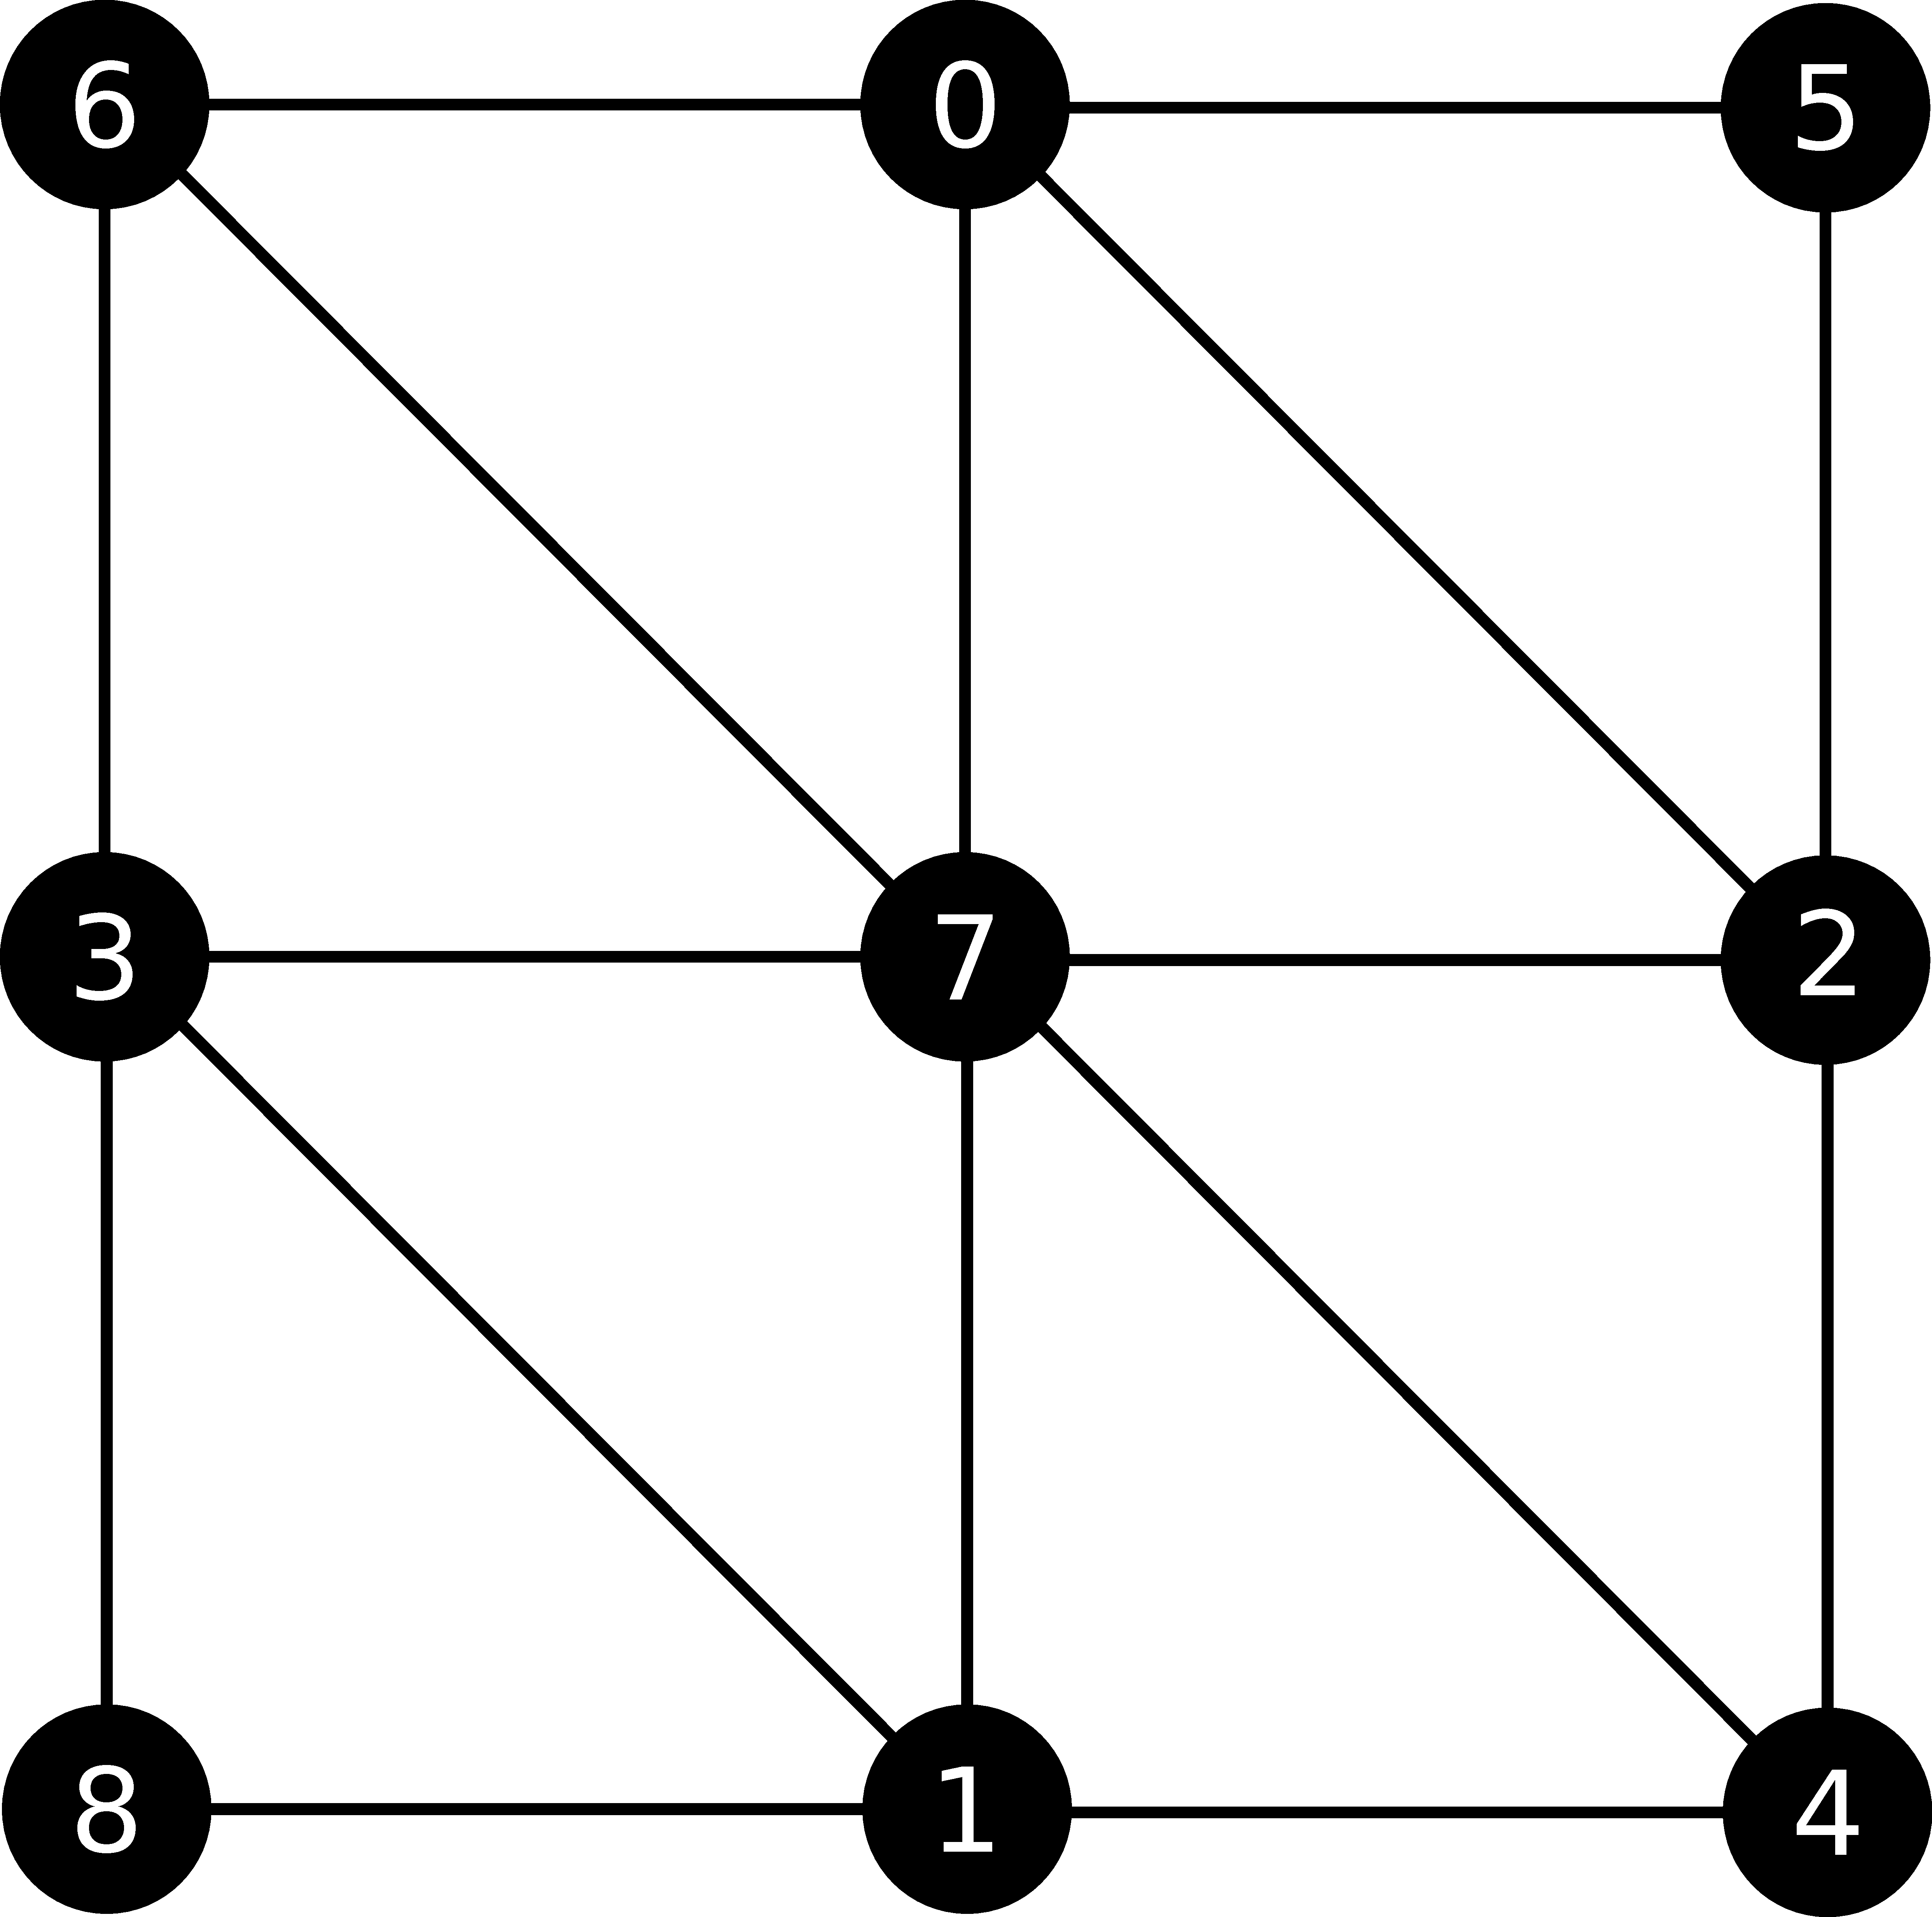
\includegraphics[scale=0.06]{./images/filtration/asc/x9.pdf}}}%
    \qquad \qquad \qquad
    \subfloat[Contour tree.]{{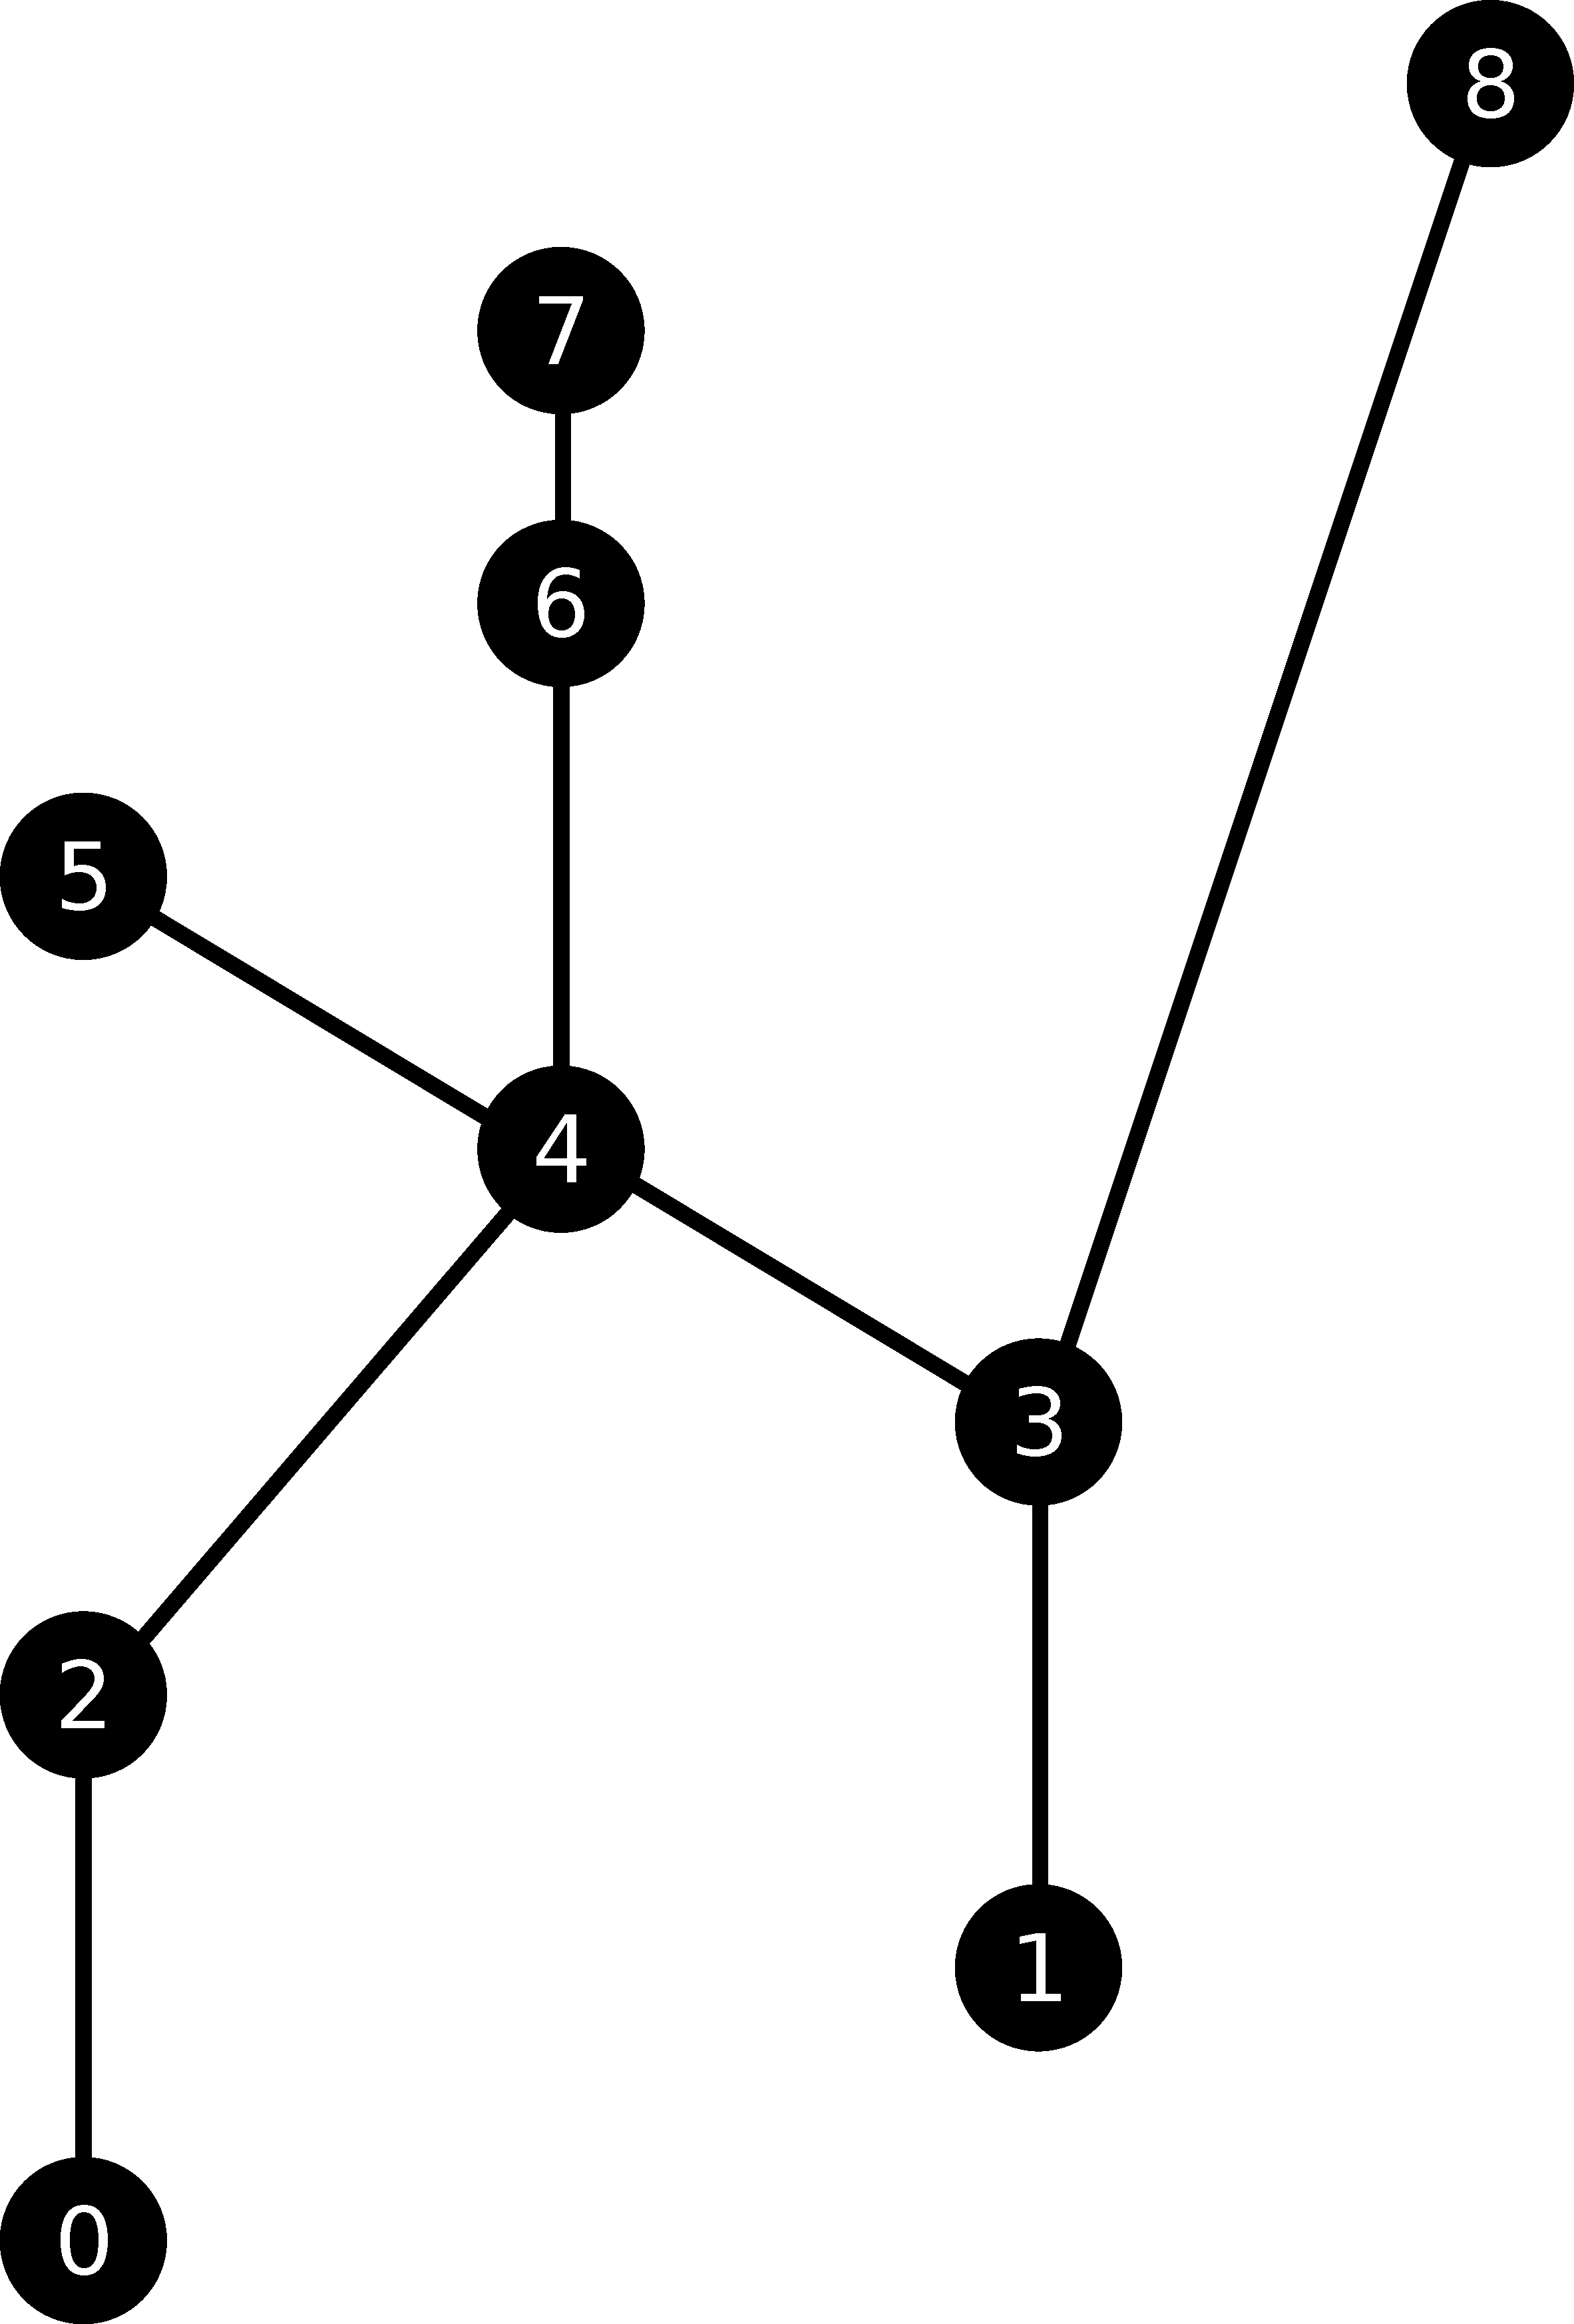
\includegraphics[scale=0.10]{./images/w3x3/w3x3-contour-tree.pdf}}}%
    \qquad \qquad \qquad

    \subfloat[Join tree.]{{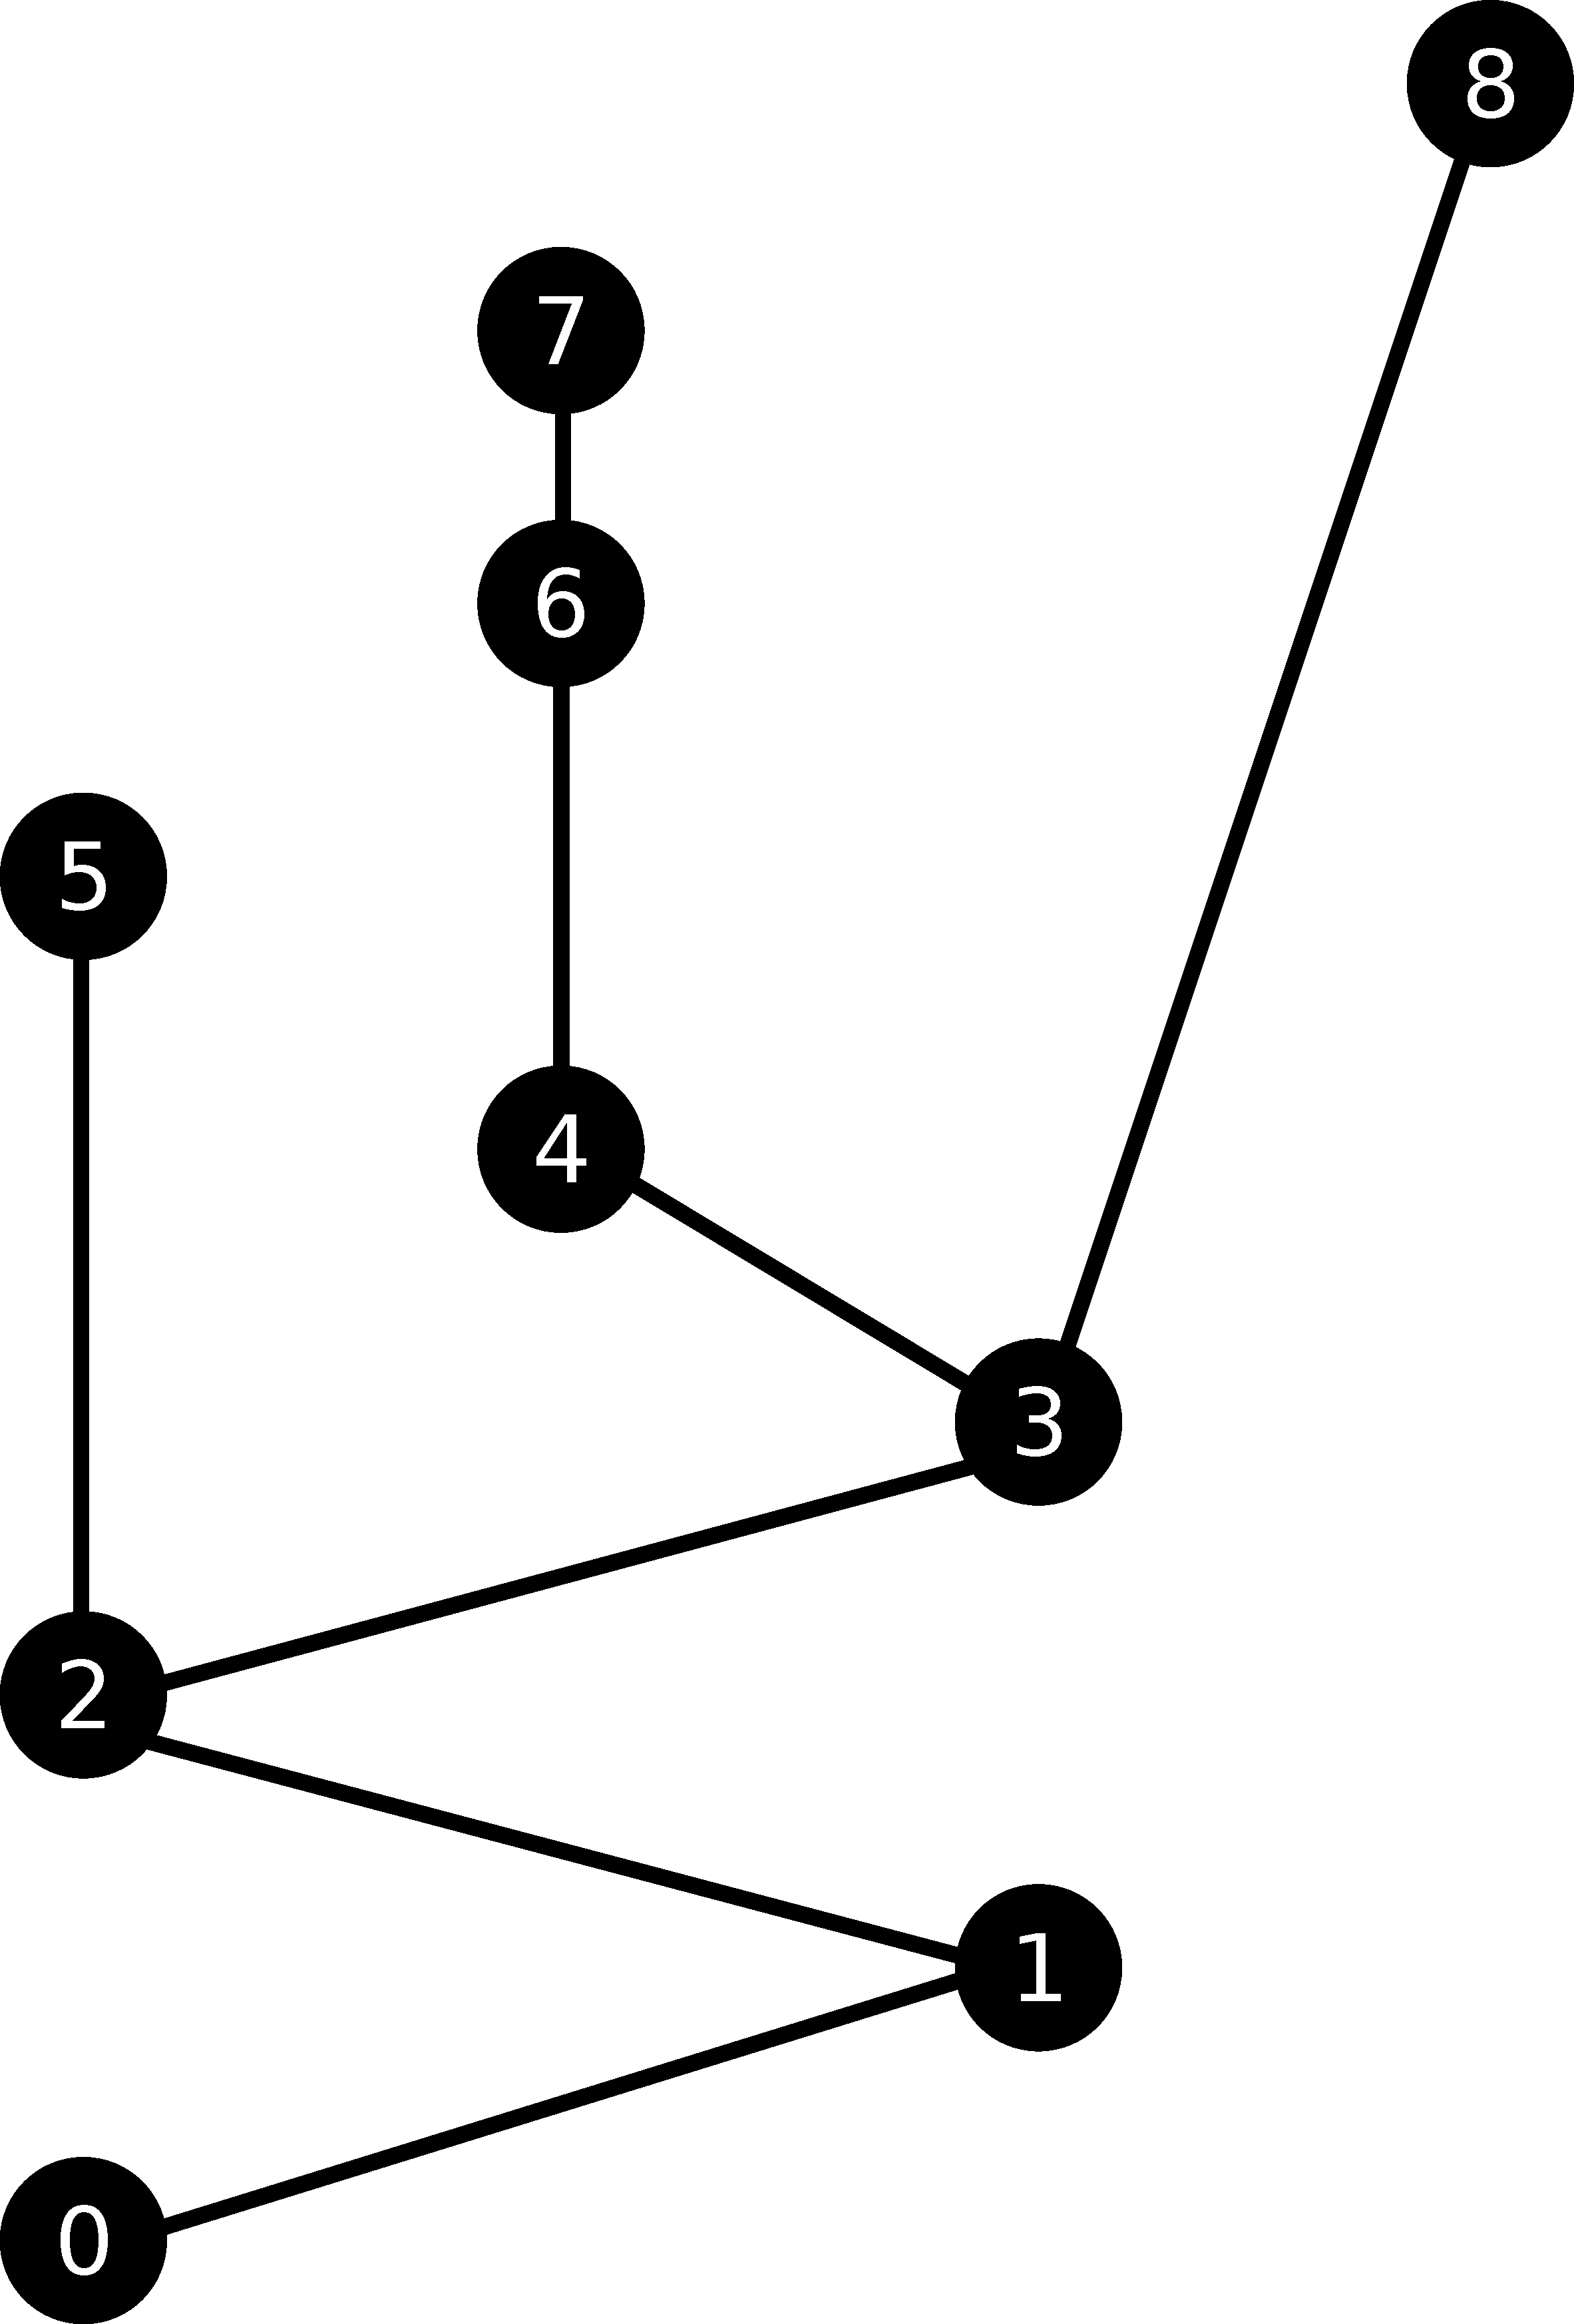
\includegraphics[scale=0.10]{./images/w3x3/w3x3-join-tree.pdf}}}%
    \qquad \qquad \qquad
    \subfloat[Split tree.]{{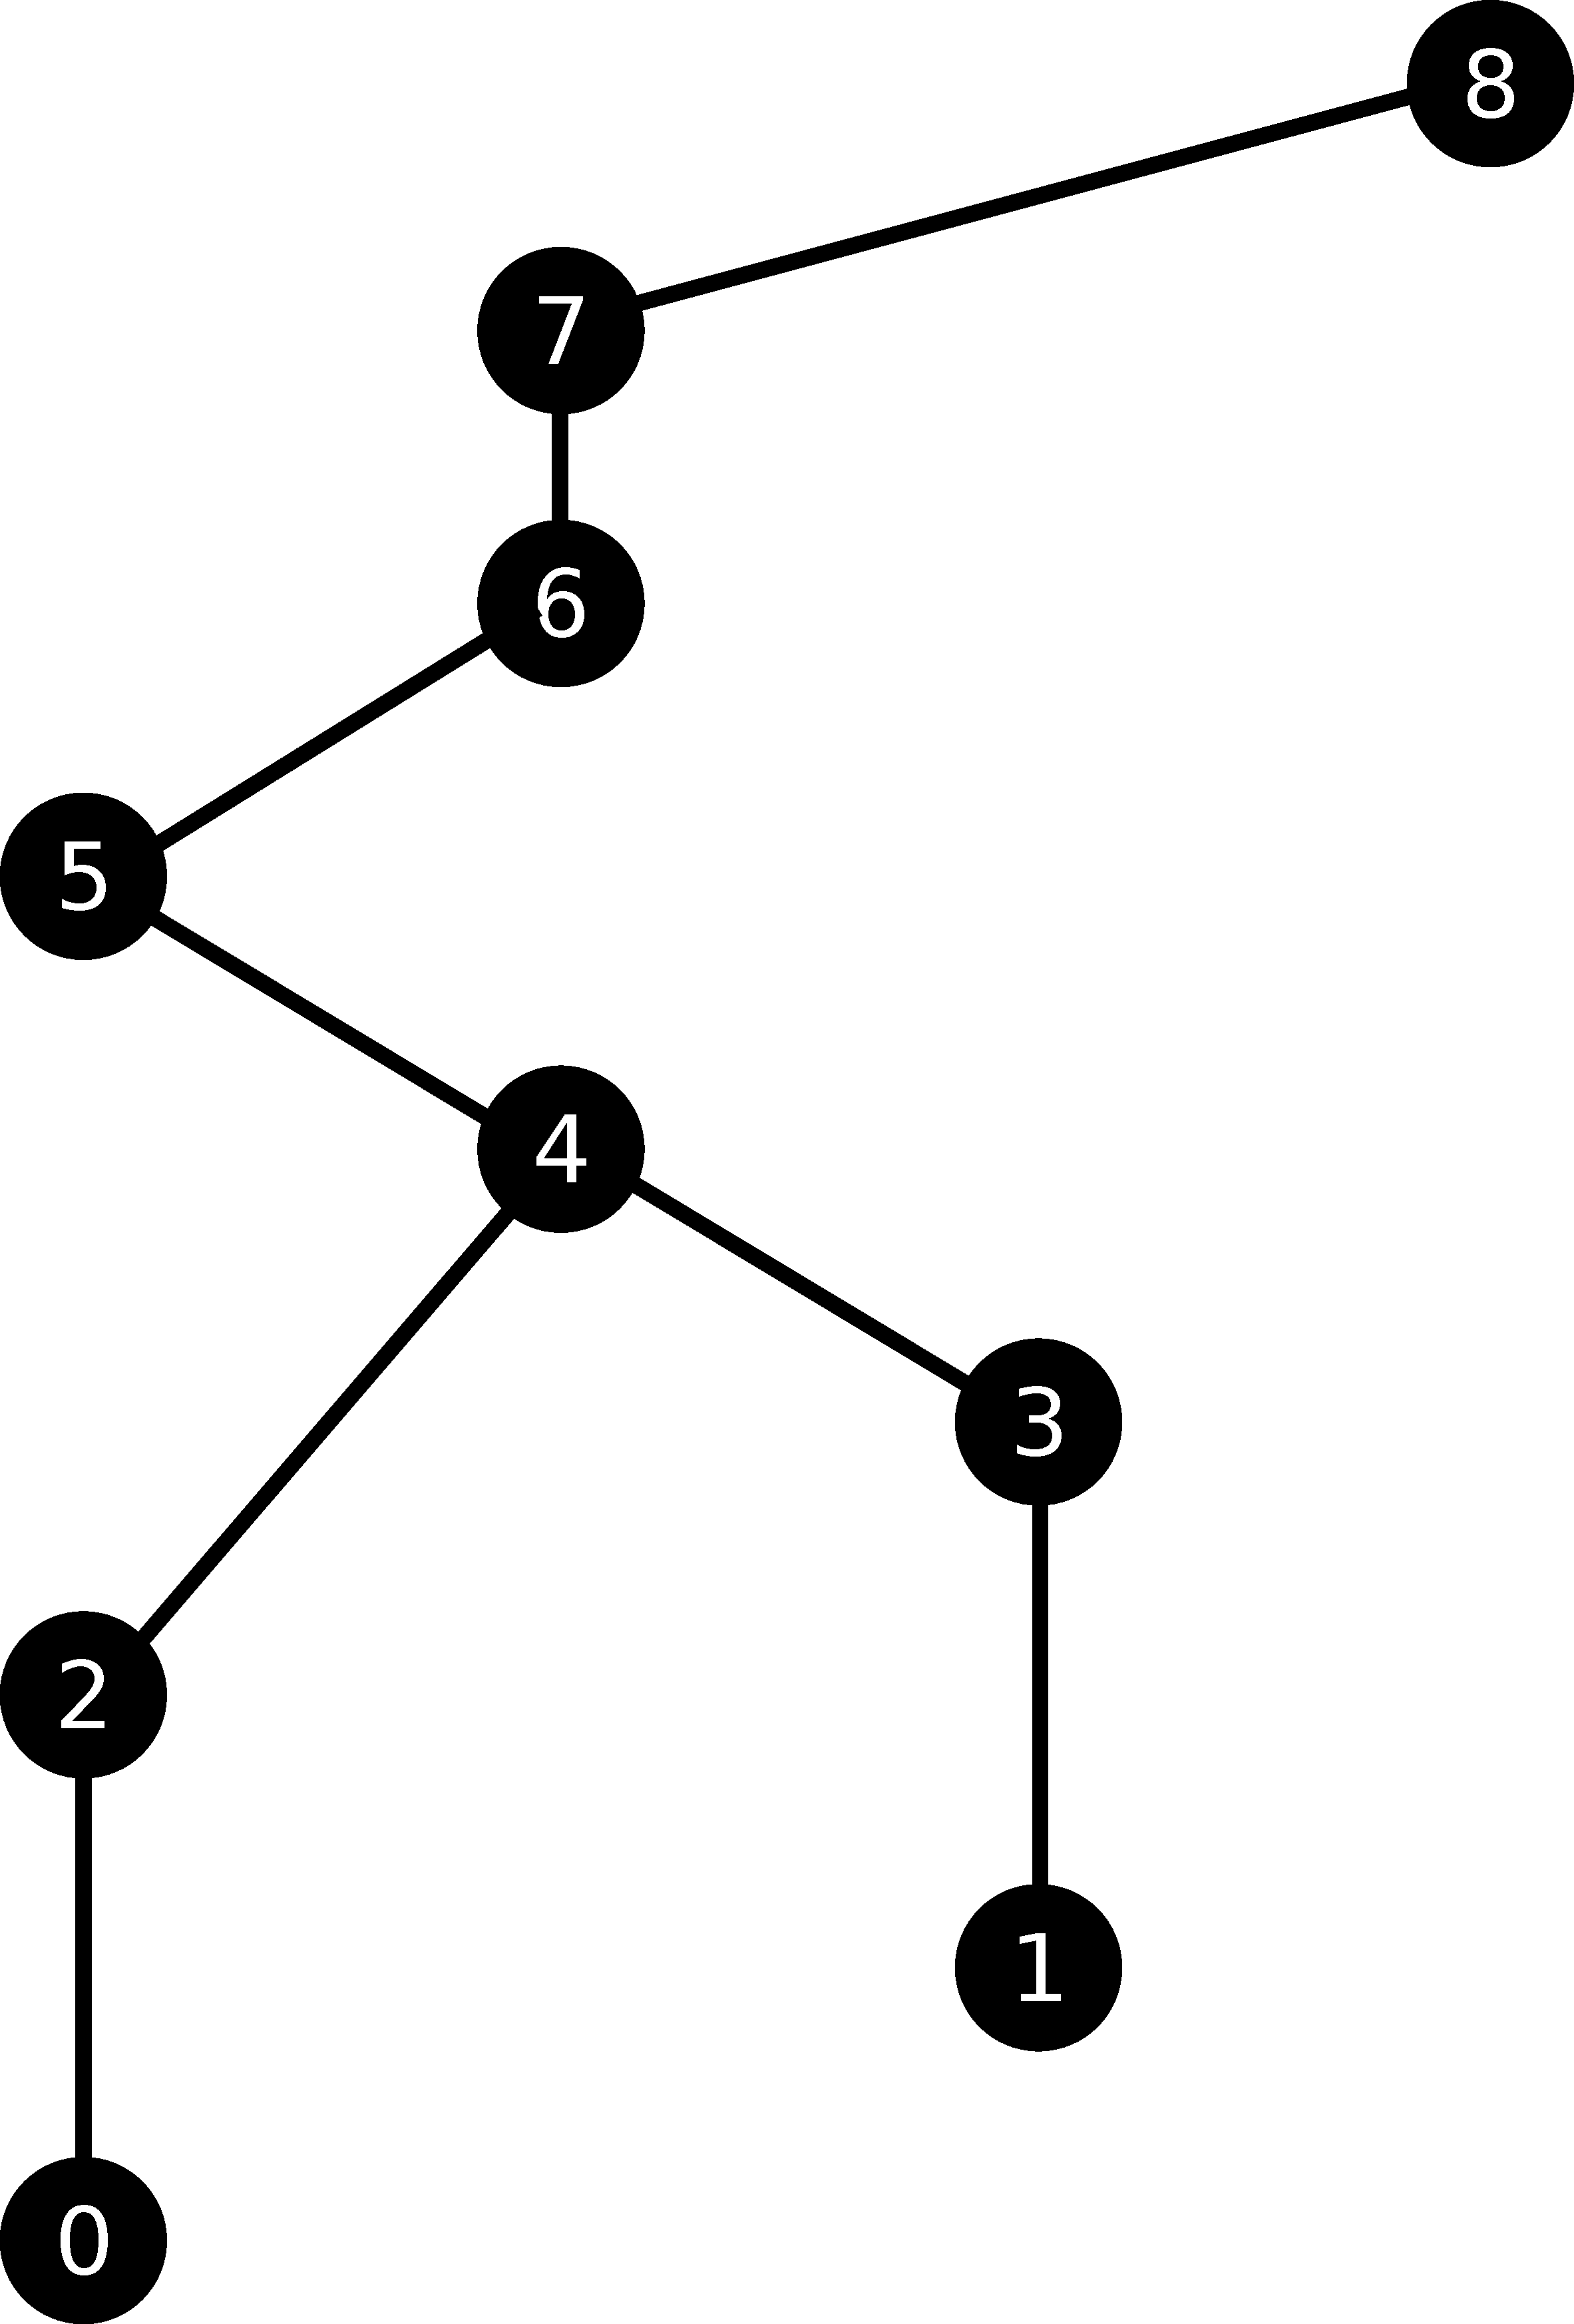
\includegraphics[scale=0.10]{./images/w3x3/w3x3-split-tree.pdf}}}%
    \caption{The simplicial mesh, join and split trees and contour tree.}%
    \label{fig:mesh-join-split-contour}%
\end{figure}

The reason we would like to study join and split trees is that the contour tree can be reconstructed from them. The core idea of the algorithm we will present is that we can derive the join and split trees directly from the simplicial mesh and then combine them to obtain the contour tree. We will first describe how the join and split trees are computed from the mesh. We only have to describe the process for the join tree because the computation of the split tree is symmetrical \cite{ct-big-paper}.

\begin{defn} A join component is a connected component in the superlevel set $f^{-1}([h, \infty))$ at some $h \in \mathbb{R}$.  \end{defn}

Let $M$ be the simplicial mesh from Figure \ref{fig:mesh-join-split-contour} (a) and let $h : M \to \mathbb{R}$ be the interpolation function defined on it. We will refer to $h$ as the height function. To construct the join tree we are going to have to keep track of which components merge together in the superlevel sets of $h$. We will consider all superlevel sets $M^t = h^{-1}([t, \infty)) = \{x \in M : h(x) \in [t, \infty) \}$ as a one parameter family $\{M^t\}_{t \in \mathbb{R}}$
of nested subsets of $M$. We can see from this definition that $M^a \subseteq M^b$ whenever $a \le b$. What the join tree captures is how the connectivity of the superlevel sets changes as the parameter $t$ is increased. The connectivity of superlevel sets changes either at local minima where a new component is created or a saddle point that merges two or more join components.

%We will not formalise the notion of tracking join components and constructing a join tree. Let us work in the general setting where $X$ is any path-connected topological space and $h : X \to \mathbb{R}$ is a function defined on $X$. The claims we make will hold in the special case where $X$ is a simplicial complex. Let us consider all sublevel sets $X_t = h^{-1}((-\infty, t]) = \{x \in X : h(x) \in (-\infty, t] \}$. They form a one parameter family $\{X_t\}_{t \in \mathbb{R}}$ of nested subsets where $X_a \subseteq X_b$ whenever $a \le b$. What the join tree captures is how the connectivity of the sublevel sets changes as the parameter $t$ is increased.

To visualise this process we can contract every join component to a point much like we did in the Reeb graph. The only difference here is that the equivalence relation is defined for all points in a superlevel set $h^{-1}([t, \infty))$ instead of a level set $h^{-1}(\{t\})$. Because of this change and because join components can only merge the join tree is a tree \cite{comp-topo}. Furthermore if $M_m = M$ is the last superlevel set for some $m \in \mathbb{R}$ then all join components merge into one because $M$ is path connected.

We will briefly outline the algorithm for constructing the join tree and refer the reader to \cite{ct-big-paper} for further implementational details. We know that all critical points are vertices of $M$ and that it is only at the critical points that changes in the topology of the superlevel sets can happen. The algorithm works by considering the vertices of the simplicial mesh in ascending order of their height. If the current vertex is a local minimum we directly add it in the join tree because it starts a join component. If the current vertex is a saddle that joins two or more components (join saddle) we add it to the join tree and add an edge between it and the local minima of the join components it merges. At the end of the computation all vertices will be in the same join component. In order to keep track of which join components different vertices belong to we can use the union-find data structure. The term  $\alpha(n)$ in the time complexity of the contour tree algorithm comes from the basic operations of find and search in the union-find data structure.

% @TODO Define Join Saddles and Subdivided edges
Not all vertices of the mesh will be in the join tree. Only those which correspond to local maxima and to join saddles. This will pose a problem later on when we wish to combine the join and split trees. To avoid this problem we can augment the join tree by adding all missing vertices. This is done through edge subdivision. Let $a \text{ and } b$ be two adjacent vertices in the join tree.  Let $\{v_1, v_2, ..., v_n\}$ be vertices in the mesh that are not in the join tree that are given in ascending order in terms of height.  Suppose that $h(a) < h(v_i) < h(b)$ for all $i \in \{1, 2, ..., n\}$ and the vertices $v_i$ are in the same connected component of $X_b - h^{-1}(\{b\}) = h^{-1}((-\infty, b))$. In order to augment the join tree with the first vertex we subdivide the edge $ab$ and label the new vertex as $v_1$. Next we subdivide $v_1b$ and label the new vertex as $v_2$. We continue to do so and on the $k$th step we subdivide the edge
$ v_{k-1}b $ and label the new vertex as $v_k$  .

The procedure of augmentation can be applied to the split tree and contour tree as well. We can use it to augment the contour tree with all vertices of the mesh which are not critical points. This is why we will differentiate between the contour tree and the augmented contour tree. The augmented contour tree contains all regular vertices of the simplicial mesh.

The second step of the algorithm is to combine the join and split trees to produce the contour tree. We will actually combine the augmented join tree with the augmented split tree to obtain the augmented contour tree. Removing the augmentation of the contour tree is left as an optional final step. The first step in merging the two is to identify all leaves of the contour tree and their incident edges. We can recognize them immediately from the join and split trees using the following property \cite{carr-masters}.

\begin{property} Let $v$ be a vertex such that its up degree in the join tree is $0$, its down degree in the split tree is $1$ and $u$ is its only down neighbour in the split tree. Then $v$ is an up leaf in the contour tree and $vu$ is an edge in the contour tree.  \end{property}

There is an analogous property in the case of down leaves and their adjacent edges.

\begin{property} Let $v$ be a vertex such that its up degree in the join tree is $1$, its down degree in the split tree is $0$ and $u$ is its only down neighbour in the join tree. Then $v$ is a down leaf in the contour tree and $vu$ is an edge in the contour tree.  \end{property}

Now suppose that we have identified $v$ as a leaf and $vu$ as its adjacent edge in the split or join tree. Another property \cite{carr-masters} tells us that if we perform vertex contraction on $v$ (remove $v$ and form a clique from its neighbourhood) from the join, split and contour trees we obtain the join and split trees of the contour tree with $v$ removed. This allows us to iteratively remove leaves from the join and split trees, add them to the contour tree and then delete them from the join and split tree. We can repeat this process until we have removed all vertices from the join and split trees and all vertices are present in the contour tree. For a detailed description of this process we refer the reader to \cite{ct-big-paper}.

 % We are allowed to do so because removing all leaves in a tree leaves the tree with at least one leaf if it is not empty where the algorithm will terminate.

The Serial algorithm for the construction of the contour tree is a summary of the results we have obtained so far:

\textbf{Step 1.} Read input data and convert it to a simplicial mesh.

\textbf{Step 2.} Compute the augmented join and split trees from the simplicial mesh.

\textbf{Step 3.} Iteratively remove leaves from the augmented join and split trees and add them to the augmented contour tree until the augmented join and split trees are empty.

\textbf{Step 4.} Remove regular vertices from the augmented contour tree by contracting them.

\section{Parallel Algorithm}

The data parallel contour tree algorithm \cite{parallel-peak-pruning} is largely based on the serial contour tree algorithm we just described. The parallel approach borrows the two phase methodology of computing the join and split trees and then merging them. We will omit describing the process of parallelising join/split tree computation because it is not directly related to the issue we aim to address. We will describe how the merge phase is parallelised in detail.

The data-parallel paradigm works best when there are a large number of computational tasks to be carried out independently. Dependant tasks require some form of synchronisation. Synchronisation is costly in terms of performance. Removing a leaf in the merge phase of the serial algorithm requires little synchronisation with other vertices because it is a local operation. It only involves a few of the vertices of the join and split trees. This means that once we identify all up and down leaves we can remove them in parallel in a single iteration. The key problem to solve in the merge phase is to reduce the number of total iterations needed to remove all vertices from the join and split trees. The amount of parallelism in this computation is limited by the number of leaves at each iteration. For example a tree which is a path of length $n$ will take at least $n/2$ iterations and a tree with one central vertex and $n$ leaves adjacent to it will take only two iterations.

In a graph with no vertices of degree two at least half of the vertices are leaves (see Appendix \ref{chapter-proofs}). If at every iteration half of the remaining vertices are leaves the total number of iterations would be logarithmic in the number of vertices in the contour tree. In order to ensure this logarithmic collapse Carr et. al \cite{parallel-peak-pruning} have come up with a way of batching some of the paths that start at a leaf and consist of vertices of degree two, in a single iteration. We will call such paths leaf chains. The process of removing them in a single iteration is in effect equivalent to contracting all vertices in the tree of degree two. This leaves only leaves and vertices of degree three or higher and ensures the logarithmic collapse.

The main issue that arises is that leaf chains which are not monotone paths canno be processed in a single iteration. They require multiple iterations to process. When some of the vertices in the leaf chains have alternating height and we plot them according to their height they form a characteristic zigzag pattern. We will call paths W-Structures. See for example the path $(5, 2, 4, 3, 8)$ in the contour tree on Figure \ref{fig:mesh-join-split-contour}. These w-structures are the core issue we are addressing in this dissertation. We would like to obtain a better understanding of them and how and why they affect computation. The first step to solving such a problem is understanding it. The next chapter will address this by developing algorithms that analyse contour trees and determine the largest w-structures that is present in them.

% The issue arises from batching monotone paths is not a monotone path and some of the vertices inside it have alternating height. The we can only batch monotone subpaths and not the whole path. The more zig zags there are in the path the less monotone paths there and the more iterations we will require. This effectively serialises computation along them.

The theoretical issue caused by the w-structures becomes evident in the algorithmic analysis of the parallel contour tree algorithm. According to that the key question in the merge phase of the algorithm is how many iterations are needed to collapse the contour tree. Each iteration takes $O(1)$ steps, because all leaves can be processed in parallel, and $O(t)$ work, where $t$ is the number of leaves. This leads to an overall complexity of $O(log(t))$ steps and $O(tlog^2(t)$ work if we assume that no w-structures are present. If however there is a w-structure with more zigzags than $log(t)$ then the authors of the paper claim that the best formal guarantee they can give for the steps is the diameter of the contour tree. One of our goals in analysing the w-structures is to provide a better bound than the diameter of the tree. We will demonstrate how this can be done by developing some new theory about the w-structures in Chapter 4 and through an empirical analysis in Chapter 7.


\section{Contour Tree Simplification}

Finally we will introduce the topic of contour tree simplification. A central problem in using contour trees in visualisation is simplifying their output and presenting only the most important parts to enable human comprehension. The complexity of a contour tree of a large enough data set could severely limit its use. This is why it is vital to employ techniques that simplify the contour trees by removing parts of them that correspond to less "significant" topological features or sampling noise and error. This process helps to reveal the fundamental topological structures present in data.

% The most recent extensions of this work introduce high quality topological simplification [4] where the contour tree is pruned incrementally to reduce its complexity and highlight the fundamental structures present in the data.

% @TODO Add hamish phd thesis as generalisation?

One technique for contour tree simplification is branch decomposition \cite{ct-branch-decomp}. Branch decomposition involves decomposing the contour tree into a set of edge-wise disjoint monotone paths (branches) which cover all edges of the tree. The trivial branch decomposition of any tree is obtained by taking every edge to be a separate branch. A branch decomposition is hierarchical when there is exactly one branch that connects two leaves and every other branch connects a leaf to an interior node. An example of a hierarchical branch decomposition is shown in Figure \ref{fig:branch-decomp}.

The branches in this scheme represent pairs of critical points. This pairing of critical points forms the basis for a topological simplification. The topological simplification consists of removing branches that do not disconnect the tree. This produces a hierarchy of cancellations like in Figure \ref{fig:branch-decomp}. We define the persistence of a branch to be the bigger of the difference between its end points and the persistence of its children. Branches of high persistence reflect more prominent features in the tree. We apply the simplification by removing branches with low persistence that do not disconnect the tree.

The algorithm for producing the hierarchical branch decomposition of a contour tree is the following:

\begin{itemize}
    \item Identify all upper leaves that connect via branches to upwards saddles (merging of components).
    \item Identify all lower leaves that connect via branches to downwards saddles (splitting of components).
    \item Those pairs of leaves and saddles are the candidate branches. We pick the one with the lowest persistence (difference of height between the leaf and the saddle).
    \item Remove all vertices in the branch without the saddle.
    \item Continue this process until a single branch that connects two leaves is all that remains. That is the root branch.
\end{itemize}

For example let us construct the hierarchical branch decomposition of the contour tree from Figure \ref{fig:mesh-join-split-contour}. The first two candidate branches we identify are $(5, 2)$ with persistence $3$ and $(3, 8)$ with persistence $5$. We take the branch with lower persistence $(5, 2)$. In the next step the candidate branches are $(0, 4)$ with persistence $4$ and $(3, 8)$ with persistence $5$. We will take $(0, 4)$.
Afterwards the remaining candidate branches are $(3, 7)$ with persistence $4$ and $(3, 8)$ with persistence $5$. After removing $(3, 7)$ in the final stage the only remaining branch is $(1, 8)$. It is the root branch because it connects two leaves.
The produced pairs of critical points are $(2, 5), (0, 4), (3, 7)$ and $(1,8)$.

\begin{figure}%
    \centering
    \subfloat[Branch decomposition.]{{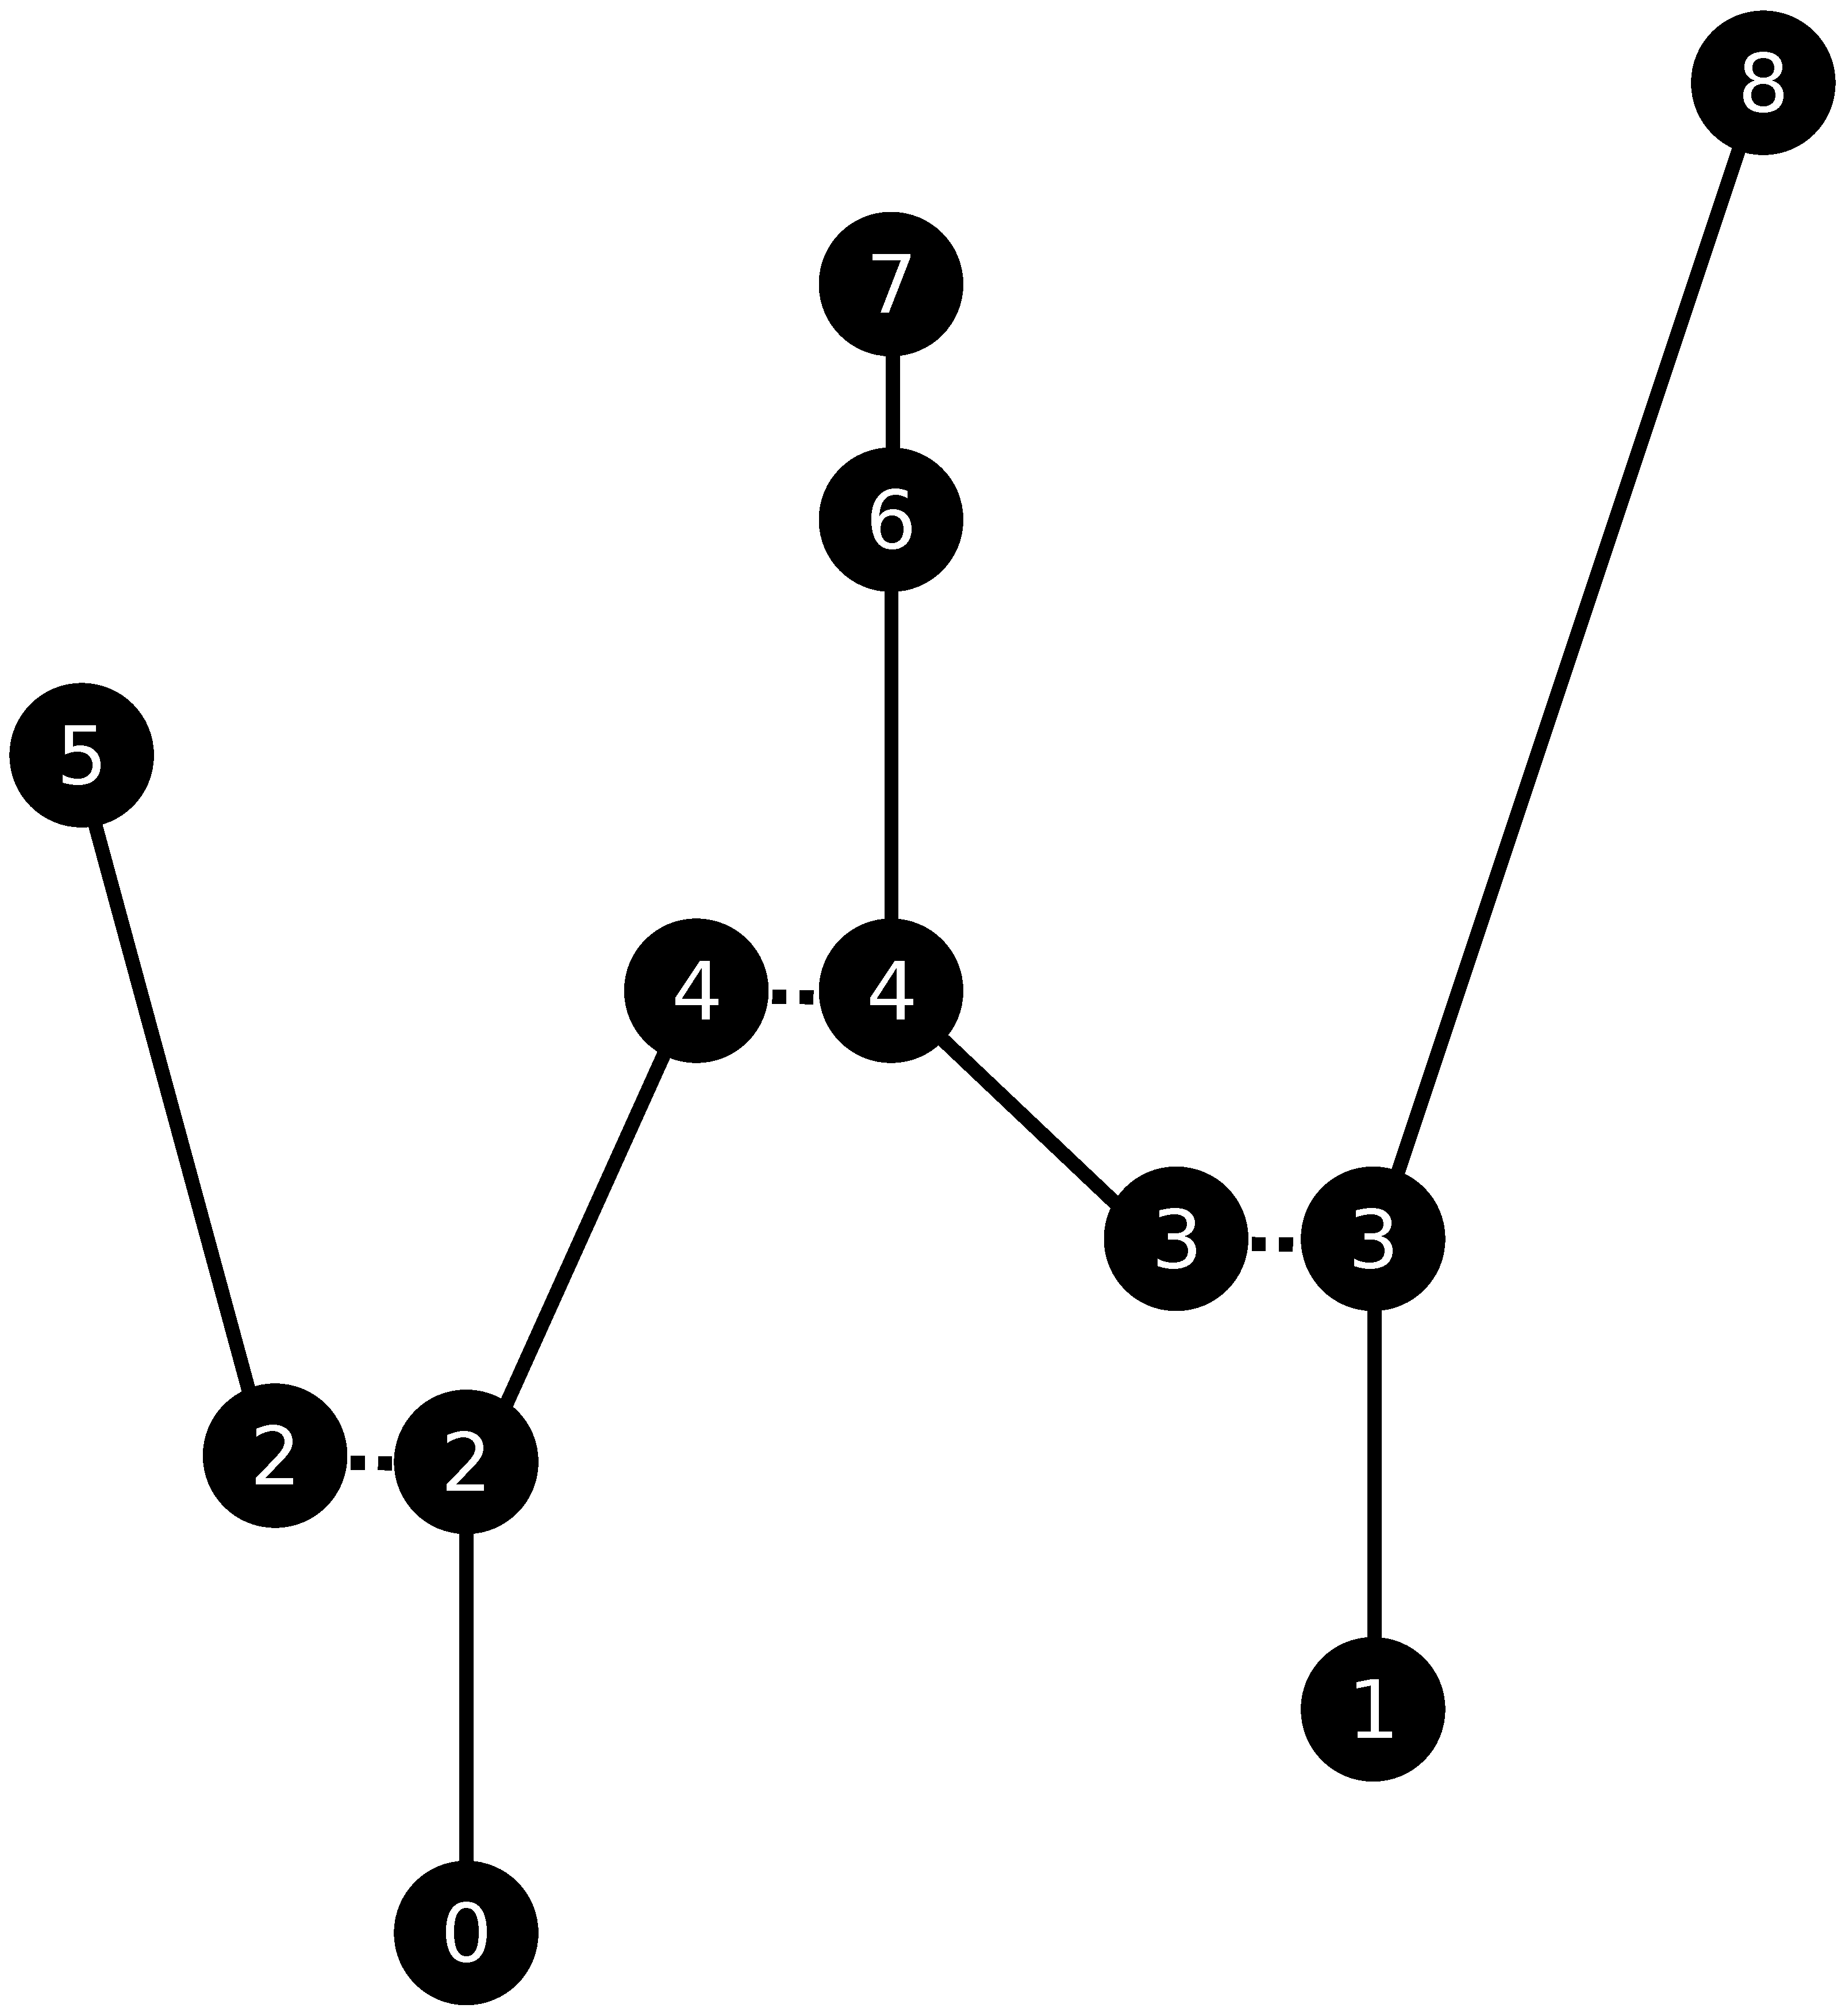
\includegraphics[scale=0.10]{./images/w3x3-ct-decomp.eps}}}%
    \subfloat[Heirarchical view of the branches.]{{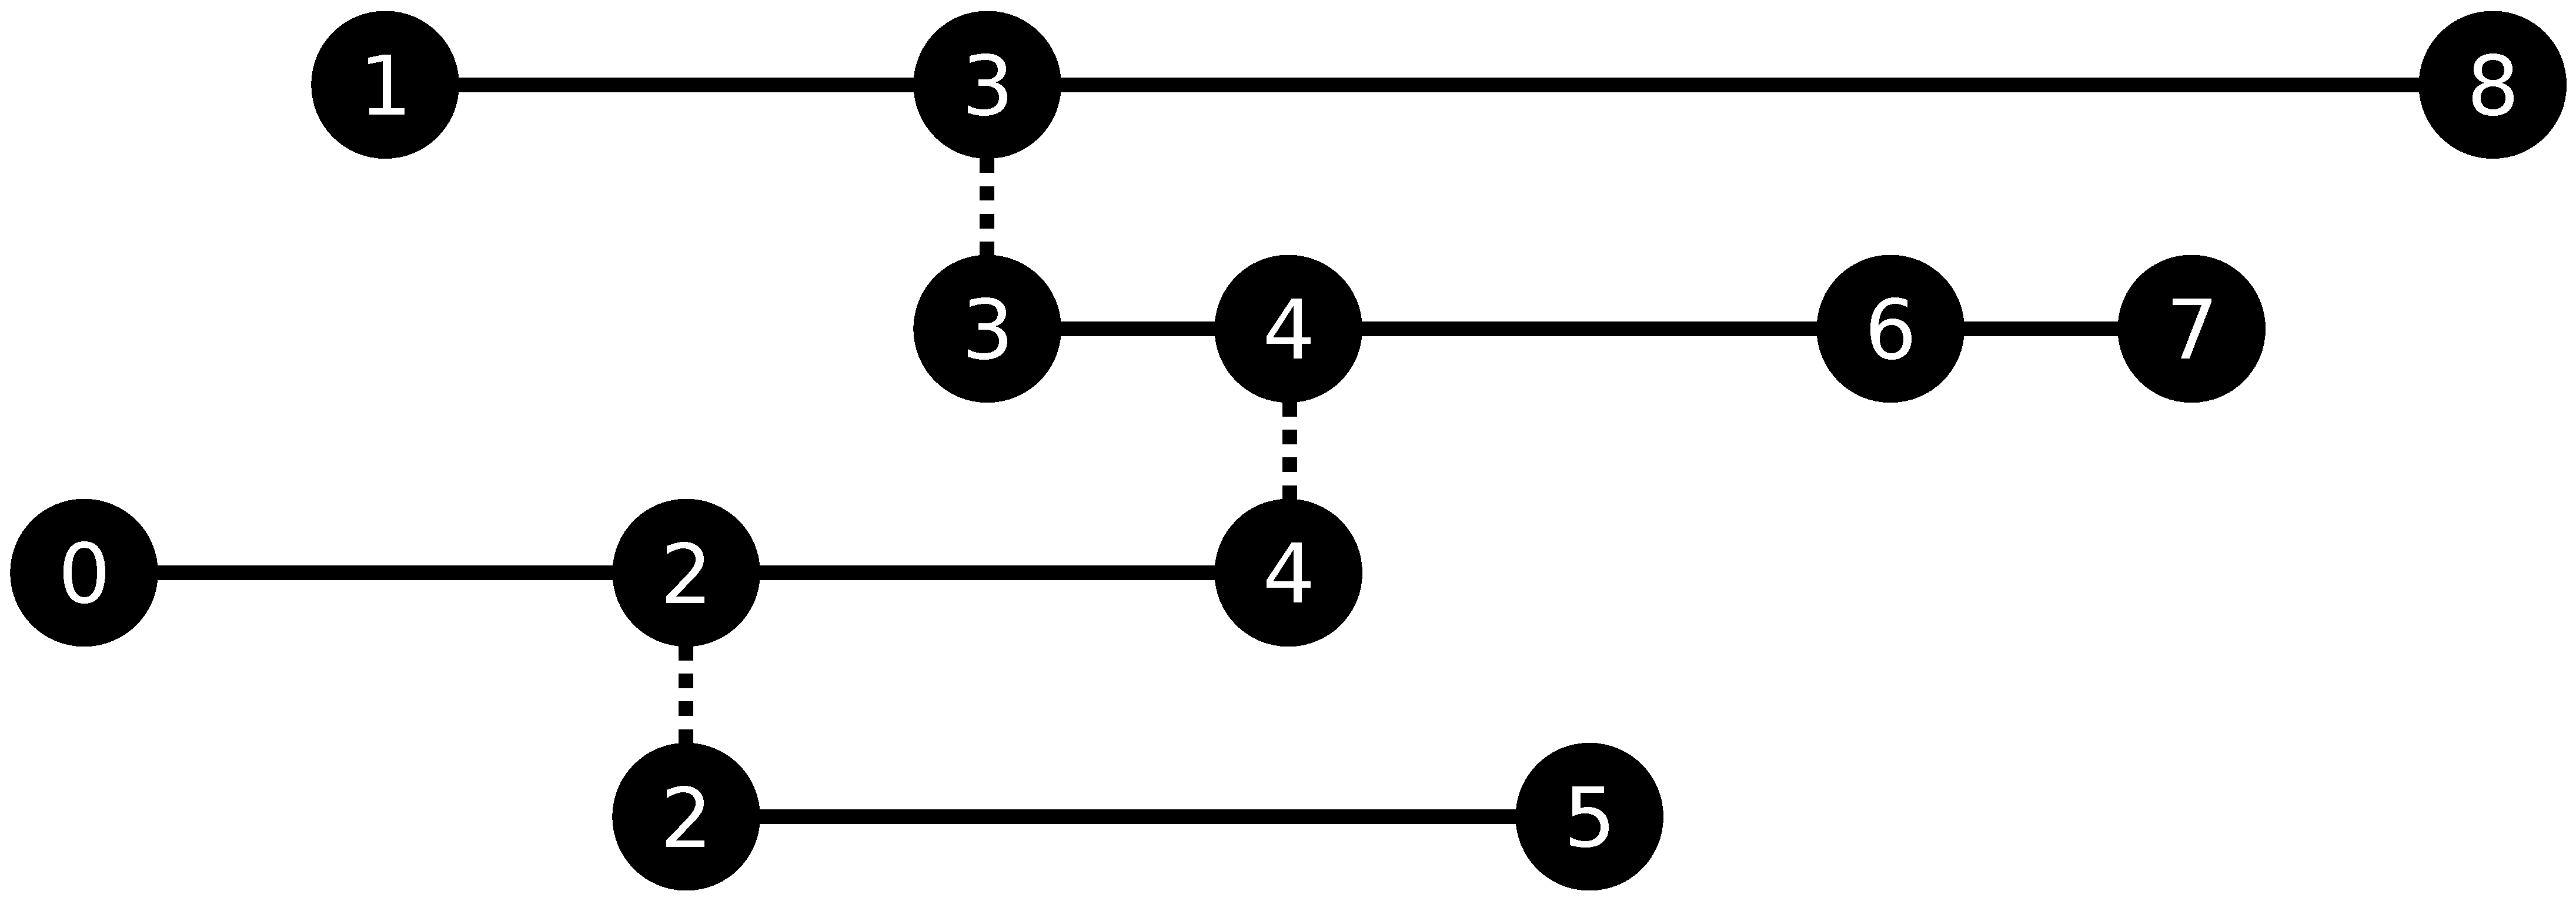
\includegraphics[scale=0.11]{./images/w3x3-ct-h-decomp.eps}}}%
    \caption{Hierarchical branch decomposition of the contour tree from Figure \ref{fig:mesh-join-split-contour} b.}%
    \label{fig:branch-decomp}%
\end{figure}

In the future we will omit the use of hierarchical and just refer to it as branch decomposition. Branch Decomposition is a form of topological simplification whose use is limited to the contour trees. In Chapter 6 we will present a more general topological simplification framework called persistent homology. Our goal will be to express branch decomposition in the framework of persistent homology and determine whether the two are equivalent.

% @TODO Todo talk about how this is used to remove noise and artifacts in data.

% @TODO Remove Stay Tuned
% The paper \cite{ct-branch-decomp} cites that the persistence defined in that way is similar to persistence first defined in \cite{persistence-original}. In Chapter N of this dissertation we will demonstrate that this claim is either incorrect of misleading. Stay tuned folks.

\chapter{Persistent Homology and Contour Trees}
\label{chapter4}

In this chapter we shall take a look at one of the tools that has made Computational Topology so viable for topological data analysis in the recent years. This is of course persistent homology. We will develop further develop the mathematical framework of Homology to accomodate this new concept. After this we will take a look at the practical aspect of the computation of Persistent Homology (PH) and its relation to the computation of the Contour Tree.

\section{Induced Maps on Homology}

Before demonstrating the power of Persistent Homology we will take a slight theoretical detour the inroduce the last piece that we are missing that enales its construction. There is a general result in singular homology that shows the interaction of continus maps and homomorphisms between homology groups.

\begin{defn} Let $X$ and $Y$ be two topologicla spaces. Let $f: X \to Y$ be a continuous function. Then $f$ induces a homomorphism $f_*: H_n(X) \to H_n(Y)$ for all $n \in \{0, 1, 2, ...\}$. \end{defn}

This means that if we have a continus function between two spaces we can immediately associate the homology classes of $X$ to those of $Y$. All we have to do to obtain the induced map is to compose with the continous function $f$. The details of this procees are outlines in \cite{algebraic-topology}.


% @TODO WHY?!
This general result is not appropriate for simplicial complexes. WHY?! We need a more tracktable definition to aid us in our computation. We will thus present the following combinatorially flavoured definition given by \cite{combinatorial-algebraic-topology}. 


\begin{defn} Let $X$ and $Y$ be two finite abstract simplicial complexes. A function $f: X \to Y$ is a simplical map when if $\sigma$ is a simplex of $X$ then $f(\sigma)$ is a simplex of $Y$. \end{defn}

The two most important observations we can make based on this defitions are the following:

\begin{itemize}
    \item The composition of two simplicial maps is simplicial.
    \item When $Y$ is a subcompex of $X$ the inclusion map is a simplicial map.
\end{itemize}


% @TODO Define a homology class
The reason why we introduced simplicial maps is so that we can pose the following question. If there is a simplical map between two simplicial complexes, can we use it to relate their homology classes? The answear is yes, we can thanks to \cite{combinatorial-algebraic-topology}!


% @TODO Are simplicial maps continuous?

\begin{defn} Let $X$ and $Y$ be two simplical complexes and $f: X \to Y$ be a simplicial map. Then $f$ induces a homomorphism $f_*: H_n(X) \to H_n(Y)$ for all $n \in \{0, 1, 2, ...\}$. \end{defn}

The homomorphism is induces by taking the simplicies of a chain through the simplicial map and the considering the homology class the chain ends up in (if any). Detail on this can be found in \cite{combinatorial-algebraic-topology}.

We will further expand this definition to also cover relative chain maps and relative homologies.

\begin{defn} Let $X$ and $Y$ be two simplical complexes and let $A \subseteq X$ and $B \subseteq Y$ be two subcomplexes. Let $f: X \to Y$ be a simplicial map such that $f(A) \subseteq B$. Then $f$ induces a homomorphism $f_*: H_n(X, A) \to H_n(Y, B)$ for all $n \in \{0, 1, 2, ...\}$. \end{defn}

We will use the shorthand $f: (X, A) \to (Y, B)$ for functions that satisfy the criteria of this definition. The function $f$ is called this a simplicial map between simplicial pairs (analogous to continous map between topological pairs in \cite{algebraic-topology}). 


% @TODO Define absolute homology
The homomorphism is induced by running the relative homology classes through the simplicial map and recording which class their image lands in. The primary type of map we will use in this chapter is a specific kind of simplicial map - the inclusion map. The reason for this will become clear in the following section. In the case of absolute homology when $X$ is a simplicial complex and $A$ is a subcomplex of $X$ there is a natural inclusion map $i: A \to X$ which is injective but not necessarily surjective. It takes the simplicies of $A$ to exactly the same simplicies of $X$ and leaves the simplicies outside of $A$ untouched. 

We shall define the inclusion of relative homology analogously. Let $B$ be another subcomplex of $X$ such that $A$ is also a subcomplex of $B$, or $A \subseteq B \subseteq X$. Then let $i : X \to X$ be the identity map. As $A \subseteq B$ then the restriction $i_A: A \to B$ is a well defined function and therefore $i(A) \subseteq B$. Therefore there is a map $i$ between the pairs $(X, A)$ and $(X, B)$ such that $i(A) \subseteq B$ by the previous definition this map induces a homomorphism $i_* : H_n(X, A) \to H_n(X, B)$.


% @TODO Should I talk about chain maps?
% @TODO Add proof for all of this?

\section{Persistent Homology}

% @TODO Define filtrations.
% @TODO Introduce filtrations and VR complexes.

Persistent Homology emerged in the early 2000s in the this work of \cite{persistence-original}. The original motivation for introducing it was to better model point cloud data through filtrations of Vietoris Ribs complexes. Persistent Homology has since grown into a general methodology that can be applied any filtration of a topological space. To best illustrate what persistent homology is let us consider a filtration of a simplical complex $X$. Example in fig[].

$$ X_0 \subseteq X_1 \subseteq ... \subseteq X_{n-1} \subseteq X_n = X$$

We have obtained a one parameter sequence of nester subcomplexes. Another way to think of this is that we start with simplicial complex and iteratively add new simplicies to it. It is customary to call the index of this filtration time to make it more indicative of a process that evolves in time. We can already compute the homology groups of the individual $X_i$. The key insight in persistent homology was to as the question whether we can track the evolution of individual homology classes in the homology groups as we go from one complex to the next. This is made possible by the subset relation between all of the $X_i$. As discussed in the previous section the inclusion map is the natural map between a set and it's superset. More formally we have inclusion maps $i_{i, j}: X_i \to X_j$ for $i \le j$ because $X_i \subseteq X_{i+1} \subseteq ... \subseteq X_j$. 
By only considering the inclusion maps between consecutive $X_i$ and $X_{i+1}$ we can build the following chain of simplicial complexes


$$ X_0 \overset{i}{\longrightarrow} X_1 \overset{i}{\longrightarrow} ... \overset{i}{\longrightarrow} X_{n-1} \overset{i}{\longrightarrow} X_n$$


% @TODO Introduce Chain Maps
where we have renamed all inclusion maps to $i$ and infer them from context. We have already shown that the inclusion maps are simplical and that simplical maps induce homomorphisms on homology groups through chain maps inducing. This lets us transform the sequence directly to the homology groups like so:

$$ H_n(X_0) \overset{i_*}{\longrightarrow} H_n(X_1) \overset{i_*}{\longrightarrow} ... \overset{i_*}{\longrightarrow} H_n(X_{n-1}) \overset{i_*}{\longrightarrow} H_n(X_n).$$

Here it is important to note that the induced maps $i_*$ do not have to be the inclusion maps on the homology groups. They can easily fail to be injective when for example two homology classes in some $H_n(X_i)$ map to the same homology class $H_n(X_{i+1})$ due to the introduction of a new boundary. This contradicts the fact that inclusion maps are injective. The induces homomorphisms encode the local topological changes in the homology of consecutive complexes in the filtration. We will introduce the following terminology to help us interpret this information:


% @TODO You may not be right about death here
\begin{itemize}
    \item A homology class is \textbf{born} if it is not the image of a class in the previous complex in the filtration under $i_*$.
    \item A homology class \textbf{dies} if its image under $i_*$ is the zero element or when it is merged with another class (they have the same iamge).
    \item A homology class \textbf{persists} if its image under $i_*$ is not zero.
\end{itemize}

In order to produce a detailed computation of the persistent homology of a filtration we would have to compute all homology groups of all complexes and then compute all inclusion maps. Doing so by hand is cumbersome and more importantly far too lengthy. We will avoid doing it in favour of presented diagrams of the evolution of the homology classes and appeal to the reader's geometric and topological intuition to argue their correctness.

*Let us look at the following example. Show a pretty picture and explain it*

Given the persistence homology of a filtration we can pose the question of how we can rank the classes based on their "significance". We are most interested in the classes that persist for a large number of steps in the filtration. Such classes are exactly the ones we consider significant and are said to have high persistence. Ephemeral classes on the other hand are consider to have very low significance and can be neglected. In practise such classes often correspond to statistical noise or sampling error.


% @TODO Should you add X_i here istead of just t_i?

To quantify this precisely we will produce the so called persistence pairs. A persistence pair $(t_1, t_2)$ is a pairing of two timestamps - the birth and death time of a homology class. Every class is associated with a pair such as this where $t_1$ is the birth time, $t_2$ is the death time and the class has persisted in all $t_1 \le t_i \le t_2$. In the cases of classes that never die such as *this one in that example* we will assume that their death time is $\infty$. We will call such classes essential and others inessential as in \cite{comp-topo}.

% @TODO Why is this true?
There is a theorem that states that the persistence digram of a filtration encodes all of the information about the persistent homology groups.

*Examples*

Finally we will describe an algorithm for computing the persistence pairs. It requires us order all of the simplices in the complex $\sigma_1, \sigma_2, ..., \sigma_n$ according to these rules \cite{ph-a-survey}.

\begin{itemize}
    \item $\sigma_i$ precedes $\sigma_j$ when $\sigma_j$ was introduced later in the filtration than $\sigma_i$
    \item $\sigma_i$ precedes $\sigma_j$ when $\sigma_i$ is a face of $\sigma_j$
\end{itemize}

Not instead of having to compute the homology groups of all complexes in the filtration individually and then computing the induces maps we can perform the whole computation in a single matrix reduction. Let $D$ be an $n\times n$ matrix and such that.

   $$
   D[i, j] = \left\{
       \begin{array}{@{}l@{\thinspace}l}
           \text{1}  &: \text{if } \sigma_i \text{ is a codimension 1 face of } \sigma_j \\
           \text{0}  &: \text{otherwise} \\
       \end{array}
   \right.
   $$

In other matrix $D$ is a matrix that holds the boundaries of all simplicies in a single matrix. It is called the combined boundary matrix. Now we can perform the following reduction just by column operations.


\begin{algorithm}
\caption{Reduce Combined Boundary Matrix}

\begin{algorithmic}[1]


\ForAll {j $\in$ \{1, 2, ..., n\}} 
    \While {$\exists j': j' < j \text{ and } low(j') == low(j) $}
        \State Add column $j'$ to column $j$.
    \EndWhile
\EndFor

\end{algorithmic}
\end{algorithm}

The proof of this algorithm is outlined in \cite{persistence-original}.

% @TODO What kind does the manifold have to be?
Now let us apply this general theory to a Morse theoretic context. Let $M$ be a triangulation of a smoothly embeded 2-manifold in $\mathbb{R}^3$ and let $f : M \to \mathbb{R}$ be a Morse function. From Morse theory we know that the changes in topology can only happen at finitely many critical points of $M$. Let $c_1 < c_2 < ... < c_n$ be those critical points. Let us now use the sublevel sets $M_{c_i}$  to make a filtration of $M$.We obtain the following filtration which we will call ascending

$$ M_{c_1} \subseteq M_{c_2} \subseteq ... \subseteq M_{c_{n-1}} \subseteq M_{c_n} = M.$$

From this filtration we can produce the following persistent homology chain

$$ H_n(M_{c_1}) \overset{i_*}{\longrightarrow} H_n(M_{c_2}) \overset{i_*}{\longrightarrow} ... \overset{i_*}{\longrightarrow} H_n(M_{c_{n-1}}) \overset{i_*}{\longrightarrow} H_n(M_{c_n}) = H_n(M).$$

If we had taken the superlevel sets of $M$ we would have obtained a different filtration. We will call that the descending filtration of $M$.

$$ H_n(M^{c_1}) \overset{i_*}{\longrightarrow} H_n(M^{c_2}) \overset{i_*}{\longrightarrow} ... \overset{i_*}{\longrightarrow} H_n(M^{c_{n-1}}) \overset{i_*}{\longrightarrow} H_n(M^{c_n}) = H_n(M).$$


Let us now restrict $M$ to be compact and contractable. This will ensure that the Reeb Graph of $M$ is a Contour Tree. We would like to tackle the claim made in \cite{ct-branch-decomp} that the persistent homology pairs are equivalent to branch decomposition pairs. We can immediately see that this claim is either false of ill-defined. The major reason for this is that essential homology classes do not get paired. But in the branch decomposition schemes all critical points are paired.

There is however yet more reason to pursue this. Slightly after the paper of branch decomposition was published, there emerged a way to extend the persistent homology scheme so that all critical points get paired. Using this will allows us to directly compare it to the branch decomposition of a contour tree. 

%We will now show that computing the persistent homology of the descending and ascending filtration of $M$ is equivalent to constructing the join and split tree of $M$ respectively.

%* Show that this is the case *

%* SHOW EXAMPLES *

%Define extended persistence.

\section{Extended Persistence}

We have seen from the definition and computations of persistent homology that not all critical points are paired. Those that give birth the essential persistent homology classes will not be paired because they are never destoyed pass the final simplex in the filtration. This leads to incompleteness in the persistence pairings which we would to remedy. 

* Give example with a previous example where the global minimum was not paired *

**REDO THIS**

We would also like to pair them in such a way that is both symmetric and consistent with our intuition (developed in the example above). Enter extended persistence. The main idea behind extended persistence is to follow the ascending pass of persistent homology with a descending pass where once we reach a class that is homologous to a essential class in the ascending filtration we consider it to be destroyed and thus paired. To justify this algebraically we would like this process to be a consequence of a new augmented chain that starts with the zero homology group and ends with the zero group. This way we have an assurance that every class that is born will eventually die.

Our initial instinct here might be to just directly apply persistent homology twice. Once on the ascending and the on the descending filtration. The problem that arises is in relating the classes of the two different filtrations. It would be ideal if we could merge both filtrations into a single long chain, but the two filtrations flow in different directions. Here is an example

$$ 0 = H_n(M_{c_1}) \rightarrow ... \rightarrow H_n(M_{c_n}) = H_n(M) = H_n(M^{c_1}) \leftarrow ... \leftarrow H_n(M^{c_{n}}) = 0.$$

Here the direction of the arrows is according to the inclusion maps as we have that $M_{c_i} \subseteq M_{c_j}$ and $M^{c_j} \supseteq M^{c_j}$ for $i \le j$. The can be remedied if we reverse the directions of the arrows in the descending filtration. In order to reverse the directions of the arrows and to keep some of our intuition we shall employ the use of relative homology. The following is not equivalent to the previous but is exactly what we are looking for.

$$ 0 = H_n(M_{c_1}) \rightarrow ... \rightarrow H_n(M_{c_n}) = H_n(M) = H_n(M, M^{c_n}) \rightarrow ... \rightarrow H_n(M, M^{c_{1}}) = 0.$$

Where the descending filtration is represented through the sequence of relative homology groups. Let us explore why this is built this way.

The maps in the ascending filtrations are induced via the inclusion maps between the nested spaces $M_i \subseteq M_j$  where $i \le j$. The more interesting case if between the relative homology groups. First of all the isomorphism between $H_n(M) = H_n(M, M^{c_n})$ comes from that fact that $M^{c_n} = \emptyset$ and quotienting by the empty sets leaves a group unchanged. The show where the consecutive maps come from we will give the following example.

Let $X$ be a simplical complex, $B \subset X$ be a subcomplex of $X$ and $A \subset B$ be a subcomplex of $B$. Then we can find a natural map from $H_n(X, A)$ to $H_n(X, B)$ induced by the inclusion from $A$ to $B$. Let us write out $C_n(X), C_n(A), C_n(B)$ through their generator simplicies.

% @TODO Fix these brackets
$$ C_n(X) = <a_1, a_2, ..., a_k, ..., a_l, ..., a_n> $$
$$ C_n(A) = <a_l, ..., a_n>$$
$$ C_n(B) = <a_k, ..., a_l, ..., a_n>$$


Then the relative chains are generated by:

$$ C_n(X, A) = <a_1, ..., a_k, ..., a_{l-1}>$$
$$ C_n(X, B) = <a_1, ..., a_{k-1}>$$


% @TODO Show it is a chain map

Where we can introduce a natural inclusion map $f : C_n(X, A) \to C_n(X, B)$ where $f(a_i) = a_i$ when $i < k$ and $f(a_i) = 0$ when $i \ge k$. The map $f$ is well defined as an inclusion map and furthermore it is a chain map. Chain maps induce linear maps on the homology. Therefore we obtain the map $f_* : H_n(X, A) \to H_n(X, B)$ where $f_*([\alpha]) = [f(\alpha)]$. Where the brackets denote the homology quotient classes in $H_n(X, A) \text{ and } H_n(X, B)$ respectively.

%Now let us to back to the descending filtration of $M$. We have 

Let us go back extended persistence. In the descending filtration of the relative homology we have the scenario we just described. Therefore as there is an inclusion function for between every $M^{c_i}$ and every $M^{c_j}$ where $i \ge j$ and this induces a linear map between every $H_n(M, M^{c_i})$ and $H_n(M, M^{c_j})$.

%We have developed all this mathematical machinery

-- Give some intuition behind this.

-- Show how this is used on an example.

-- Give an algorithm for computing it.

-- Explain how the algorithm is connected to the computation.

\section{Persistent Homology and the Contour Tree}

-- Say some general things about how we are going to relate the two and what we shall accomplish in this chapter.

\subsection{Join and Split Trees}

Show that the computation of the ascending filtration and descending filtration is equivalent to the join and split tree of a contractable domain.

Show the it is equivalent to branch decomposition of the join and split tree.

Show that extended persistence pairing are not equivalent to branch decomposition pairing. Say the paper is either wrong or had something else in mind which is not clarified well enough.

Emerge victorious and have the plebeians chant you name in the streets. All Hail Petros all hail Petros.


\subsection{Extended Persistence on Path-Connected Domains}

The final step we take on this journey will be to prove a more an original and more general results that will solidify our claim completely.


\begin{prop} In the extended persistence of a Path-Connected domain the global minimum pairs with the global maximum in the 0th homology \end{prop}

\begin{proof}
    Let $M$ be a Path-Connected domain and let $M_1 \subseteq M_2 \subseteq ... \subseteq M_n$ be a filtration of $M$. This filtration induces etended persistence 

$$ 0 = H_0(M_{c_1}) \rightarrow ... \rightarrow H_0(M_{c_n}) = H_0(M) = H_0(M, M^{c_0}) \rightarrow ... \rightarrow H_0(M, M^{c_{1}}) = 0.$$

As $M$ is Path-Connected it has one path-connected component and therefore $H_0(M) = H_0(M_0) \simeq  \mathbb{Z}_2$.  Our aim here will be to show that all of the $H_0(M, M^{c_i})$ are trivial. This will mean that the single homology class that exists in $H_0(M)$ will die at $H_0(M, M^{c_n})$ which is exactly the global maximum.


% @TODO Define Excision
% @TODO  Add the thing where this holds - H_n(M / M^{c_i}, pt) = \overset{\sim}{H}_n(M / M^{c_i})
As a corollary of the Excision Theorem we have that

$$H_0(M, M^{c_i}) = H_0(M / M^{c_i}, pt) = \overset{\sim}{H}_0(M / M^{c_i})$$  

where $pt = M^{c_i} / M^{c_i}$.

Now let us explore the reduced homology of the topological space $M / M^{c_i}$. We will show that is it path-connected and therefore the reduced homology is trivial.


% @TODO Add quote
By definition $M$ is path connected. Consider the function $\pi: M \to M/ M^{c_i}$ that takes a point to it's equivalent class. By point set topology [] we know that $\pi$ is continuous. We can also infer that $\pi$ is surjective. Indeed there there is no equivalence class that no point maps to. Furthermore the continuous image of a path connected is connected by []. As we have that $M$ is path-connected therefore $\pi(M) = M / M^{c_i}$ is path-connected. 

By [] we have that $H_0(M / M^{c_i}) = \mathbb{Z}_2$ and by [] that $H_0(M / M^{c_i}) = \overset{\sim}{H}_0(M / M^{c_i}) \bigoplus \mathbb{Z}_2$

We can conclude that $H_0(M, M^{c_i}) = \overset{\sim}{H}_0(M / M^{c_i}) = 0$

Therefore the map induced by the inclusion of the pairs $(M, \emptyset) \to (M, M^{c_n})$ will map the essential homology class of $H_0(M_n)$ to zero. This mean that the global minimum pairs with the global maximum.


\end{proof}










\chapter{Homology}
\label{chapter5}

In this chapter we will shift our attention back to algebraic topology and more specifically the field of Homology. We will use Homology to analyse the connectivity, number of the holes and voids in a simplical complex. We are putting all this work in Homology because it is a prerequisite to one of the leading tools in topological data analysis - Persistent Homology. In the next chapter we will analyse some of the similarities between persistent homology computations and contour tree computations.

\section{Homology}


% @TODO Fix introduction

The guiding principle behind the Euler Characteristic was to decompose a space into cells, count them and perform cancellations based on the parity of the dimension of the cells. This approach yields valuable information about a topological space, but we can hope to gain more by generalising it. We shall accomplish this by leveraging the mathematical machinery of Homology. Homology is a tool that was first developed to measure the topological complexity of manifolds \cite{persistence-original}. For example with homology we can recognize that there is a hole in the torus and a volume enclosed in the sphere. The theory of Homology comes in two flavours - \textbf{simplical} and \textbf{singular}. Simplicial homology is geared towards analysing simplical complexes and singular homology is the appropriate generalisation for arbitrary topological spaces. In this dissertation we restrict attention on singular homology because we are primarily interested in the computational aspect of homology.

%We will however on occasion refer to singular homology when we desire to leverage a more general result from the relevant theory. More information on singular homology can be found in the following sources \cite{algebraic-topology, elementary-applied-topology}


Homology is built around the interplay between two key concepts of \textbf{cycles} and \textbf{boundaries}. Let us consider the simplical complex depicted on Figure \ref{fig:hom-sc} as an example. It consists of four vertices $\{a, b, c, d\}$, five edges $\{ab, bc, ca, db, cb\}$ and one face $\{abc\}$. Let us first explain what a boundary is. The boundary of a simplex consists of its codimension-1 faces. For example the boundary of the 1-dim simplex $ab$ consists of the 0-dim simplices $a \text{ and } b$. The boundary of the 2-dim simplex $abc$ consists of the 1-dim simplices $ab, ac \text{ and } cb$. A cycle on the other hand consists of the simplices that form the boundary of a simplex that is of one dimension higher (regardless of whether that one dimension simplex is in the complex). In our example we can observe that the edges $ab, bc, ca$ and $bd, dc, cb$ form a 1-dim cycle because they are the boundary of the-dimensional simlices $abc$ and $bdc$. The first simplex $abc$ is in the complex while $bdc$ is not. The definition of one dimensional cycles is in line with the graph theoretic definition. The first and last vertex of the paths formed by those edges are the same. A more geometric way to put it is that the edges enclose an 2-dim area of space. To expand this definition to higher dimensional cycles picture the faces of the tetrahedron. They would form a 2-cycle as they completely enclose a 3-dim volume. In general an n-cycle consists of simplices that are the boundary of a n+1-dim simplex

\begin{figure}[h]%
    \centering
    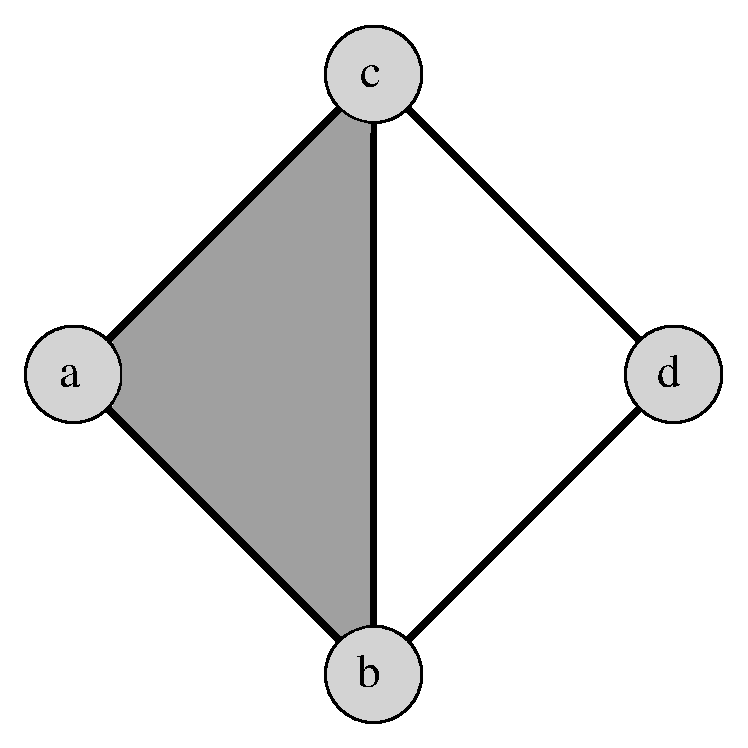
\includegraphics[scale=0.4]{./images/chapter1/homology-sc.eps}%
    \caption{An Example Simplical Complex}%
    \label{fig:hom-sc}%
\end{figure}

The interplay between between cycles and boundaries is in asking the question - which cycles in the complex are \textbf{not} the boundary of a higher dimensional simplex. Such cycles are important because they introduce a void in the space. Cycles which are the boundary of a higher dimensional simplex can be disregarded because the void they introduces is filled by that higher dimensional simplex. Coming back to our example the cycle $ab, bc, ac$ is the boundary of $abc$, but the cycle $db, cd, bc$ it not the boundary of another simplex in the simplical complex. The cycle $db, cd, bc$ represents a 2-dim hole in the simplical complex. Finally note that the cycle $ab, bd, dc, ac$ is in a sense equivalent to the cycle $db, cd, bc$ because both describe the same 2-dim hole in the complex - namerly the missing 2-dim simplex $bdc$.

%This is important because these cycles cannot be contracted to a point. The lack of higher dimensional simplex the enclose means there is a void of some dimension in our simplex.

Notice also that the paths formed by the edges $bc, ca, ab$ and $ac, ab, bc$ represent the same cycle. The only difference is which vertex is the starting and ending point. We would like to disregard the choice of starting point and order of edges completely because for example the paths $bc, ac, ab$ and $ac, ab, bc$  represent the same structure in the simplical complex. Enter additive algebraic notation. In this notation the same cycle would be written as $ab + bc + ca$.

Additive notation implies associativity but it does not have to sole purpose of illustrating the point of disregarding edge order. Its more important aspect is that it allows us to treat sums of edges as linear combinations in an abstract vector space. To begin with, we will operate with vector spaces over the field of coefficients $\mathbb{Z}_2 = \{0, 1\}$ together with the standard operations of addition and multiplication modulo two. We will use abstract vector spaces over the field of coefficients $\mathbb{Z}_2$ as the building blocks of our study of Homology.

Let $X$ be a simplicial complex. An n-chain of $X$ is a formal sum of n-simplices of $X$ \cite{comp-topo}. The notation we will use for an n-chain is $\sum{a_i \sigma_i}$ where $a_i \in \mathbb{Z}_2$ and $\sigma_i$ is an n-simplex of $X$. We can add two n-chains component wise much like we would add polynomials. For example $(ab + bc) + (ab + cd + db) = 2ab + bc + cd + db = bc + cd + bd$ because $2 = 0$ in $\mathbb{Z}_2$.

Based on the n-chains of $X$ we can define the \em chain complex \em of $X$. It is made up of the following vector spaces and linear maps between them:

\begin{itemize}

    \item The \textbf{group of n-chains} $C_n(X)$ of $X$. These are the vector spaces where the vectors are all possible n-chains of $X$ and the coeficients are $\mathbb{Z}_2$.

    \item The \textbf{boundary maps} $\partial_n$ between the groups of n-chains of $X$. These are linear maps between consecutive groups of n-chains $\partial_n : C_n(X) \to C_{n-1}(X)$.

\end{itemize}

What we have defined as the chain complex of $X$ is no more that a collection of vector spaces together with linear maps between. When n is smaller than zero bigger than the dimension of $X$ then the approriate vector space is the trivial, consisting only of the zero element. We can visualise the chain complex of $X$ with the so called quiver representation. For our example simplical complex it would look like:

$$ 0 \overset{\partial_{3}}{\longrightarrow} C_2(X) \overset{\partial_{2}}{\longrightarrow} C_{1}(X) \overset{\partial_{1}}{\longrightarrow} C_{0}(X) \overset{\partial_0}{\longrightarrow}  0 $$

In the general case for an n-dimensional simplical complex $X$ the full chain complex would be:

$$ ... \longrightarrow 0 \overset{\partial_{n+1}}{\longrightarrow} C_n(X) \overset{\partial_{n}}{\longrightarrow} C_{n-1}(X) \overset{\partial_{n-1}}{\longrightarrow} ... \longrightarrow  \overset{\partial_1}{\longrightarrow} C_0(X) \overset{\partial_0}{\longrightarrow} 0 \longrightarrow ... $$

where we can extend both right and lefthand sides with the zero vector spaces and zero maps infinitely. More specifically in this sequence $\partial_{n+1} \text{ and } \partial_{0}$ are zero maps. The boundary map $\partial_{n+1}$ sends the zero vector of $0$ to the zero vector of $C_n(X)$ and the map $\partial_0$ sends all vectors in $C_0(X)$ to the zero vector in $0$.

Let us now expand on how the groups of n-chains and the boundary maps of a simplical complex are constructed explicitly. In our working example $C_0(X)$ is the vector space that is spanned by the vertices $\{a, b, c, d\}$ of the complex. We write this as $C_0(X) = span(\{a, b, c, d\})$. A vector in $C_0(X)$ is a linear combination of the basis vectors using coefficients in $\mathbb{Z}_2$. Let $\sigma \in C_0(X)$ be a vector, then we can express it as $\sigma  = \alpha_0a + \alpha_1b + \alpha_2c + \alpha_3d$ where $\alpha_i \in \{0 ,1\}$ for every $i = 0, 1, 2, 3$. Going a dimension up $C_1(X) = span(\{ab, bc, ca, cd, bd\})$. As we pointed out earlier the cycle that consists of the edges $bc, cd, db$ is represented by the sum or linear combination $bc + dc + bd = 0ab + 1bc + 0ca + 1cd + 1bd$ and has coordinates $(0, 1, 0, 1, 1)$ in $C_1(X)$ with respect to the basis we have chosen. We may of course work in any basis we like. For example $C_0(X) = span(\{a + b, b, c, c + d\})$ because the vectors $(1, 1, 0, 0), (0, 1, 0, 0), (0, 0, 1, 0) \text { and } (0, 0, 1, 1,)$ are linearly independent. In this basis the 0-simplex $a + b + c + d$ will have coordinates $(1, 0, 0 1)$.

The boundary maps are defined analogously to how we presented them in the beginning of the section. The effect a boundary map has on a simplex $\sigma \in C_n(X)$ is that it returns the linear combination consisting of the simplices of $C_{n-1}(X)$ that are codimension-1 faces of $\sigma$. If $\sigma$ is the convex  combination of the vertices $[v_0, v_1, ..., v_n]$ then we define it's boundary as

$$ \partial(\sigma) = \partial([v_0, v_1, ..., v_n]) = \sum_{i=0}^{n}[v_0, ... , \hat{v_i}, ..., v_n] ,$$

where the hat on top of $v_i$ signifies that we omit it in the convex combination. From this definition we can extend $\partial$ linearly by allowing it commute with vector addition and scalar multiplication like so:

$$ \partial\bigg(\sum_{\sigma}a_{\sigma}\sigma\bigg) = \partial\bigg(\sum_{\sigma}{a_{\sigma}[v_{\sigma_0}, v_{\sigma_1}, ..., v_{\sigma_n}]}\bigg) = \sum_{\sigma}{a_{\sigma} \sum_{i=0}^{n}[v_{\sigma_0},..., \hat{v}_{\sigma_i}, ..., v_{\sigma_n}]} .$$

Going back to our working example let $\sigma = ab + bc + ca$ be an n-chain in $C_{1}(X)$. Then $\partial(ab + bc + ca) = \partial(ab) + \partial(bc) + \partial(ca) = a + b + b + c + c + a = 2a + 2b + 2c = 0$. This examples allows us to observe an important fact. We know that the n-chain $ab + bc + ca$ is a cycle and we obtained that it's boundary is zero. This is no concidence. The defining feature of a cycles is that they have no boundary. In general the n-cycles in $C_{n}(X)$ are exactly the n-chains that go to zero under the boundary map. The set of all vector that go to zero under a linear map is known as the kernel of the linear map. The kernel of the boundary map $\partial_n : C_{n}(X) \to C_{n-1}(X)$ is denoted as:

$$ Z_n = ker(\partial_n) = \Big\{\sigma \in C_{n}(X): \partial_n\big(\sigma\big) = 0 \Big\}. $$

We can also translate the boundaries in the language of linear algebra. The boundaries in $C_n(X)$ are given by the image of $C_{n+1}(X)$ under $\partial_{n+1}$. We write this as:


$$ B_n = im(\partial_{n+1}) = \Big\{\partial_{n+1}(\sigma) \in C_{n}(X): \sigma \in C_{n+1}(X) \Big\}. $$


%Let us now translate the geometric intuition we have of cycles and boundaries to domain of linear algebra. The boundaries are provided to us by the boundary maps. Thus the set of all boundaries in $C_n(X)$ is given by the image of $C_{n+1}(X)$ under $\partial_{n+1}$ or $im(\partial_{n+1})$. The cycles in $C_n(X)$ are given by all the vectors in $C_n(X)$ that go to the zero vector of $C_{n-1}(X)$ under $\partial_n$. Intuitively the boundary of an n-chain is zero exactly when all of the faces of the simplices in the chain have even parity and cancel in our binary algebra. The set of all vectors that go to the zero vector under the boundary map $\partial$ is precisely the kernel of $\partial$ or $ker(\partial)$.

%From linear algebra we know that for a linear function $f: V \to W$, $ker(f)$ is a linear subspace of $V$ and $im(f)$ is a subspace of $W$. In the context of chain complexes this means that the images and kernels of all the boudary maps are linear subspaces of their respective n-chains. Before learning how the interplay between cycles and boundaries is translated in this setting we must present the following fundamental theorem

Now that we have the means of describing the cycles and boundaries the only thing that we are missing is to partition the cycles into groups of cycles that differ from each other only by their boundary. We want of way of making precise the notion that the cycles $ab, bd, dc, ac$ and $db, cd, bc$ in Example [] are equivalent because they both represent the missing simplex $dbc$. To do so we must first understand how $Z_n$ and $B_n$ are related through the fundamental Lemma of Homology.

\begin{lem} Fundamental Lemma of Homology. $(\partial_{n-1} \circ \partial_n) (\sigma) = 0, \text{ for every } \sigma \in C_{n}(X)$. \end{lem}

\begin{proof}
    We will only sketch the intuitive outline of the proof and refer the reader to \cite{algebraic-topology} for a more complete version.

    Let us consider the boundary of $\sigma \in C_n(X)$ which is $\partial_n(\sigma)$. It contains all of the n-1 faces of $\sigma$. Furthermore every n-2 face of $\sigma$ belongs to exactly two n-1 faces of sigma. Therefore they will cancel out in the second boundary operation $\partial_{n-1}\partial_n(\sigma)$.
\end{proof}


\begin{cor}  For every two consecutive boundary maps $\partial_n$ and $\partial_{n-1}$ in a chain complex $im(\partial_n) \subseteq ker(\partial_{n-1})$. \end{cor}

\begin{proof}
    If the image of $\partial_n$ were not in the kernel of $\partial_{n-1}$ then there would be at least one n-chain $\sigma$ for which $(\partial_{n-1} \circ \partial_n) (\sigma) \ne 0$. By the Fundamental Lemma of Homology this is not possible.
\end{proof}

We have found that $B_n \subseteq Z_n$, but we can make an even stronger statement. From linear algebra \cite{lin-alg-done-right} we know that the kernel and image of a linear function are linear subspaces of the domain and range of the linear map. Therefore $B_n$ and $Z_n$ are linear subspaces of $C_n(X)$. As $B_n \subseteq Z_n$ we can infer that $B_n$ is a linear subspace of $Z_n$. In order to partition all cycles in $Z_n$ into equivalence classes of cycles which only differ by a bounday in $B_n$ we can take the quotient of the two spaces. This quotient is in the heart of Homology!

\begin{defn} The n-th homology group of a chain map is the quotient $H_n(X) = Z_p \big/ B_p = ker(\partial_{n+1})\big/im(\partial_n)$. \end{defn}

We know two important things about the quotient $H_n(X)$. The first one is that the quotient of a vector space and its subspace is a vector space \cite{lin-alg-done-right}. The second one is that the dimension of the quotient space is equal to the difference of the dimension of the vector space and the dimension of the subspace \cite{lin-alg-done-right}. Therefore $H_n(X)$ is a vector space and $dim(H_n(X)) = dim(ker(\partial_{n+1})) - dim(im(\partial_n))$. The elements of $H_n(X)$ are called homology classes. For a cycle $\sigma \in Z_p$ we done it's homology class in the quotient $H_p(X)$ as $[\sigma]$. Two cycles are in the same homology class exactly when they only differ by a boundary. In our working example this means that $[ab + bd + dc + ac] = [db + cd + bc]$. Both cycles are representatives of the same homology class.

The dimensions of the homology groups are a summary of the topological information about the connectivity of the n-dimensional simplicies of a complex. They are called Betti numbers and they have the following interpretation.

\begin{itemize}
    \item Betti zero or $\beta_0 = dim(H_0)$ is the number of connected components
    \item Betti one  or $\beta_1 = dim(H_1)$ is the number one dimentional holes in a space or holes.
    \item Betti two  or $\beta_2 = dim(H_2)$ is the number two dimentional holes in a space or voids.
\end{itemize}


The higher Betti numbers represent the number of higher dimensional voids. In a simplicial complex of finite dimension the Betting numbers from a point onwards to all be zero. This of course means that the according homology group are the zero dimensional vector space.

Homology computations are far too envolved and lenghty to be given as examples here. We refer the eager and interested reader to [].

% *Give example with the torus*

% This is exactly what we wanted from Homology. An apparatus that allows us distinguish topological spaces based on the connectivity of their n-dimensional simplical complexes.

% * Leave this or not? *

% Before going forward we must note that we did not have to use coeficients in $\mathbb{Z}_2$ we could have equally used coeficients in $\mathbb{Z}$ but $\mathbb{Z}$ is not a field and we would have obtained that the $C_n(X)$ and $H_n(X)$ are not vector spaces but free abelian groups. If instead we had picked any arbitrary ring we would have obtained free modules instead of free abelian groups. We did indeed lose some information but sticking to vector spaces. The Betti numbers are not always equal, but by the Coeficient Theorem they are for suitably nice spaces. We readily refer the reader to \cite{algebraic-topology} to learn about those. We shall continue the treatment of the subject in the same spirit of vector spaces.

\section{Reduced and Relative Homology}

There are two extensions of homology we need to discuss so that we may to be able to fully harness the power of persistent homology in the following chapter. Those are reduced and relative homology.

The need for reduced homology arises from a slight inconsistency in the interpretation of the homology groups. Take for example the simplical complex that consists of a single vertex. All of its homology groups except for the $H_0$ are trivial. It is convenient in many application to force $H_0$ behave like the rest of the homology group. More specifically, in our example of a single vertex we would like for it's 0th homology group it to be trivial. Consequently we would also like path-connected simplical complexes will have trivial 0th homology. The geometrical interpretation of this extension is the reduced 0th homology classes represent the number of voids that separate path connected components and not the path connected components themselves.

In order to accomplish this we will augment the chain complex of simplical complex $X$ with one additional group $\mathbb{Z}_2$ and one linear map $\epsilon : C_0(X) \to \mathbb{Z}_2$. The resulting chain complex is:

$$ ... \longrightarrow C_1(X) \longrightarrow C_0(X) \overset{\epsilon}{\longrightarrow} \mathbb{Z}_2 \longrightarrow 0 .$$

In this augmented chain the function $\epsilon: C_0(X) \to \mathbb{Z}_2$ is defined as $\epsilon\big(\sum_{i}n_i\sigma_i\big) = \sum_{i}n_i$. The value of $\epsilon$ is equal to the parity of the number of simplicies in the chain. We will define the reduced homology as the homology of the augmented chain complex or $\overset{\sim}{H}_n(X)$. From \cite{algebraic-topology} we have that $\overset{\sim}{H}_n(X) = H_n(X)$ for $n > 0$ and $\overset{\sim}{H}_0(X) \bigoplus \mathbb{Z}_2 = H_0(X)$.

Another crucial concept is that of relative homology. Relative homology aims to simplify the homology of a simplical complex $X$ by discarding all chains that belong to a subcomplex $A$ of $X$. We do so by taking the quotient of the chain groups of $X$ and the chain groups of $A$. We will define this quotients as $C_n(X, A) = C_n(X) / C_n(A)$ and call $C_n(X, A)$ the relative chain groups. As the boundary maps take $C_n(A)$ to $C_{n-1}(A)$ they induce relative boundary maps from $C_n(X, A)$ to $C_{n-1}(X, A)$. The relative bounday map takes a relative class from $[\sigma] \in C_n(X, A)$ to a relative class $[\partial_n(\sigma)] \in C_n(X, A)$. By taking the relative chain groups together with the relative chain maps we obtain the relative chain complex.

$$ ... \longrightarrow C_n(X, A) \longrightarrow ... \longrightarrow C_1(X, A) \longrightarrow C_0(X, A) \longrightarrow 0. $$

We will define the relative homology groups of the relative chain complex as $H_n(X, A) = ker(\partial_n) / im(\partial_{n-1})$ where we substitute $\partial_n$ and $\partial_{n-1}$ to be the relative boundary groups. The most important thing to note is that $H_n(X, A)$ is not the quotient $H_n(X) / H_n(A)$, but the homology of the relative chain complex.

Intuitively here is how we can think of the relative homology classes \cite{algebraic-topology}.

\begin{itemize}
  \item A relative chain $\alpha$ is a relative cycle when it's boundary $\partial_n(\alpha)$ is in $C_n(A)$.
  \item A relative cycle $\alpha$ is trivial in the homology when it's the sum of a boundary $\partial_n(\beta)$ of $\beta \in C_{n+1}(X)$ and a chain $\gamma \in C_n(A)$.
\end{itemize}

There is a connection between the relative chain complex and the reduced chain complex \cite{elementary-applied-topology}. In fact they are equal when we quotient by a single vertex of $X$. Let $p$ be a 0-simplex of $X$ then $\overset{\sim}{H}_n(X) = H_n(X, p)$. The reason for this is that the 0th homology class $p$ becomes trivial in the homology relative to $p$.

The relative homology classes are a purely algebraic construction, but for simplical complexes there is an appropriate geometric intuition that goes along with them. It is expressed through the following theorem \cite{comp-topo}.

\begin{thm} (Excision Theorem)
  Let $K_0 \subseteq K$ and $L_0 \subseteq L$ be two pairs of simplicial complexes that satisfy $L \subseteq K$ and $L - L_0 = K - K_0$. Then they have isomorphic relative homology groups $H_n(K, K_0) \simeq H_n(L, L_0)$.
\end{thm}

% @TODO Should A be a closed subcomplex?
A corollary of the Excision Theorem \cite{elementary-applied-topology} is that if $A$ is a subcomplex of $X$ then $H_n(X, A) \simeq H_n(X/A, A/A) \simeq \overset{\sim}{H}_n(X/A)$ where $A/A$ is a single point in $X/A$. This will allows us to leverage our geometric intuition about quotient spaces to compute homology groups. We will make use of this geometric intuition when we are presenting examples in the next chapter. In particular when $X$ is a small enough simplical complex we will use the Excision Theorem to compute the dimension of $\overset{\sim}{H}_0(X/A)$ by simply counting the number of connected components of $X/A$ and subtracting one.





\section{Inclusion Maps and Induced Maps on Homology}


We will devote this final section to introducing inclusion maps between chain complexes and how they induce linear maps between the homology and relative homology groups of the chain complexes. We will begin by defining inclusion maps:

\begin{defn} Let $X$ be a simplicial complex and $A$ be a subcomplex of $X$. A function $i: A \to X$ is an inclusion map when $i$ takes a simplex $\sigma$ in $A$ to $\sigma$ in $X$.
\end{defn}

In other words $i(\sigma) = \sigma$ and when $A = X$ then the inclusion maps is the identity map. Note that an inclusion maps is a special case of a simplicial map \cite{combinatorial-algebraic-topology}. A simplicial map between two simplical complexes takes simplicies from one to simplicies of the other. An inclusion map fits that cireria by simply mapping all simplicies to themselves. Furthermore inclusion maps will allows us to obtain maps between the chain groups of $A$ and $X$.

\begin{defn} Let $X$ be a simplicial complex and $A$ be a subcomplex of $X$ and $i: A \to X$ be an inclusion map. Then $i$ induces an inclusion map $i_\#: C_n(A) \to C_n(X)$ for all $n \in \mathbb{Z}$. \end{defn}

In order to define $i_\#$ we just have to extend $i$ linearly to n-chains of $C_n(A)$ as follows: $i_\#(\sum a_\sigma \sigma) = \sum a_\sigma i(\sigma)$. Note that $i_\#$ is also an inclusion maps because every n-chain in $C_n(A)$ is also an n-chain of $C_n(X)$ and $i$ maps simplicies to themselves. Upon obtaining inclusion maps between the chain complexes of $A$ and $X$ we can take a step further and induce a linear map between the homology groups of $A$ and $X$.

\begin{defn} Let $X$ be a simplicial complex and $A$ be a subcomplex of $X$ and $i_\#: C_n(A) \to C_n(X)$ be an inclusion map. Then $i_\#$ induces an linear map $i_*: H_n(X) \to H_n(Y)$ such that $i_*([\sigma]) = [i_\#(\sigma)]$ for all $n \in \mathbb{Z}$.
\end{defn}

Where $[\sigma]$ is the homology group of a an n-chain $\sigma$ in $C_n(A)$ and $[i_\#(\sigma)]$ is the homology group of a an n-chain $i_\#(\sigma) = \sigma$ in $C_n(X)$. A crutial thing to note here is that $i_*$ does not have to be an inclusion map between the homology groups. Take for example a cycle which is not trivial in $H_n(A)$. The same cycle could become trivial in $H_n(A)$ if $X$ contain a simplex whos boundary is $\sigma$, but $A$ does not not.

The last thing we will do it to expand the definitions we've made for far to relative homology groups.

\begin{defn} Let $X$ be a simplicial complex. Let $A$ and $B$ be two subcomplexes $X$ such that $A \subseteq B$. Then the identity map $i: X \to X$ induces a linear map $i_*: H_n(X, A) \to H_n(X, B)$ for all $n \in \mathbb{Z}$.
\end{defn}

To see why this holds we refer the reader to \cite{algebraic-topology}. One just has to keep in mind that the identity map is a well defined continous map between topological pairs such as $(X, A)$ and $(X, B)$.

% To see why this is true first observe that $i$ induces an identity map between $C(X)$ and $C(X)$. This idetity map takes $C_n(A)$ to $C_n(B)$ and so we can create a well defined map $i_\#: C(X, A) \to C(X, B)$ such that $i_\#([\sigma]_A) = [\sigma]_B$. This map clearly commuted with the relative boundary map, therefore it induces a linear map on the relative homology groups.

% is an identity map then $i_\#(A) \subseteq$

% To see why this is true observe that the identity map $i: X \to X$ induces a linear map $i_\#: C(X, A) \to C(X, B)$ because the

% This implies that



% The homomorphism is induced by taking the simplicies of a chain through the simplicial map and the considering the homology class the chain ends up in (if any). Detail on this can be found in \cite{combinatorial-algebraic-topology}. We will further expand this definition to also cover relative chain maps and relative homologies.
%
% \begin{defn} Let $X$ and $Y$ be two simplical complexes and let $A \subseteq X$ and $B \subseteq Y$ be two subcomplexes. Let $f: X \to Y$ be a simplicial map such that $f(A) \subseteq B$. Then $f$ induces a homomorphism $f_*: H_n(X, A) \to H_n(Y, B)$ for all $n \in \{0, 1, 2, ...\}$. \end{defn}
%
%
%
% We will further expand this definition to also cover relative chain maps and relative homologies.
%
% \begin{defn} Let $X$ and $Y$ be two simplical complexes and let $A \subseteq X$ and $B \subseteq Y$ be two subcomplexes. Let $f: X \to Y$ be a simplicial map such that $f(A) \subseteq B$. Then $f$ induces a homomorphism $f_*: H_n(X, A) \to H_n(Y, B)$ for all $n \in \{0, 1, 2, ...\}$. \end{defn}
%
% We will use the shorthand $f: (X, A) \to (Y, B)$ for functions that satisfy the criteria of this definition. The function $f$ is called a simplicial map between simplicial pairs (analogous to continuous map between topological pairs in \cite{algebraic-topology}).


% We will devote this final section to introducing simplicial maps between chain complexes and how they induce linear maps between the homology and relative homology groups of the chain complexes. We will begin by defining simplicial maps \cite{combinatorial-algebraic-topology}.
%
% \begin{defn} Let $X$ and $Y$ be two simplicial complexes. A function $f: X \to Y$ is a simplical map if it takes every simplex $\sigma$ of $X$ to a simplex $f(\sigma)$ of $Y$ and furthermore the dimensions of $\sigma$ and $f(\sigma)$ are equal.
% \end{defn}
%
% The definition we use here is more restrictive than that in \cite{combinatorial-algebraic-topology} because it requires that simplicial maps preserve the dimensions of simplicies. We have altered the definition for two reasons. First to simplify the treatment of the subject and second because we will only be making use of inclusion maps between a subcomplex and a complex.
%
% Simplicial maps play an important role in Homology. If we establish a simplicial map between two simplicial complexes we can use it to obtain a map between the chain groups of the simplical complexes. We will such a map a chain map.
%
% \begin{defn} Let $X$ and $Y$ be two simplical complexes and $f: X \to Y$ be a simplicial map. Then $f$ induces a chain map $f_\#: C_n(X) \to C_n(Y)$ for all $n \in \mathbb{Z}$. \end{defn}
%
% The chain map is induced by linearly extending $f$ to chains in the chain groups and applying it to simplicies of $X$. It is defined as $f_\#(\sum_ia_i\sigma_i) = \sum_i a_i f(\sigma_i)$. Upon obtaining chain maps between the chain complexes of $X$ and $Y$ we can a step further a induce a linear map between the homology groups of $X$ and $Y$.
%
% \begin{defn} Let $X$ and $Y$ be two simplical complexes and $f: X \to Y$ be a simplicial map. Then $f$ induces a linear map $f_*: H_n(X) \to H_n(Y)$ such that $f_*([\sigma]) = [f_\#(\sigma)]$ for all $n \in \mathbb{Z}$. \end{defn}
%
% Where $[\sigma]$ is the homology group is a an n-chain in $C_n(X)$ and $[f_\#(\sigma)]$ is an

% We define such that $f_#(\sigma) = f(\sigma)$


% where $\sigma$ is a simplex of $X$ and $f(\sigma)$ is a simplex of $Y$ because $f$ is a simplicial map.

% Simplicial maps play an important role in Homology. If we establish a simplicial map between two simplicial complexes we can use it to obtain a map between the homology groups of the simplicial maps. This new map is called an incuded linear map.

% \begin{defn} Let $X$ and $Y$ be two simplical complexes and $f: X \to Y$ be a simplicial map. Then $f$ induces a linear map $f_*: H_n(X) \to H_n(Y)$ such that $f_*([\sigma]) = [f(\sigma)]$ for all $n \in \mathbb{Z}$. \end{defn}

% In the definition $[\sigma]$ is the homology class of $\sigma$ in $H_n(X)$ and $[f(\sigma)]$ is the homology class of $f(\sigma)$ in $H_n(Y)$.



% The two most important observations we can make based on this defitions are the following:
%
% \begin{itemize}
%     \item The composition of two simplicial maps is simplicial.
%     \item When $Y$ is a subcompex of $X$ the inclusion map is a simplicial map.
% \end{itemize}
%
%
% % @TODO Define a homology class
% The reason why we introduced simplicial maps is so that we can pose the following question. If there is a simplical map between two simplicial complexes, can we use it to relate their homology classes? The answer is yes, we can thanks to \cite{combinatorial-algebraic-topology}!
%
%
% % @TODO Are simplicial maps continuous?
%
% \begin{defn} Let $X$ and $Y$ be two simplical complexes and $f: X \to Y$ be a simplicial map. Then $f$ induces a homomorphism $f_*: H_n(X) \to H_n(Y)$ for all $n \in \{0, 1, 2, ...\}$. \end{defn}
%
% The homomorphism is induced by taking the simplicies of a chain through the simplicial map and the considering the homology class the chain ends up in (if any). Detail on this can be found in \cite{combinatorial-algebraic-topology}. We will further expand this definition to also cover relative chain maps and relative homologies.
%
% \begin{defn} Let $X$ and $Y$ be two simplical complexes and let $A \subseteq X$ and $B \subseteq Y$ be two subcomplexes. Let $f: X \to Y$ be a simplicial map such that $f(A) \subseteq B$. Then $f$ induces a homomorphism $f_*: H_n(X, A) \to H_n(Y, B)$ for all $n \in \{0, 1, 2, ...\}$. \end{defn}
%
% We will use the shorthand $f: (X, A) \to (Y, B)$ for functions that satisfy the criteria of this definition. The function $f$ is called a simplicial map between simplicial pairs (analogous to continuous map between topological pairs in \cite{algebraic-topology}).

% @TODO Define absolute homology
% The homomorphism is induced by running the relative homology classes through the simplicial map and recording which class their image lands in. The primary type of map we will use in this chapter is a specific kind of simplicial map - the inclusion map. The reason for this will become clear in the following section. In the case of absolute homology when $X$ is a simplicial complex and $A$ is a subcomplex of $X$ there is a natural inclusion map $i: A \to X$ which is injective but not necessarily surjective. It takes the simplicies of $A$ to exactly the same simplicies of $X$ and leaves the simplicies outside of $A$ untouched.
%
% We shall define the inclusion of relative homology analogously. Let $B$ be another subcomplex of $X$ such that $A$ is also a subcomplex of $B$, or $A \subseteq B \subseteq X$. Then let $i : X \to X$ be the identity map. As $A \subseteq B$ then the restriction $i_A: A \to B$ is a well defined function and therefore $i(A) \subseteq B$. Therefore there is a map $i$ between the pairs $(X, A)$ and $(X, B)$ such that $i(A) \subseteq B$ by the previous definition this map induces a homomorphism $i_* : H_n(X, A) \to H_n(X, B)$.


% @TODO Should I talk about chain maps?
% @TODO Add proof for all of this?
% Before introducing ourselves with persistent homology we will take a slight detour in order to introduce the last piece that we are missing to enable its construction. There is a general result in singular homology that shows the interaction of continuous maps and homomorphisms between homology groups.
%
% \begin{defn} Let $X$ and $Y$ be two topological spaces. Let $f: X \to Y$ be a continuous function. Then $f$ induces a homomorphism $f_*: H_n(X) \to H_n(Y)$ for all $n \in \{0, 1, 2, ...\}$. \end{defn}
%
% This means that if we have a continuous function between two spaces we can immediately associate the homology classes of $X$ to those of $Y$. All we have to do to obtain the induced map is to compose the simplices with the continuous function $f$. The details of this process are outlines in \cite{algebraic-topology}.
%
%
%  @TODO WHY?!
% This general result is not appropriate for simplicial complexes. WHY?! We need a more tracktable definition to aid us in our computation. We will thus present the following combinatorially flavoured definition given by \cite{combinatorial-algebraic-topology}.

\chapter{Persistent Homology and Contour Tree Simplification}
\label{chapter6}

We will now turn our attention to one of the tools that has made topological data analysis so viable in recent years. This tool is called Persistent Homology (PH) and it is primarily used for measuring the signicance of topological features. The primary motivation for introducing persistent homology in the first place was the practical need to cope with noise in data \cite{comp-topo}. The general idea is that once we extract the topological features from data we can attribute a metric to them. We can then use that metric to extract the important topological features by ignoring all features we deem of low significance (they are considered noise). We can already see from this premise that the idea behind persistent homology is akin to that of contour tree simplification. In this chapter we will introduce persistent homology, apply it to contour trees and explore its relation to contour tree splification.


\section{Persistent Homology}

% @TODO Define filtrations.
% @TODO Introduce filtrations and VR complexes.

Persistent homology emerged in the early 2000s in the works of \cite{persistence-original} as a tool for automated topological simplification. The building blocks of persistent homoogy are sequences of nested simplicial complexes called filtrations. A filtration of a simplicial complex $X$ is a one parameter family of simplicial complexes $\{X_t\}_{t \in \{0, ..., n\}}$ where $X_i \subseteq X_j$ whenever $i \le j$ and $X = X_n$. If we arange the consequtive $X_i$ in a linear sequence we obtain the following:

% The original motivation for introducing it was to better model point cloud data through filtrations of Vietoris Ribs complexes. Persistent Homology has since grown into a general methodology that can be applied any filtration of a topological space. To best illustrate what persistent homology is let us consider a filtration of a simplical complex $X$.

$$ X_0 \subseteq X_1 \subseteq ... \subseteq X_{n-1} \subseteq X_n = X$$

% A concrete example of a filtration can be found on Figure \ref{fig:filt-sc}.
%
% \begin{figure}%
%     \centering
%     
\includegraphics[scale=0.085]{./images/chapter4/example-filtration.eps}%
%     \caption{Filtration of a Simplical Complex}%
%     \label{fig:filt-sc}%
% \end{figure}

Another way to think about a filtration is that we start with simplicial complex and iteratively add new simplicies to it. It is customary to call the index of this filtration time to make it more indicative of a process that evolves over time. The key insight in persistent homology comes from realising that we can track individual homology classes in the homology groups of the $X_k$ as we go from one simplical complex to the next. This is made possible by the subset relation between subsequent complexes in the filtration. Since $X_k$ is a subcomplex of $X_{k+1}$ we have inclusion maps $i: X_{k} \to X_{k+1}$ for $k \in \{0, 1, ..., n - 1\}$. Using those inclusion maps we can build the following chain of simplicial complexes.

$$ X_0 \overset{i}{\longrightarrow} X_1 \overset{i}{\longrightarrow} ... \overset{i}{\longrightarrow} X_{n-1} \overset{i}{\longrightarrow} X_n .$$

We have already shown in the previous chapter that inclusion maps induce linear maps between homology groups. By invoking this property we obtain the following sequence of homology groups:

$$ H_p(X_0) \overset{i_*}{\longrightarrow} H_p(X_1) \overset{i_*}{\longrightarrow} ... \overset{i_*}{\longrightarrow} H_p(X_{n-1}) \overset{i_*}{\longrightarrow} H_p(X_n) $$

for all $p \in \{0, 1, 2, ...\}$. The induced linear maps encode the information about the topological changes in the homology of consecutive complexes in the filtration. We will introduce the following terminology to help us interpret this information \cite{elementary-applied-topology}:

% @TODO You may not be right about death here
\begin{itemize}
    \item A homology class is \textbf{born} if it is not in the image of the homology group of the previous complex in the filtration under $i_*$.
    \item A homology class \textbf{dies} if its image under $i_*$ is the zero element or it merges with an older class.
    \item A homology class \textbf{persists} if its image under $i_*$ is not the zero element.
\end{itemize}

Let us now expand on the case when two classes merge in a filtration. Suppose that $[\alpha] \ne [\beta]$ are two homology classes of some $H_p(X_i)$ such that $i_*([\alpha]) = i_*([\beta])$ in $H_p(X_{i+1})$ because of the introduction of a new boundary. In such a situation we must make a choice on which one of the classes dies and which of the persists. It does not matter what we choose as long as we remember the choise in the future. In order to be consistent in choosing we will apply the Elder Rule \cite{comp-topo}. According to the elder rule the class whose birth time is smaller will persisnt and the other one will die. In the case of multiple classes we merging all will die except the oldest.

Using the language of birth and death we can define the persistence of a homology class. Let $\alpha$ be a homology class that is born in $X_i$ and dies in $X_j$. We call the difference $j - i$ the persistence of $\alpha$. Some classes however do not have a defined death time. These are the classes of the final complex in the filtration. We will call those classes essential and set their persistence to $\infty$. Classes that have persisted for a large number of timesteps are deemed significant. Ephemeral classes on the other hand are not. Such classes are often considered to correspond to statistical noise or sampling error.

% @TODO Should you add X_i here istead of just t_i?

One way to visualise persistent homology is by producing the so called persistence pairs and plotting them. A persistence pair $(t_1, t_2)$ of a homology class $\alpha$ is a pairing of two timestamps - the birth and death time of $\alpha$. The essential classes are the exception to this rule. A persistence pair of an essential class formed as $(t, \infty)$ where their birth time is $t$ and we set their death time to $\infty$ due ot the lack of one. We visualise the persistence pairs by plotting as points in the plane. This is called a persistence diagram. Show example.


% @TODO What kind does the manifold have to be?
Now let us apply the general theory of persistent homology to a more familiar domain. Let $M$ be a traingulation of a bounded area in $\mathbb{R}^2$ and let $f: M \to \mathbb{R}$ be our familiar linear interpolat. We would like to obtain a filtration of $M$ that we can analyse with persistent homology. The filtration that is proposed in the literature \cite{comp-topo} is of the sublevel sets $M$. As we have already shown in Chapter 2 Morse functions have finitely many critical points, changes in the topology of the sublevel sets happen only are critical points and critical points are at the vertices of $M$. Therefore we need only consider the sublevel sets at the critical values. Let $c_1 < c_2 < ... < c_n$ be all critical values and let $M_{c_i} = f^{-1}((-\infty, c_i])$ be the sublevel sets at the critical values where we do not include all simplices which are not intirely in $M_{c_i}$ in order to obtain a simplicial complex. This lets us obtain a filtration of the sublevel sets:

$$ M_{c_1} \subseteq M_{c_2} \subseteq ... \subseteq M_{c_{n-1}} \subseteq M_{c_n} = M.$$

From this filtration we can produce the following chain of homology groups:

$$ H_n(M_{c_1}) \overset{i_*}{\longrightarrow} H_n(M_{c_2}) \overset{i_*}{\longrightarrow} ... \overset{i_*}{\longrightarrow} H_n(M_{c_{n-1}}) \overset{i_*}{\longrightarrow} H_n(M_{c_n}) = H_n(M).$$

If we had taken the superlevel sets of $M$ we would have obtained a different filtration. We will call that the descending filtration of $M$.

$$ H_n(M^{c_1}) \overset{i_*}{\longrightarrow} H_n(M^{c _2}) \overset{i_*}{\longrightarrow} ... \overset{i_*}{\longrightarrow} H_n(M^{c_{n-1}}) \overset{i_*}{\longrightarrow} H_n(M^{c_n}) = H_n(M).$$

We are now able to compute both the contour tree and its branch decomposition and persistent homology. Our motivation behind doing so has been sparked by a quote from the original paper that introduced branch decomposition of contour trees \cite{ct-branch-decomp}. Branch decomposition results in a set of branches or equivalently pairings of critiral points of the contour tree. In the branch decomposition paper the importance of branches is based on their persistence as defined in the original paper that introduced persistent homology \cite{persistence-original}.

This idea of the similarity between the two however has not been explained in detal nor explored further in the paper or in subsequent publications. We would like to explore it further. We would like to test whether the pairings produced from branch decomposition are the same as the pairings produced by persistent homology. We will do so by computing both on the same data sets and comparing the results to see how and why they differ. Before doing so however we must address an inconsistency between the two. The branch decomposition of the contour tree pair all critical points. Some critical points in persistent homology however are not "properly" paired. These are the ones that corespond to essential homology classes which have infinite persistence. To address this issue we will introduce an extension to persistent homology that "properly" pairs essential homology classes by assinging them with finite persistence.


\section{Extended Persistence}

We have seen from the definition and computations of persistent homology that not all critical points are paired. Those that give birth to the essential classes will not be paired because they are never destroyed pass the final simplex in the filtration. This leads to incompleteness in the persistence pairings which we would to remedy. Our goal in extending persistence it to devise a way to pair the essential homology classes with the remaining unpaired critical points.

% @TODO Add reference

Let $M$ be a traingulation of a bounded area in $\mathbb{R}^2$ and let $f: M \to \mathbb{R}$ be a linear interpolat. The main idea behind extended persistence is to follow the ascending filtration of persistent homology with a descending pass where once we reach a class that is homologous to a essential class in the ascending filtration we consider it to be destroyed and thus paired. Extended persistence consists of two consecutive sequences. The first sequence is the made up of absolute homology groups going up:

$$ 0 = H_n(M_{c_1}) \rightarrow H_n(M_{c_2}) \rightarrow ... \rightarrow H_n(M_{c_{n-1}}) \rightarrow H_n(M_{c_n}) =  H_n(M) $$

Just like in orginary persistence the linear maps between consecutive absolute homology gruops are induced by the inclusion maps between $M_{c_i} \subseteq M_{c_{i+1}}$. The second sequence is made up of relative homology groups that come back down:

$$ H_n(M) = H_n(M, M^{c_n}) \rightarrow H_n(M, M^{c_{n-1}}) \rightarrow... \rightarrow H_n(M, M^{c_{2}}) \rightarrow H_n(M, M^{c_{1}}) = 0.$$

The linear maps between the relative homology groups in the relative sequence are induced by inclusion of pairs. The pairs $(M, M^{c_i})$ and $(M, M^{c_{i-1}})$ are such that $M^{c_i} \subseteq M^{c_{i-1}}$ and by Definition [] induce linear maps between $H_n(M, M^{c_i})$ and $H_n(M, M^{c_{i-1}})$. When we combine the two sequences at $H_n(M_{c_n}) =  H_n(M) = H_n(M, M^{c_n})$ we obtain the following single sequence:

$$ 0 = H_n(M_{c_1}) \rightarrow ... \rightarrow H_n(M_{c_n}) = H_n(M, M^{c_n}) \rightarrow ... \rightarrow H_n(M, M^{c_{1}}) = 0.$$

The extended persistence sequence of homology groups start from the trivial group and ends at the trivial group. This means that all classes that are born will eventually die in a finite amount of time steps. A good way of picturing extendex persistence if through excision. Take a look at [] for more details on this.


\subsection{Extended Persistence and Branch Decomposition}

% In this subsection we will tackle a claim that has been made in the paper that first introduced branch decomposition of contour trees. The claims is the following : "... we define the persistence of a branch to be the greater of its length and the persistence of each of it children. This definition differs from the definition of persistence given in [10] because it takes into consideration the topological obstructions. " \cite{ct-branch-decomp}. In that quote the reference to "[10]" is to the original paper that introduced persistent homology \cite{persistence-original}.

In the original paper the introduces branch decomposition of contour trees make serveral references to topological persistence and persistent homology in defining the persistence of branches.

\begin{itemize}
  \item ". We have tested the approach using topological persistence (that is the difference in function value between a pair of critical points that are simplified) as the main metric for constructing the topological hierarchy"
  \item  "In the next section we will discuss the construction of a hierarchical decomposition based on the persistence of critical point pairs."
  \item "We can now define an order on the branches that allows to extract a contour tree after any number of simplifications in linear time. First, we define the persistence of a branch to be the greater of its length and the persistence of each of it children. This definition differs from the definition of persistence given in [10] because it takes into consideration the topological obstructions. Thus a pair of critical points is never assigned a persistence value that is less than any of its obstructions."
  \item  "Since the branches are sorted by their persistence we always draw the branches with greater persistence first (see Figures 5
and 6)."
\end{itemize}

What is not described however is how the persistence of the branches is derived formally withing the framework of persistent homology as it has been laid out in \cite{persistence-original}. We believe that this is am important addition to the work especially since in the third quote we presented the authors have referenced one paper as "[10]" which is exactly "Topological Persistence and Simplification".

Describing formally the connection between the two in a complete and rigrous manner is beyond the scope of this dissertation. We will however pose and answer one small question that relates branch decomposition and extended persistence. Are the pairs of critical points produces by branch decomposition the same as the pairs of points produced by extended persistence of the zeroth homology? We will demonstrate that they are not will a small counter example. The counter example is based on our familliar w-structures.

Let us first begin with an example data set show in Figure []. Let us call that $X$. The contour tree of this data set is shown in Figure [] and a branch decomposition of this contour tree is shown in Figure []. Note that the global minimum $0$ and the global maximum $8$ cannot be appear in the same branch of any branch decomposition of the contour tree. There is no monotone path between them. There branch decomposition cannot produce the pair $(0, 8)$. According to \cite{ct-branch-decomp}

This is problematic because the extended persistence of $X$ does produce the pair $(0, 8)$ in the zeroth homology. Let us verify that. The ascending filtration of this data set is shown in Figure []. The ascending filtration consists of nine simplical complexes $\{X_1, X_2, ..., X_9\}$. According to our extended persistence computation the pair are $(1, 4)$ and $(0, 8)$. The first pair comes from ordinary persistence. We can see on Figure [] that a component is born in time $1$ and dies in time $4$. The second pair is of the global minimum and global maximum. It comes from extended persistence. To verify this observe that $H_0(X_9) = \mathbb{Z}_2$ because $X_9 = X$ has one connected component.
The next homology group in the sequence is $H_0(X, X^9)$. From the Excision Theorem we have that $H_0(X, X^9) = \overset{\sim}{H}_0(X / X^9)$. However $X / X^9 = X / \{9\} = X$ because quotienting by a single points leaves the complex unchanged. Therefore $H_0(X, X^9) =
\overset{\sim}{H}_0(X)$. We have already explained that $H_0(X) = \mathbb{Z}_2$, so $\overset{\sim}{H}_0(X) = 0$ and consequently $H_0(X, X^9) = 0$. This means that the induced map $i_* : H_0(X_9) \to H_0(X, X^9)$ is the zero map. The conclusion we draw is that the homology class that is born at time $0$ at the global minimum dies at time $8$. Extended persistence produces the pair pair $(0, 8)$.

Note that this is the case for the descending filtration or for that matter for any filtration of any path connected simplicial complex. Let us demonstrate this. Let $M$ be path connected simplicial complex. Then $H_0(M) = \mathbb{Z}_2$. Let $H_0(M, M')$ be any of the groups in the relative sequence where $M'$ is a subcomplex of $M$. By Excision we have that $H_0(M, M') = \overset{\sim}{H}_0(M / M')$. From topology we know that [] a quotient space of a path connected topological space is path connected. Therefore $H_0(M / M') = \mathbb{Z}_2$ and $\overset{\sim}{H}_0(M / M') = 0$ accordingly. We have thus shown that in the extended persistence of a path connected simplicial complex the global minimum pairs with the global maximum.

Here is the summary of our findings.

\begin{itemize}
    \item There is no monotone path between the global minimum and global maximum in the simplicial mesh.
    \item There is no monotone path between the global minimum and global maximum in the contour tree.
    \item No branch decomposition of the contour tree can pair the global minimum and the global maximum.
    \item Extended persistence pairs the global minimum and the global maximum.
\end{itemize}

This counter examples demonstrates that branch decomposition does not yield pairs of critical points that are equivalent to extended persistence. In the next chapter we will discuss what other future question we can pose.

\begin{figure}[h]%
    \centering
    \subfloat[Original Data Set]{{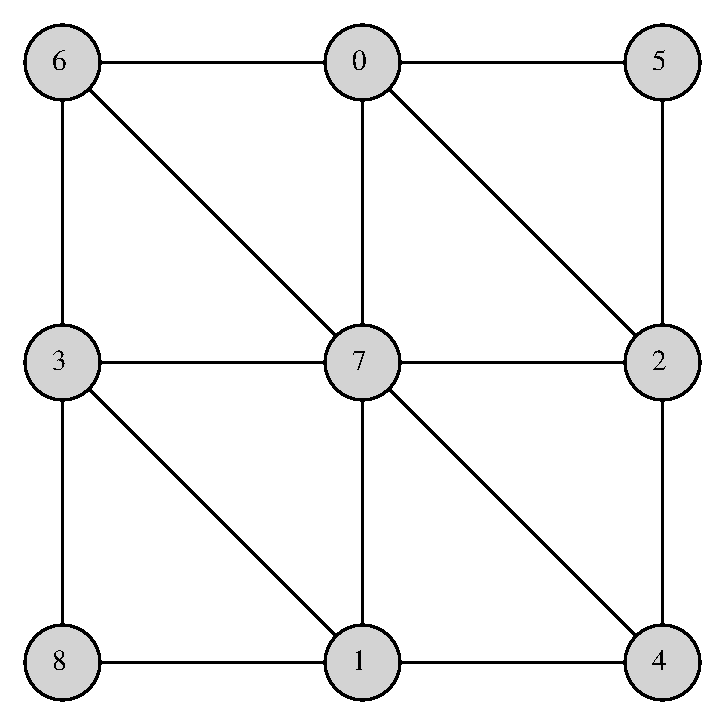
\includegraphics[scale=0.4]{./images/chapter4/w3x3-grid.eps}}}%
    \qquad
    \subfloat[Contour Tree]{{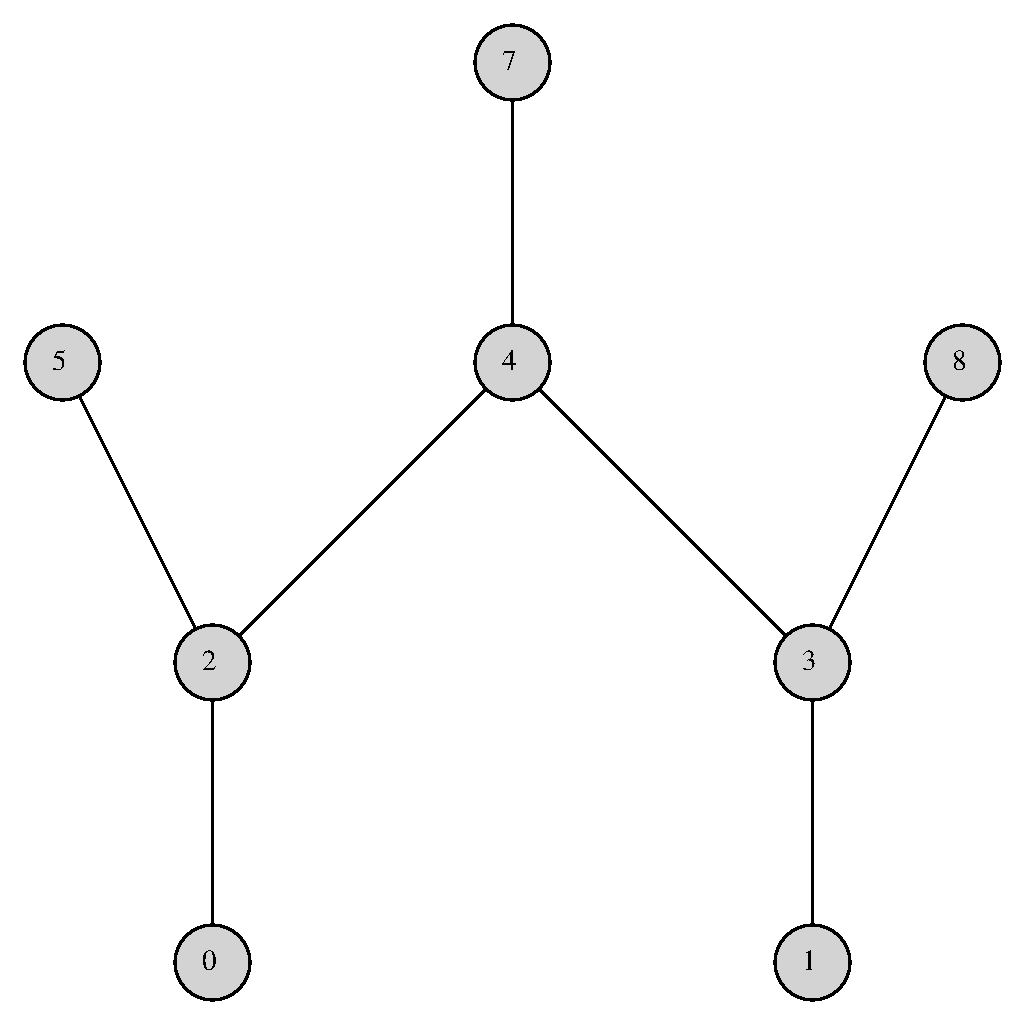
\includegraphics[scale=0.3]{./images/w3x3.eps}}}%
    \qquad
    \subfloat[Branch Decomposition.]{{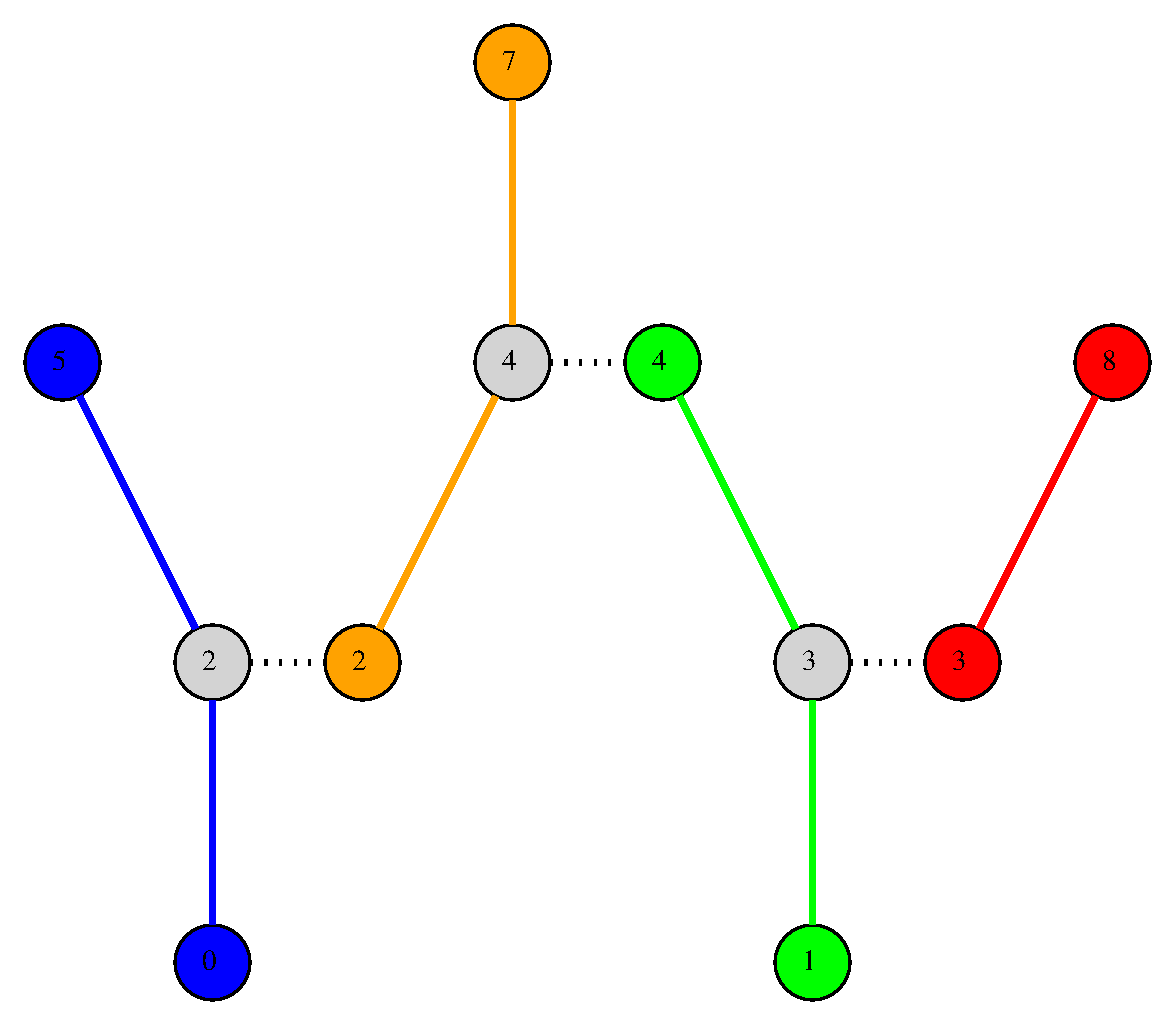
\includegraphics[scale=0.3]{./images/branch-decomposition-W3x3.eps}}}%
    \caption{Branch Decomposition of the Contour tree.}%
    \label{fig:example}%
\end{figure}


\begin{figure}[h]%
    \centering
    \includegraphics[scale=0.08]{./images/chapter4/asc-filt.eps}%
    \caption{Ascending filtration of the Simplical Complex}%
    \label{fig:filt-sc}%
\end{figure}

\begin{figure}[h]%
    \centering
    
\includegraphics[scale=0.08]{./images/chapter4/ph.eps}%
    \caption{Extended Persistence of the Simplical Complex}%
    \label{fig:filt-sc}%
\end{figure}



\subsection{Thoughts on future directions}

There are many more unansweared question on the relations of contour tree simplification and persistent homology. For example notice that the way the 0th persistence of an ascending filtration is computed is similar to how a join tree is computer. The similarity is in that joining components correspond to connected components in sublevel sets which in turn correspond to homology classes in the 0th homology. The joining of components coresponds to merging of homology classes. Consequently the persistent pairs correspond to branches in the join tree. If we instead take a descending filtration we obtain a similarity between the split tree and the persistent homology of the descending filtration. Further work can be done in showing whether the computations are equivalent formally and in translating idea from each of the frameworks to the other.

Another question is whether contour tree simplification can be expressed through through some filtration similar to persistent homology. Consider for example a simplicial mesh $M$ and its level sets $M_i$. Homology gives us to tools of identifying the connected components of the the $M_i$ by computing the 0th homology. It is possible however to somehow relate the homology classes of different level sets. This would require a sequence of the form

$$ ... \rightarrow H_0(M_i) \rightarrow H_0(M_{i+1}) \rightarrow ... \rightarrow H_0(M_{j}) \rightarrow H_0(M_{j+1}) \rightarrow ...$$

But what would the function between the homology groups be? Can me somehow induce them through function between the sublevel sets themselvs? We certainly cannot use inclusion maps because level sets are not neseted. It is worth contemplating whether this is feasble. Another question is whether it would be practical at all. Even if we do so all we will obtain is a mathematical reformulation of a problem we already have. Will that lead to more efficient algorithms or to better understanding of the subject?

We are not able to expand more on questions like these and leave them as subject for further study.

% What we have uncovered is not the complete story. There is a deeper connection between extended persistence and contour trees in general. If we look at alternative algorithms for constructing the 0th homology specifically we can see that the extended persistence of an ascending filtration is equivalent to branch decomposition of the join tree and the extended persistence is equivalent to a branch decomposition of the split tree.

% Going back to the claim made \cite{ct-branch-decomp} we see that there is truth to it if we adjust it to extended persistence and apply specifically to join and split trees. Here future questions that arise based on this fact.

% \begin{itemize}
%     \item By using the persistence pairs on other homology group we can produce split and join tree for the cycles, void, etc... We can them combine them like we combine the join and split trees for the contour. What kind of a structure does that yield?
%     \item Can we compute the contour tree directly from homology. Can we find a natural continuous function between the level sets of a filtration. Would the persistence of this sequence be equivalent to the contour tree. In higher dimensions would be equivalent to the previous point?
%     \item Who killed Laura Palmer and will the new Twin Peaks be good?
% \end{itemize}



%In this final section we will present examples for how extended persistence on the 0th homology is actually equivalent to computing join and split tree.

%*Don't know if I can prove this yet, but it probably won't be too hard. But then again it may be.*

%*Should I keep this or not?*







% @TODO Check spelling in references.



%Let us now restrict $M$ to be compact and contractable. This will ensure that the Reeb Graph of $M$ is a Contour Tree. We would like to tackle the claim made in \cite{ct-branch-decomp} that the persistent homology pairs are equivalent to branch decomposition pairs. We can immediately see that this claim is either false of ill-defined. The major reason for this is that essential homology classes do not get paired. But in the branch decomposition schemes all critical points are paired.

%There is however yet more reason to pursue this. Slightly after the paper of branch decomposition was published, there emerged a way to extend the persistent homology scheme so that all critical points get paired. Using this will allows us to directly compare it to the branch decomposition of a contour tree.




%Lastly we will not that we cannot take into account the



%Explain the claim that has been made and quote it directly.

%Show why it is flawed in the first place.

%Show why it's not equivalent to it.



%* Most of this sections will be pictures this is why it is not written up properly *

%Now let us examine the relation of extended persistence to branch decomposition. Here is an example branch decomposition of a contour tree of the following 3x3 grid dataset. It is not possible for the branch decomposition to pair the global maximum with the global minimum. There is no monotone path between them. To show that no branch decomposition of a contour tree is equivalent to the extended persistence of the dataset I will demonstrate that extended persistence necessarily pair the global minimum with the global maximum.

%*Show the extended persistence filtration of the W3x3*
%*Show the branch decomposition*


% @TODO Add quote
%As you can see these methods produce very different pairings. We will conclude that the claims made in [] are either false of not well defined. The correct way to phrase this is the following. "Our definition of persistence is quivalent to extended persistence for the join and split trees. It is not directly applicable in the case of the contour tree itself in terms of the formalism it's built on".


%It so happens that a w-structure that this dissertation is devoted to causes not only computational difficulties, but also serve as counterexamples to pose theoretical difficulties as well. To further cement statement we will us show a more general general result in the following chapter which holds for all filtrations of path-connected spaces.


%The maps in the ascending filtrations are induced via the inclusion maps between the nested spaces $M_i \subseteq M_j$  where $i \le j$. The more interesting case if between the relative homology groups. First of all the isomorphism between $H_n(M) = H_n(M, M^{c_n})$ comes from that fact that $M^{c_n} = \emptyset$ and quotienting by the empty sets leaves a group unchanged. The show where the consecutive maps come from we will give the following example.

%Let $X$ be a simplical complex, $B \subset X$ be a subcomplex of $X$ and $A \subset B$ be a subcomplex of $B$. Then we can find a natural map from $H_n(X, A)$ to $H_n(X, B)$ induced by the inclusion from $A$ to $B$. Let us write out $C_n(X), C_n(A), C_n(B)$ through their generator simplicies.

% @TODO Fix these brackets
%$$ C_n(X) = <a_1, a_2, ..., a_k, ..., a_l, ..., a_n> $$
%$$ C_n(A) = <a_l, ..., a_n>$$
%$$ C_n(B) = <a_k, ..., a_l, ..., a_n>$$


%Then the relative chains are generated by:

%$$ C_n(X, A) = <a_1, ..., a_k, ..., a_{l-1}>$$
%$$ C_n(X, B) = <a_1, ..., a_{k-1}>$$


% @TODO Show it is a chain map

%Where we can introduce a natural inclusion map $f : C_n(X, A) \to C_n(X, B)$ where $f(a_i) = a_i$ when $i < k$ and $f(a_i) = 0$ when $i \ge k$. The map $f$ is well defined as an inclusion map and furthermore it is a chain map. Chain maps induce linear maps on the homology. Therefore we obtain the map $f_* : H_n(X, A) \to H_n(X, B)$ where $f_*([\alpha]) = [f(\alpha)]$. Where the brackets denote the homology quotient classes in $H_n(X, A) \text{ and } H_n(X, B)$ respectively.

%Now let us to back to the descending filtration of $M$. We have

%Let us go back extended persistence. In the descending filtration of the relative homology we have the scenario we just described. Therefore as there is an inclusion function for between every $M^{c_i}$ and every $M^{c_j}$ where $i \ge j$ and this induces a linear map between every $H_n(M, M^{c_i})$ and $H_n(M, M^{c_j})$.

%We have developed all this mathematical machinery

%-- Give some intuition behind this.

%-- Show how this is used on an example.

%-- Give an algorithm for computing it.

%-- Explain how the algorithm is connected to the computation.

%\section{Persistent Homology and the Contour Tree}

%-- Say some general things about how we are going to relate the two and what we shall accomplish in this chapter.

%\subsection{Join and Split Trees}

%Show that the computation of the ascending filtration and descending filtration is equivalent to the join and split tree of a contractable domain.

%Show the it is equivalent to branch decomposition of the join and split tree.

%Show that extended persistence pairing are not equivalent to branch decomposition pairing. Say the paper is either wrong or had something else in mind which is not clarified well enough.

%Emerge victorious and have the plebeians chant you name in the streets. All Hail Petros all hail Petros.



% In order to produce a detailed computation of the persistent homology of a filtration we would have to compute all homology groups of all complexes and then compute all inclusion maps. Doing so by hand is cumbersome and more importantly far too lengthy. We will avoid doing it in favour of presented diagrams of the evolution of the homology classes and appeal to the reader's geometric and topological intuition to argue their correctness.

% *Let us look at the following example. Show a pretty picture and explain it*

% @TODO Why is this true?
% There is a theorem that states that the persistence digram of a filtration encodes all of the information about the persistent homology groups.
%
% *Examples*

% Finally we will describe an algorithm for computing the persistence pairs. It requires us order all of the simplices in the complex $\sigma_1, \sigma_2, ..., \sigma_n$ according to these rules \cite{ph-a-survey}.
%
% \begin{itemize}
%     \item $\sigma_i$ precedes $\sigma_j$ when $\sigma_j$ was introduced later in the filtration than $\sigma_i$
%     \item $\sigma_i$ precedes $\sigma_j$ when $\sigma_i$ is a face of $\sigma_j$
% \end{itemize}
%
% Not instead of having to compute the homology groups of all complexes in the filtration individually and then computing the induces maps we can perform the whole computation in a single matrix reduction. Let $D$ be an $n\times n$ matrix and such that.
%
%    $$
%    D[i, j] = \left\{
%        \begin{array}{@{}l@{\thinspace}l}
%            \text{1}  &: \text{if } \sigma_i \text{ is a codimension 1 face of } \sigma_j \\
%            \text{0}  &: \text{otherwise} \\
%        \end{array}
%    \right.
%    $$
%
% In other matrix $D$ is a matrix that holds the boundaries of all simplicies in a single matrix. It is called the combined boundary matrix. Now we can perform the following reduction just by column operations.
%
%
% \begin{algorithm}
% \caption{Reduce Combined Boundary Matrix}
%
% \begin{algorithmic}[1]
%
%
% \ForAll {j $\in$ \{1, 2, ..., n\}}
%     \While {$\exists j': j' < j \text{ and } low(j') == low(j) $}
%         \State Add column $j'$ to column $j$.
%     \EndWhile
% \EndFor
%
% \end{algorithmic}
% \end{algorithm}
%
% The proof of this algorithm is outlined in \cite{persistence-original}.

%
% Finally we will define what we call the persistence of a homology class.
%
% \begin{defn} The persistence of a single homology class in persistent homology that is born at time $t_1$ and dies at time $t_2$ is $t_1 - t_2$.  \end{defn}
%
% % @TODO Do this
%     There are two primary ways to visualize the persistence pairing produces by persistent homology. The first in through persistence diagrams \cite{comp-topo}. In the persistence diagrams the pairs are visualised as points in the Carthesian coordinate system above the main diagonal $y = x$. Example []. The second way is through barcode diagrams. You can see the barcode digram on fig[]. For every simplical complex in the filtration we have a number of starting lines equal to the number of generators for the homology classes. These lines feed into each other according to where the induced by inclusion homomorphism take them in the next simplical complex.
%
%
% % @TODO Return these.
%
% %\begin{figure}[h]%
%     %\centering
%     %%\includegraphics[scale=0.085]{./images/chapter4/bar-diagram.eps}%
%     %\caption{Barcode Diagram of a Filtration}%
%     %\label{fig:bar-diag}%
% %\end{figure}
%
% %\begin{figure}[h]%
%     %\centering
%     %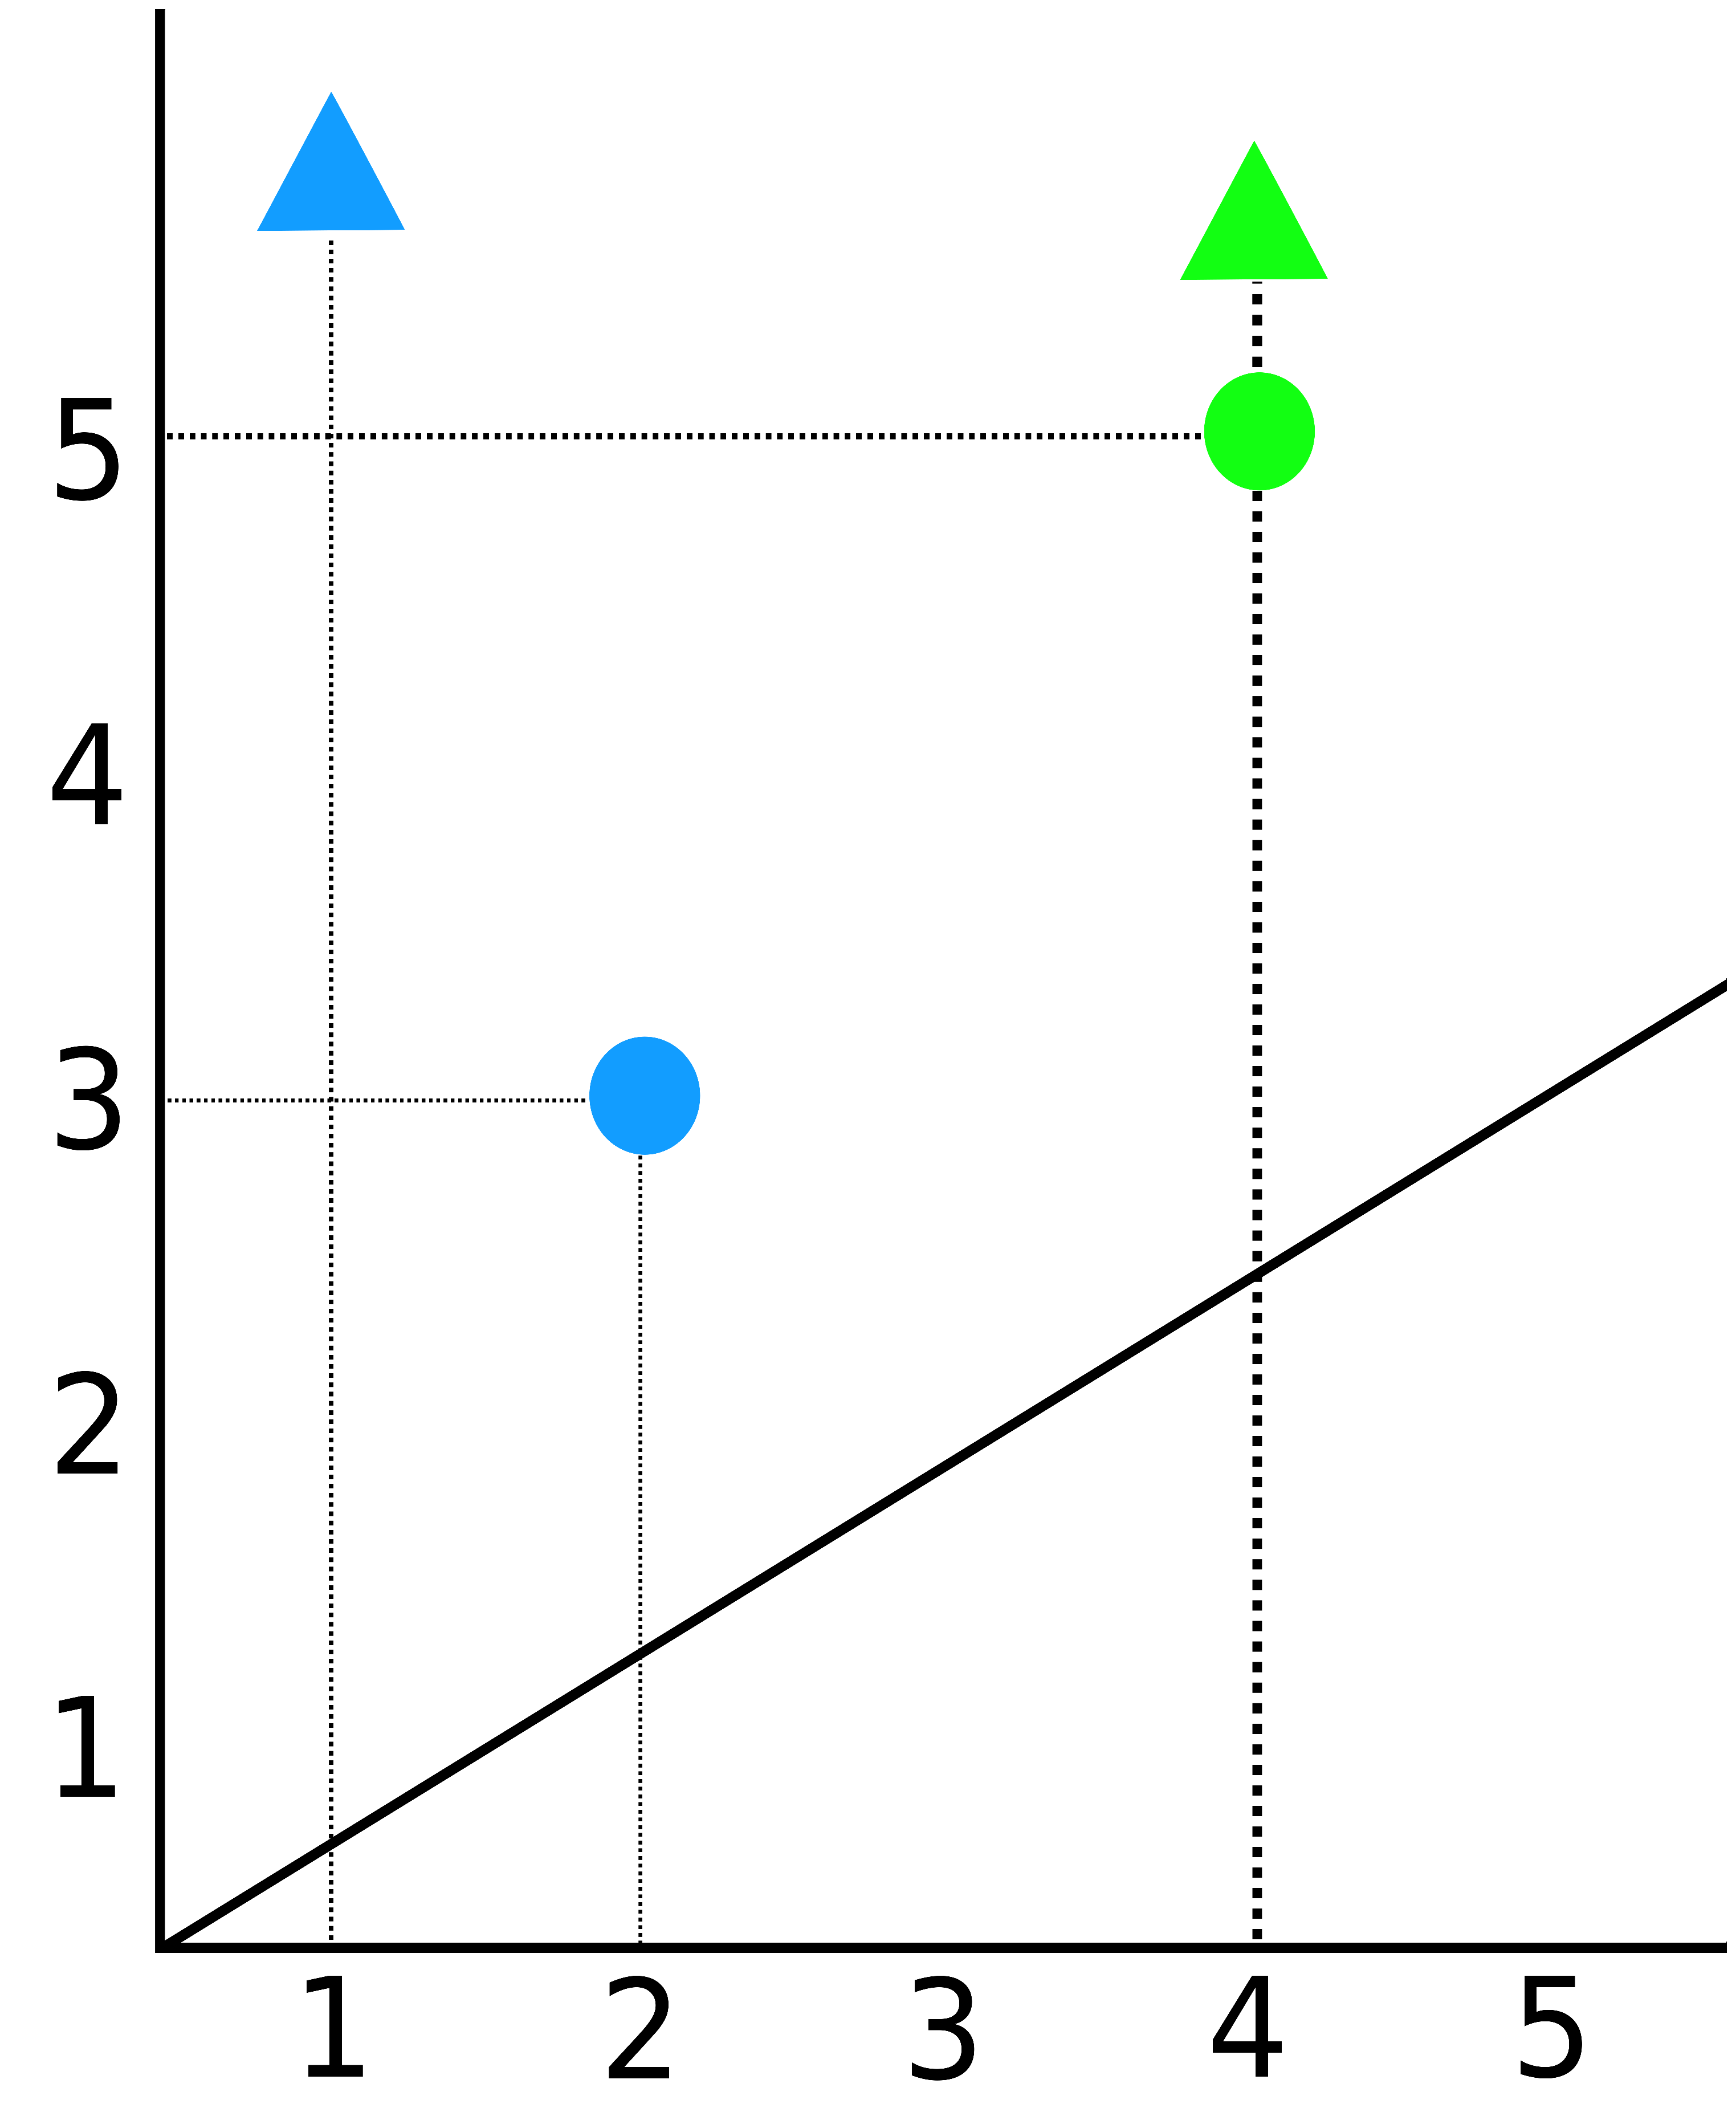
\includegraphics[scale=0.085]{./images/chapter4/diagram.eps}%
%     %\caption{Persistence Diagram of a Filtration}%
%     %\label{fig:per-diag}%
% %\end{figure}
%
%
% % @TODO Add reference
% % Furthermore when two classes merge we must choose which one survives and which one dies. By established convention [] we will use the Elder Rule. By the Elder Rule the class that was born first continues to persistent and the younger one is destroyed.
%
%
% %Here are two examples of filtrations and explanations of bar diagrams.
%
%
% %Let us now restrict $M$ to be compact and contractable. This will ensure that the Reeb Graph of $M$ is a Contour Tree. We would like to tackle the claim made in \cite{ct-branch-decomp} that the persistent homology pairs are equivalent to branch decomposition pairs. We can immediately see that this claim is either false of ill-defined. The major reason for this is that essential homology classes do not get paired. But in the branch decomposition schemes all critical points are paired.
%
% %There is however yet more reason to pursue this. Slightly after the paper of branch decomposition was published, there emerged a way to extend the persistent homology scheme so that all critical points get paired. Using this will allows us to directly compare it to the branch decomposition of a contour tree.
%
% %We will now show that computing the persistent homology of the descending and ascending filtration of $M$ is equivalent to constructing the join and split tree of $M$ respectively.
%
% %* Show that this is the case *
%
% %* SHOW EXAMPLES *
%
% % Define extended persistence.


% A natural thing to do would be to directly apply persistent homology twice. Once on the ascending and the on the descending filtration. The problem that arises is in relating the classes of the two filtrations. We cannot merge both filtrations into a single long chain because the induced maps of the two filtrations flow in different directions :
%
% $$ 0 = H_n(M_{c_1}) \rightarrow ... \rightarrow H_n(M_{c_n}) = H_n(M) = H_n(M^{c_1}) \leftarrow ... \leftarrow H_n(M^{c_{n}}) = 0.$$
%
% The direction of the arrows is accordance with the how the homomorphisms are induced. To verify this consider that $M_{c_i} \subseteq M_{c_j}$ and $M^{c_j} \supseteq M^{c_j}$ for $i \le j$. What we would like to achieve it to reach $H_n(M)$ in the ascending filtration and to start a new filtration which reduces it to the zero group by "removing" simplicies from it. We cannot do so in absolute homology because we would not have inclusion maps. We can however achieve this with relative homology. Consider the filtration:
%
% $$ H_n(M) = H_n(M, M^{c_n}) \rightarrow H_n(M, M^{c_{n - 1}}) \rightarrow ... \rightarrow H_n(M, M^{c_{1}}) = 0 $$


% @TODO By which def (end of paragraph)
% In this relative filtration the linear maps are induced by inclusions on the relative homology groups. To see this let $(M, M^{c_i})$ and $(M, M^{c_{i+1}})$ two consecutive pairs. The inclusion map from $M$ to $M$ takes the superlevel set $M^{c_i}$ in the superlevel set $M^{c_{i+1}}$ because $M^{c_i} \subseteq M^{c_{i+1}}$. By definition [] this is a simplicial map from $(M, M^{c_i})$ and $(M, M^{c_{i+1}})$ and thus induces a homomorphism between $H_n(M, M^{c_i})$ and $H_n(M, M^{c_{i+1}})$.

% The final step to complete our desired sequence is to "glue" these two filtrations together at the point $ H_n(M_{c_n}) = H_n(M) = H_n(M, M^{c_n})$. The second equality holds because $M^{c_n} = \emptyset$ and quotienting by the empty set leaves the underlying relative chain complexes unchanged. Putting this all together yields the following chain of homology groups.
%
% $$ 0 = H_n(M_{c_1}) \rightarrow ... \rightarrow H_n(M_{c_n}) = H_n(M) = H_n(M, M^{c_n}) \rightarrow ... \rightarrow H_n(M, M^{c_{1}}) = 0.$$
%
% % @TODO Is that really what a close subcomplex is?
%
% This augmented filtration justifies the pairing of essential classes according to the intuitive understanding we obtained from example []. The only issue is that the relative homology groups are difficult to interpret on their own. To aid our comprehension of what exactly occurs in the relative filtration we shall employ the Excision Theorem where $H_n(M, M^{c_i}) = H_0(M / M^{c_i}, pt) = \overset{\sim}{H}_0(M / M^{c_i})$ where $M^{c_i}$ is a closed subcomplex of $M$ as required for all $i \in \{1, 2, 3, ..., n\}$.
%
% * Take a look at example how the complex is built and the how it unwinds itself *
%
% 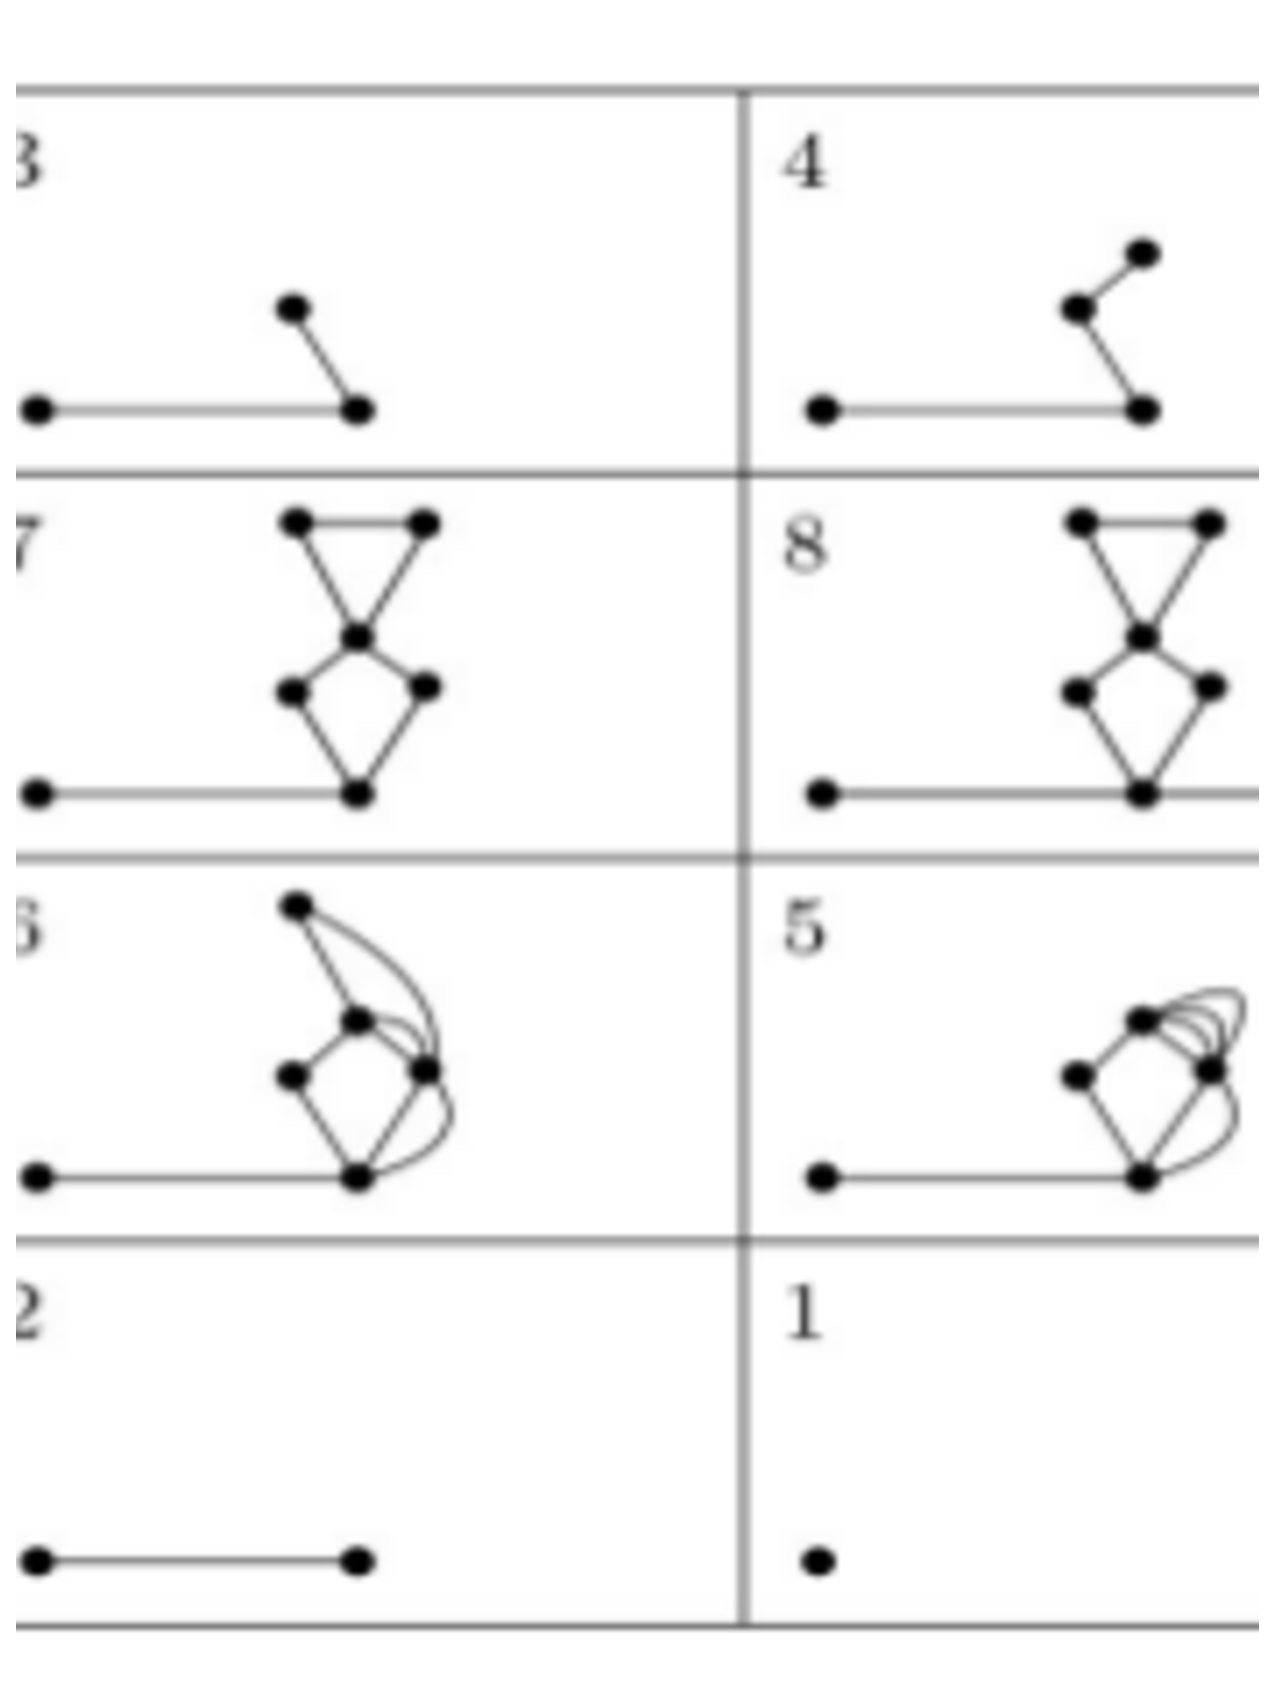
\includegraphics[scale=0.2,center]{./images/extended-ph.eps}


% Let us unpack the claim piece by piece. Firstly the paper only redefines how the persistence of the branches is computed and branches are pair of critical points. Therefore for this to be equivalent to the persistence pairs, both methods must  produce equivalent pairs. It is clear from this definition that the actual persistence pairings stay the same, we only compute the persistence value in a different way. What we will aim to show is that the pairings produced by persistent homology are in themselves different from the pairings produces by branch decomposition. After this it will not matter how the actual persistence of branches is computed as they are fundamentally different things. Lastly the paper claims that the branch decomposition definition differs from persistent homology in that "it takes into consideration the topological obstructions.". It is not clear exactly what the authors meant by "topological obstructions". These obstructions are not defined in the paper nor in subsequent publications. This does not stop us from working with the definition because we will demonstrate a second way in which persistence differs from branch decomposition.

% The first major difference we can find comes from the fact that persistent homology as it was originally defined does not pair all critical points. As we discussed previously the pairings of essential homology classes are not defined because they never die in the filtration. In the case of contour trees we will be dealing will simply connected contractable domains. Such domains have a single connected component and therefore have exactly one essential homology class in the 0th homology. This is the class that is born at the global minimum, or the first simlicial complex in the filtration. In branch decomposition on the other hand all critical points are paired.

% This is already of major difference between the two. Furthermore the paper on branch decomposition clearly cites the original paper for persistent homology and not the subsequence paper on extended persistence where this issue is remedied. In fact it cannot reference that paper. The branch decomposition paper has been published in January of 2004 and the paper that clearly defines Extended Persistence as such has been published in January of 2009 \cite{persistence-extended}. There is however more to this story. The concept of pairing critical points unpaired by persistence goes further back than the 2009 paper and can be traced to the paper \cite{extreme-elevation} which was also published in January of 2004. The paper outlines the initial concept of extended persistence in the specific case of 2-manifolds embedded in $\mathbb{R}^3$. This means that the idea of pairing all critical points was present when the claim was made. All of lets us the take this a step further. We will now test whether branch decomposition is equivalent to extended persistence.

% We will demonstrate that they are not with a small counter example. This counter example will show that at least one pair in both is necessarily different. In contour trees where the global minimum and the global maximum are not connected via a monotone path branch decomposition cannot by definition pair them as the endpoints of a branch. Extended persistence on the other hand does pair them as the global maximum is the first class in the descending relative filtration that is homologous to the essential class born at the global minimum. To reduce the stress caused by the reader's feverish anticipation of this counter example we will foreshadow that it is a contour tree with a w-structure. This w-structure is what separates the global minimum from the global maximum.

%
% \subsection{Extended Persistence on Path-Connected Domains}
%
% The final step we take on this journey will be to prove the following original and more general result.
%
% \begin{prop} In the extended persistence of filtration a Morse function with a Path-Connected domain the global minimum pairs with the global maximum in the 0th homology \end{prop}
%
% \begin{proof}
%     Let $M$ be a Path-Connected domain and let $M_1 \subseteq M_2 \subseteq ... \subseteq M_n$ be a filtration of $M$. This filtration induces etended persistence
%
% $$ 0 = H_0(M_{c_1}) \rightarrow ... \rightarrow H_0(M_{c_n}) = H_0(M) = H_0(M, M^{c_n}) \rightarrow ... \rightarrow H_0(M, M^{c_{1}}) = 0.$$
%
% As $M$ is Path-Connected it has one path-connected component and therefore $H_0(M) = H_0(M_0) \simeq  \mathbb{Z}_2$.  Our aim here will be to show that all of the $H_0(M, M^{c_i})$ are trivial. This will mean that the single homology class that exists in $H_0(M)$ will die at $H_0(M, M^{c_n})$ which is exactly the global maximum.
%
%
% % @TODO Define Excision
% % @TODO  Add the thing where this holds - H_n(M / M^{c_i}, pt) = \overset{\sim}{H}_n(M / M^{c_i})
% As a corollary of the Excision Theorem we have that
%
% $$H_0(M, M^{c_i}) = H_0(M / M^{c_i}, pt) = \overset{\sim}{H}_0(M / M^{c_i})$$
%
% where $pt = M^{c_i} / M^{c_i}$.
%
% Now let us explore the reduced homology of the topological space $M / M^{c_i}$. We will show that is it path-connected and therefore the reduced homology is trivial.
%
%
% % @TODO Add quote
% By definition $M$ is path connected. Consider the function $\pi: M \to M/ M^{c_i}$ that takes a point to it's equivalent class. By point set topology [] we know that $\pi$ is continuous. We can also infer that $\pi$ is surjective. Indeed there there is no equivalence class that no point maps to. Furthermore the continuous image of a path connected is connected by []. As we have that $M$ is path-connected therefore $\pi(M) = M / M^{c_i}$ is path-connected.
%
% By [] we have that $H_0(M / M^{c_i}) = \mathbb{Z}_2$ and by [] that $H_0(M / M^{c_i}) = \overset{\sim}{H}_0(M / M^{c_i}) \bigoplus \mathbb{Z}_2$
%
% We can conclude that $H_0(M, M^{c_i}) = \overset{\sim}{H}_0(M / M^{c_i}) = 0$
%
% Therefore the map induced by the inclusion of the pairs $(M, \emptyset) \to (M, M^{c_n})$ will map the essential homology class of $H_0(M_n)$ to zero. This mean that the global minimum pairs with the global maximum.
%
% \end{proof}
%
% Following this proposition we can only conclude that in any contractable domain with a w-structure that separates the global minimum with the global maximum branch decomposition is not the same as extended persistence.

\chapter{Empirical Study}
\label{chapter7}

In the final chapter we will suplement our theoretical ivestigation of the w-structures with an empirical study. The goal of this study if twofold. Firstly it is to verify the theoretical claims we have made on the correctness and running time of the w-diameter algorithms we developed. This will be done by implementing and testing them on a range of diverse datasets. The second goal and most important goal of the empirical study is to analyse the w-structes that are present in contour trees of real life data sets using the w-diameter algorithms we've implemented. We will conclude the chapter with a discussion on the future directions this empirical study can take.

\section{Algorithm Implementations}

For the purpose of conducting the empirical study we implemented all three w-diameter algorithms we developed in Chapter []. Those are the brute force algorithm (NxBFS), the 2xBFS and DP algorithms.  We implemented the brute force algorithm by running the modified version of 2xBFS from every vertex in the tree and outputting the largest w-path we found. The implementation of the 2xBFS algorithm was based entirely on the pseudocode we provided in Chapter []. Initially we made an recursive implementation of the DP algorithm based on the pseudocode we provided in Chapter []. This approach was not efficient enough because the recursion added a substantial amount of overhead in large data sets. We resorted to converting our recursive version to an iterative one.

When converting a dynamic programming algorithm from a recursive to an iterative solution one first identifies all base case subproblems and solves them. Afterwards one works their way up to subproblems that depend only on the base case solutions and solve those. This process is repeated until all subproblems are solved. In our particular example the base cases are the leaves of the tree. The subproblems that depend on those are for all vertices whose distance from a leaf is one. Once those are solved we move on to vertices whose distance from a leaf is two and so on. In order to make sure that we have solved the subproblems for all children of vertex we first root the tree using standard BFS. The root of the tree can be any vertex. Using the BFS we not only assing parrents to all vertices, but we also rank them based on their distance from the root. By processing vertices from furthest to the root we ensure that the subproblems of any vertex are solved for because its children have a bigger distance. In order to solve a subproblem at a vertex we can use the code we have provided in the backgracking part of the DFS in the pseudocode in Chapter [].

Finally we also implemented the serial contour tree algorithm as it is described in []. The reason for doing so is that we needed to modify its output so that we can format the input an appropriate way for our tree diameter algorithms. All four algorithms we devloped were written in C++ and their source code can be found in their github repository [].

\section{Data sets Overview}

Before proceeding to describe our testing methodology we will first elaborate on the types of data sets we will be using throughout our tests. The first type of data sets we will use are randomly generated height trees. In testing the correctness and running time of the w-diameter algorithms we would ideally like to run them on as many different data sets as possible in order to confirm our theoretical claims for all of them. Generating height trees randomly will allows us to produce "new" data sets for testing on demand. We will now describe what algorithm we use for doing so.

Starting with a disconnected graph $G$ with $n$ vertices we continually generate pairs of vertices $u, v$ in with labels in the range $\{1, 2, ..., n\}$. If adding the edge $uv$ to the graph does not create a cycle we keep the edge. If it does create a cycle we discard it. We continue generating edges randomly untill the $G$ is fully connected. Upon reaching this point $G$ will be a connected graph with no cycles. This is exactly the definition of a tree. In order to produce valid height trees we assign a random height to each of the vertices of the tree. In order to detect of whether adding an edge produces a cycle we use the union-find data structure to keep track of which connected components vertices belong to. We add an edge between two vertices only when they belong to a different connected component and then merge the two components together.

The second type of data sets we will use is real life data taken from the GTOPO30 data set. GTOPO30 [] is a digital elevation model of the world. The dataset is a two dimensional data grid containing the elevation of points on Earth with a resolution of approximately one kilometer. The primary use of this data set will be for the generation of a contour tree of the data and analysing the pesent w-structures. GTOPO30 however is far to large for us to handle without specialised hardware. This is why we have taken several smaller subsets of GTOPO30 provided to us by Dr. Hamish Carr.

We have chosen for our data sets to be mountaneous regious due to their more complex topographic structures. The data sets we will use are named vanc (18x21) ,vancouverSWSW (25x49) ,vancouverSWNE (25x50), vancouverSWNW (25x50), vancouverSWSE (25x51), vancouverNE (49x99), vancouverNW (49x100) , vancouverSE (50x99), vancouverSW (50x100), icefield (240x240), pukaskwa (551x1600), gtopo30w020n40 (6000x4800). The vanc and all vancouver data sets are taken from the North Shore Mountains that overlook Vancouver in British Columbia, Canada. The data set pukaskwa is taken from the Pukaskwa National Park located south of the town of Marathon, Ontario, Canada. The data set icefields is taken from []. Finally gtopo30w020n40 is the data set that contains all other data sets.

\section{W-detector Algorithms}

We have already provided details on the implementations of the three w-diameter algorithms we devoloped in Chapter 3. These are the NxBFS algorithm (brute force approach), 2xBFS (running modified Breadth First Search twice) and DP (dynamic programming based approach). In this section we will use their implementations to empirically test whether our claims on their correctness and running time are correct.

The first test we will present is on the correctness of all three algorithm. The major issue we encountered in this test is that all three algorithm solve a problem that to our knowledge has not been been considered extensively in the past. The only way to establish ground truth on their output is to manually inspect the w-diameter of a height tree. This is neither reliable nor scalable to height trees with more than a few dosen vertices.

To overcome this issue we opted for using the output of the NxBFS algorithm as ground truth. The reasoning behind this is that it is the most straighforward to implement and that its correctness is a trivial consequence of its formulation. What this leads us to believe is that it is the most reliable of the three. Even so, a further complication arises in that the NxBFS algorithm's running time is quadratic and not linear like 2xBSF and possibly DP. This leaves us unable to use this methodology for large enough trees where the NxBFS algorithm's computation simply scales to unreasonable time. This is why we have limited ourselves to only testing correctness for trees of up to 10,000 vertices. For this test we have used the following testing methodology:

\begin{itemize}
    \item Generate a random tree.
    \item Run all three algorithms on the tree.
    \item Check whether the output of DP and NxBFS are the same and if the output of 2xBFS is within two of their output.
\end{itemize}

We then used this methodology to run tests on one thousand trees of sizes $50$, $100$, $250$, $500$, $750$, $1000$, $2500$, $5000$, $7500$, $10000$ resulting in $10000$ individual tests alltogether. The output of all tests was in line with what we predicted in Chapter 3. The algorithms DP and NxBSF had identical output and the output of the 2xBSF algorithm was no less than two of their output. These results strengthen our belief in the correctness of all three algorithms.

The second test we will perform is on the running time of the algorithms. In this test we will separate the algorithms in two groups. The first group will consist of NxBFS and the second group of 2xBFS and DP. We have separated them because we expect the running time of NxBFS to be quadratic, 2xBFS to be linear, DP to be close to linear and we want to results from each group to be comparable. The results from testing the NxBSF algorithm were completely as expected. You can see the running time on Figure []. *I willl add them if I have space otherwise not*

The tests of the 2xBFS and DP algorithm suprised. The test consisted of generating five tree on vertices in the range $\{5000, 10000, ..., 200000\}$, running both algorithm on all five trees and plotting the average running time on Figure [].

\begin{figure}[h]%
    \centering
    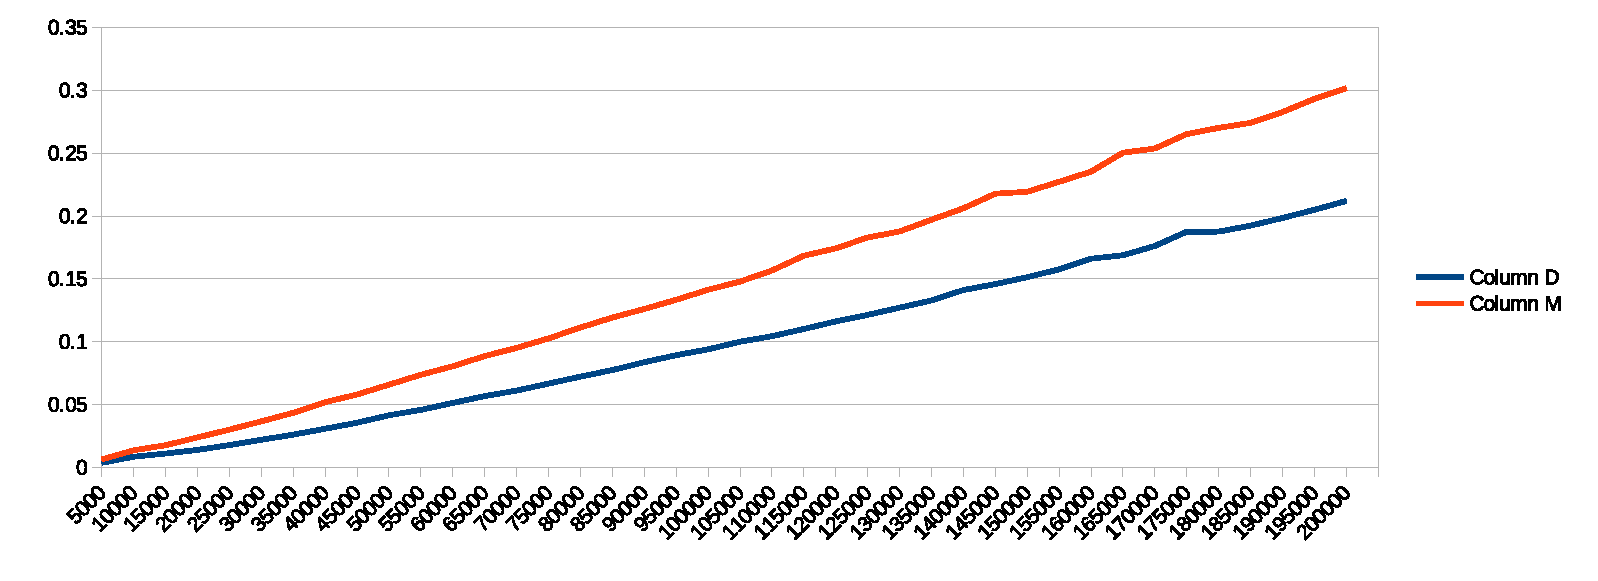
\includegraphics[center, scale=0.6 ]{./images/running-time-new.eps}
    \caption{Running time of 2xBFS (blue) and DP (red) on randomly generated trees. }%
    \label{fig:case1.1}%
\end{figure}

Both algorithms appear to fit a line almost perfectly. This is reason enough to believe that the peformance of both scale linearly with randomly generated data. This comes as no suprise as regards to the 2xBSF algorithm. What is interesting to see is that the DP algorithm's performance scales linearly as well. We must note however that these tests use randomly generated trees and are a very limited sample so this trend may not hold for all possible inputs and especially for larger trees. Despite these reservations this test gives credibility to the claim we made in the Chapter 3 that the DP algorithm has potential for good practical performance.

% Our next test was again on the running time of the algorithm but on the real data sets. The tests were run on the augmented contour tree of the datasets.

The next test we made was on the running time of the algorithms on the GTOPO30 data sets. We ran the tests for both the augmented and unaugmented contour trees and recorded how many time times faster 2xBFS is than DP in the Factor column of the tables.

% 25.60 Товарителница 800044202201

\begin{center}
\begin{tabular}{l*{6}{c}r}

Dataset            & Vertices        & 2xBFS              & DP                   & Factor \\
\hline
vanc	           & 378	         &0.000413	          & 0.000497	         &1.20    \\
vancouverSWSW	   & 1225	         &0.000918	          & 0.002317	         &2.52    \\
vancouverSWNE	   & 1250	         &0.000937	          & 0.001858	         &1.98    \\
vancouverSWNW	   & 1250	         &0.000798	          & 0.002454	         &3.08    \\
vancouverSWSE	   & 1275	         &0.001009	          & 0.00204	             &2.02    \\
vancouverNE	       & 4851	         &0.003637	          & 0.005493	         &1.51    \\
vancouverNW	       & 4900	         &0.002893	          & 0.005612	         &1.94    \\
vancouverSE	       & 4950	         &0.002958	          & 0.005863	         &1.98    \\
vancouverSW	       & 5000	         &0.002795	          & 0.005658	         &2.02    \\
icefield	       & 57600	         &0.036430	          & 0.066978	         &1.84    \\
pukaskwa	       & 881600	         &0.520608	          & 0.962897	         &1.85    \\
gtopo30w020n40	   & 28800000	     &19.103233	          & 34.427916	         &1.80    \\

\end{tabular}
\end{center}

The results from this test are completely in line with what we obtained from the previous test. As you can see the linear relationship between the two still holds. DP is within the range of 1.2 - 3 times slower than the 2xBSF algorithm. In our next test we tested the same data sets, but we computed their unaugmented contour tree.

\begin{center}
\begin{tabular}{l*{6}{c}r}
Dataset                & Vertices                    & 2xBFS                             & DP                    & Factor \\
\hline
vanc	               & 29    	                     & 0.000136	                         & 0.000057	              & 0.42  \\
vancouverSWSW	       & 58   	                     & 0.000372	                         & 0.000127	              & 0.34  \\
vancouverSWNE	       & 148  	                     & 0.000355	                         & 0.000237	              & 0.67  \\
vancouverSWNW	       & 88   	                     & 0.000412	                         & 0.000163	              & 0.40  \\
vancouverSWSE	       & 109  	                     & 0.000351	                         & 0.000193	              & 0.55  \\
vancouverNE	           & 946    	                 & 0.001888	                         & 0.001730	              & 0.92  \\
vancouverNW	           & 911    	                 & 0.001505	                         & 0.001292	              & 0.86  \\
vancouverSE	           & 782    	                 & 0.001466	                         & 0.001107	              & 0.76  \\
vancouverSW	           & 380    	                 & 0.001756	                         & 0.000802	              & 0.46  \\
icefield	           & 7655  	                     & 0.013704	                         & 0.010280	              & 0.75  \\
pukaskwa	           & 65826 	                     & 0.183262	                         & 0.100899	              & 0.55  \\
gtopo30w020n40	       & 2436622 	                 & 6.609592	                         & 3.742080	              & 0.57  \\

\end{tabular}
\end{center}


The results here are quite suprising and they requried us to double check the test multiple time. On the outlook it seems that the two algorithm had exchanged their positions. For all these unaugmented contour trees DP is 1.2 - 3 times faster than the 2xBFS algorith. We are curious to know why this is the case. The difference between the augmented and the unaugmented datasets is that in the unaugmented datasets all vertices of degree two are removed. It would appear to be the case that such vertices are processed faster by the 2xBFS algorithm and the DP algorithm has some overhead associted with them.


*I'll leave this paragarph and expand it if I have extra space*. Finally we would like to present a special case where the DP algorithm perform poorly. This case is for trees with vertices of high degree. Take for example a type of tree called a start Figure []. The doubly nested loop of the algorithm causes quadratic performance. To test this we generated a number of star like trees and compared the performance of NxBFS and DP.

% As we can see the results are again consistent with what we had with the random data sets.
%
% Except for gtopo30w020n40 where for some reason it's the other way around!!!
%
% Maybe it's the number of leaves? But it doesn't seem that way.


\section {Dataset w-diameter analysis}

In this section we will examine w-structures present in real data sets. Our goal is to demonstrate that they not only pose a theoretical difficulty, but also appear in real data and hinder performace. In this study we will run our w-diameters algorithm on the mountain range data taken from GTOPO30. We will compare the w-diameters of the contour trees of the data sets with the diameters of the unaugmented and the augmented contour trees. We will demonstrate that w-diameter of a contour tree is a better theoretical upper bound on the time complexity of the parallel contour tree algorithm than either of the diameters. Secondly we will compare the w-diameter of a contour tree with the number of iterations that are need to collapse the join and split trees. We hope to find a correlation between the two and shed light on whether it is the largest w-structure in a contour tree that prevents logarithmic in the merge phase. We have taken the number of iterations by running an implementation of the parallel contour tree algorithm based on [] provided to us by Dr. Hamish Carr [].

\begin{center}
\begin{tabular}{l*{6}{c}r}
Dataset             & 2BFS  & DP    & NBFS    & Aug Diameter  & Diameter  & Iterations\\
\hline
vanc                & 2     & 2     & 2       & 311           & 11        & 2  \\
vancouverSWSW       & 2     & 2     & 2       & 845           & 17        & 3  \\
vancouverSWNE       & 5     & 5     & 5       & 423           & 34        & 4  \\
vancouverSWNW       & 3     & 3     & 3       & 712           & 23        & 3  \\
vancouverSWSE       & 3     & 3     & 3       & 759           & 30        & 3  \\
vancouverNE         & 4     & 5     & 5       & 1338          & 128       & 5  \\
vancouverNW         & 5     & 5     & 5       & 1456          & 98        & 5  \\
vancouverSE         & 6     & 6     & 6       & 1306          & 118       & 5  \\
vancouverSW         & 4     & 4     & 4       & 1977          & 48        & 4  \\
icefield            & 7     & 7     & 7       & 12280         & 886       & 6  \\
pukaskwa            & 180   & 180   & N/A     & 374866        & 1046      & 94 \\
gtopo30w020n40      & 8     & 8     & N/A     & 15766966      & 305290    & 8  \\

\end{tabular}
\end{center}

%@TODO Remove the equiv
The first infrence we can make is about the pukaskwa data a set. Both the w-diameter and number of iterations are drastically bigger than all of the other data sets. If logarithmic collapse was taking place in the merge phase of the construction of the contour tree of pukaskwa than we would expect that to take $log_2(881600) \equiv 19$ iterations. Instead it takes $94$ iterations. This is consistent with the w-diameter of the data sets. Indeed $94$ is almost twice as less as the w-diameter. If we consider that the algorithm can process two branches on oposite sides of the w-diameter at a time it makes sence that it should take twice as less iterations for the collapse if it were w-diameter that is causing it.

Secondly we can confirm that the w-diameter in almost all of the data sets (except for vancouverSWSW) is bigger than or equal to the number of iterations. This leads us to believe that there may be some correlation between the two. In the case of pukaskwa we have already given an interpretation of this corelation. By that reasoning we would expect that in other data sets the w-diameter to be twice as much as the number of iterations. This is not the case and this may very well be due to how different w-structures interact in the merge phase. This is something we have not investigated as we only record the largest w-structure.

% Another interesting thing to note is that pukaskwa is a subset of the gtopo30w020n40 dataset and yet it's w-diameter is far smaller. This proves that the contour trees of subsets of data need not have a smaller w-diamete. Strangely enough as a consequence of this subsets of data may not be faster to compute. This has

Fillay we turn our attention to the diameter of the augmented and unaugmented contour trees. The parallel contour tree algorithm currently uses those as an uppen bound on the time complexity of the merge phase []. We have already shown theoretically that the w-diameter of a height tree is necessarily smaller than its diameter. This empirical study demonstrates the practical relevance of this findind. In the most extreme example, that of gtopo30w020n40, the w-diameter of the augmented contour tree is 1,970,870 times smaller than its diameter. For all practical intents and purposes this is a staggering difference. If the w-diameter of that data sets were equal to the actual diameter, than we would expect the merge phase to take a far larger number of iterations and severly limit the available parallelism in it.

% \section{Generating W-Structures Manually}
%
% % We can generate them via ridges and valleys.
% The next step we shall take in improving our understanding of the w-structures empirically will be to devise a way of creating data sets whose contour trees have an arbitrarily large w-diameter. In order to do so we took an approach of exhaustive enumeration. We limited ourselves to two dimensional data sets of dimension 3x3. Enumerating larger two dimensional data sets or almost any three dimensional data sets would not be feasible due to the number of permutations required. We created a program that generated all permutations of the numbers $1, 2, 3, 4, 5, 6, 7, 8, 9$ and arraged them in a 3x3 grid. After genrating all permutation we computed their contour tree and inspected the ones with maximum w-diameter. In our findings we discovered that there is a particular pattern in two dimensional data grids that can exploited to generate arbitrarily large w-structures. As an example consider our familiar simplicial mesh and contour tree on Figure [].
%
% % Here is an example data set and it's contour tree.
%
% % The data set consists of ridge and valleys.
%
% % This led us to find a pattern. Consider the data set.
%
% % \[
% %  \begin{matrix}
% %   1 & 0 & 1 \\
% %   0 & 1 & 0 \\
% %   1 & 0 & 1
% %  \end{matrix}
% % \]
%
%
% \begin{figure}[h]%
%     \centering
%     \subfloat[Simplicial Mesh]{{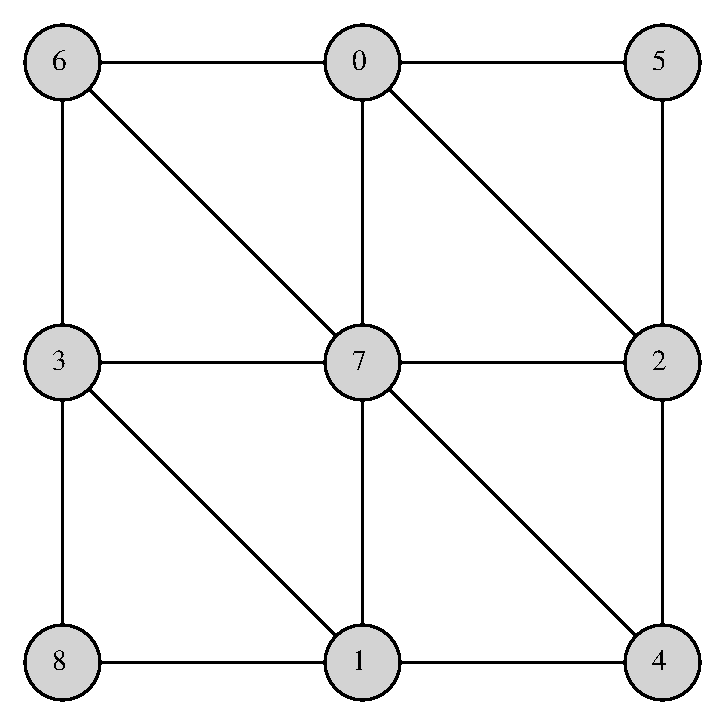
\includegraphics[scale=0.4]{./images/chapter4/w3x3-grid.eps}}}%
%     \qquad
%     \subfloat[Contour Tree]{{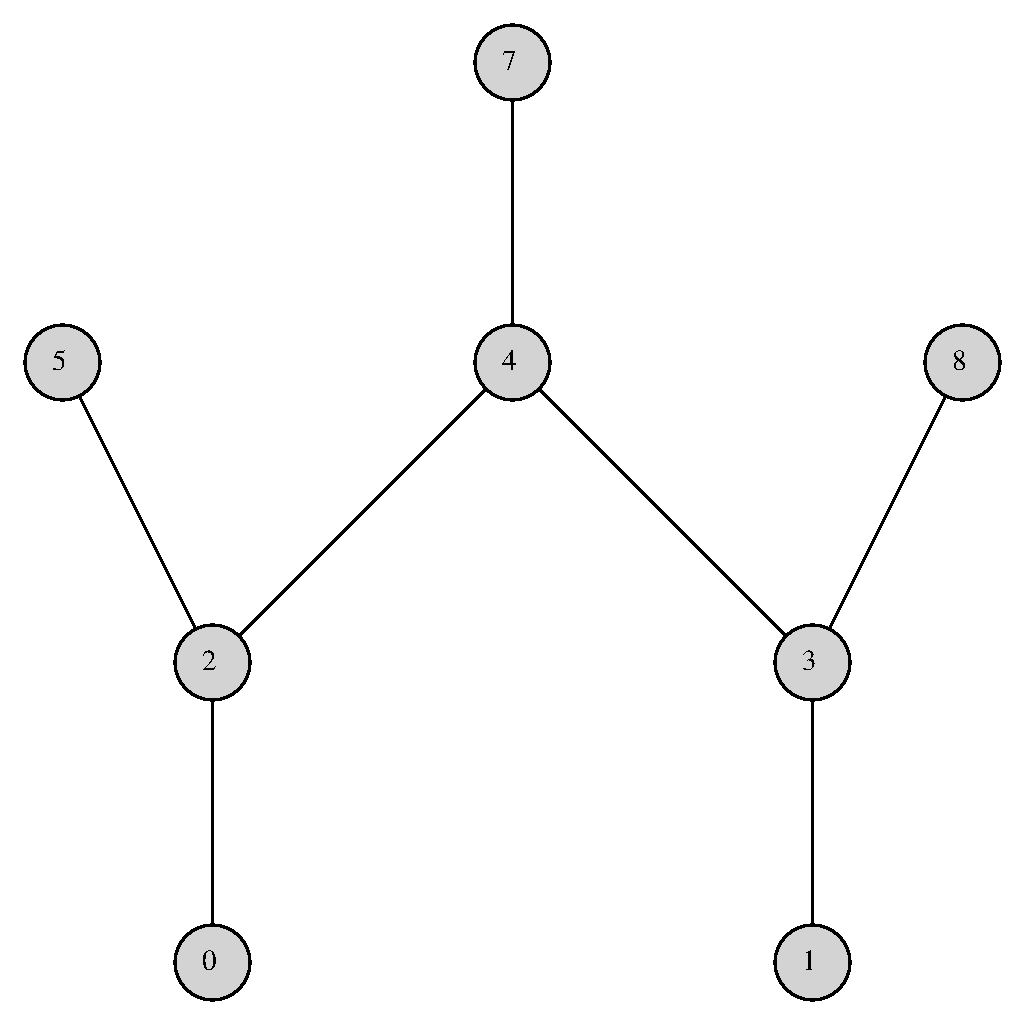
\includegraphics[scale=0.3]{./images/w3x3.eps}}}%
%     \caption{Simplicial Mesh of a Contour Tree}%
%     \label{fig:example}%
% \end{figure}
%
% The pattern in this simplicial mesh that is responsible for the w-diameter of three is a series of diagonal ridges and valleys. We can describe it like so:
%
%
% \[
%  \begin{matrix}
%   1 & 0 & 1 \\
%   0 & 1 & 0 \\
%   1 & 0 & 1
%  \end{matrix}
% \],
%
% where the ones represent vertices with heights bigger than the vertices labeled as zero and the relative height between of vertices with label one (or zero) does not matter. In order to expand the w-diameter by one we must extend the data set with an additional column.
%
% \[
%  \begin{matrix}
%   1 & 0 & 1 & 0 \\
%   0 & 1 & 0 & 1 \\
%   1 & 0 & 1 & 0
%  \end{matrix}
% \]
%
% The resulting contour tree of this data set would be.
%
% \begin{figure}[h]%
%     \centering
%     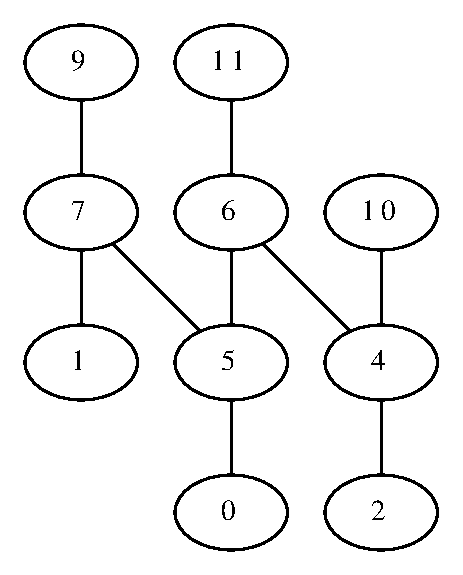
\includegraphics[center, scale=0.6 ]{./images/tree.eps}
%     \caption{Contour Tree of Dataset [] }%
%     \label{fig:case1.1}%
% \end{figure}
%
% After extending the data set for example to a 3x10 data set we obtain the following:
%
% \[
%  \begin{matrix}
%   1 & 0 & 1 & 0 & 1 & 0 & 1 & 0 & 1 & 0 \\
%   0 & 1 & 0 & 1 & 0 & 1 & 0 & 1 & 0 & 1 \\
%   1 & 0 & 1 & 0 & 1 & 0 & 1 & 0 & 1 & 0
%  \end{matrix}
% \]
%
% This 3x10 data set results in a contour tree with a w-diameter of ten on Figure [].
%
% \begin{figure}[h]%
%     \centering
%     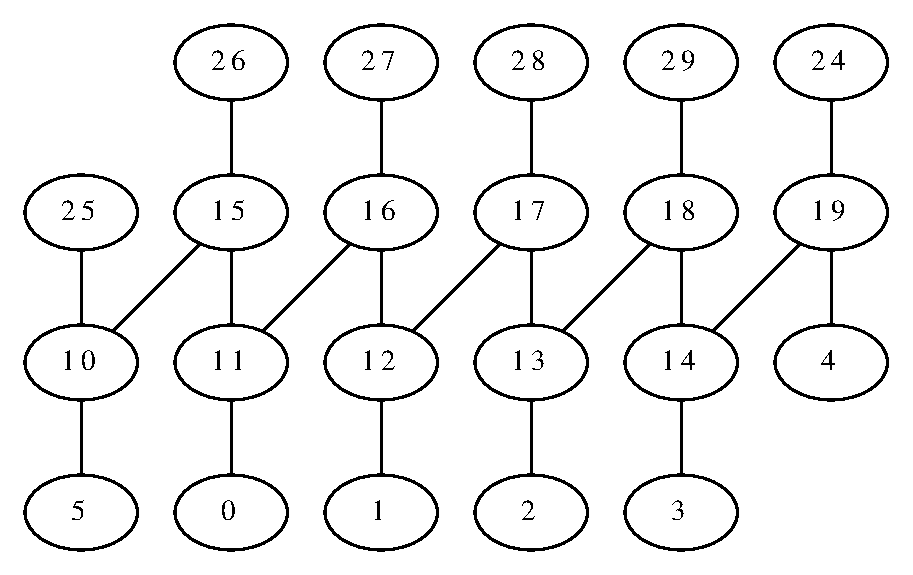
\includegraphics[center, scale=0.6 ]{./images/tree10.eps}
%     \caption{Contour Tree of Dataset [] }%
%     \label{fig:case1.1}%
% \end{figure}


% Can be obtain the w-diameter from raw data?

% Can we generate them in other ways?




% In this chapter we will study the w-structures empirically by implementing the algorithms that we can developed in Chapter \ref{chapter2} and using them to analyse real world data sets. The reason for studying them in practise is to learn more about them and explore how exactly they slow down computation. To accomplish this we will set two primary objectives. Firstly to correlate the iterations needed to collapse the contour tree in the merge phase of the algorithm with its w-diameter. This aims to give strength to the hypothesis that the w-structures do slow down computation in practise. Secondly to demonstrate that w-structures are found in real world data and do appear more abundantly as the size of datasets increases.
%
% In addition to out primary objectives there are some additional topics, related to the empirical study, that will be explored
%
% \begin{itemize}
%     \item Description the implementation of all used algorithms.
%     \item Demonstration of the running time of the implementations of the algorithms.
%     \item Correlating iterations for collapse with w-diameter of randomly generated tree.
%     \item Determining the smallest 2-dimensional grid dataset that exhibits a w-structure.
%     \item Discussion on the kinds of structures in raw data that produce w-structures in the contour trees.
%     \item Discussion on whether it is possible to determine the w-diameter of a datasets without computing it's contour tree beforehand.
%     %\item Exploring the statistical distribution of w-structures in randomly generated trees.
% \end{itemize}

%The first step to overcoming a problem is to learn about it. We .
%As a result of this study we will be able to shed light on the practical obstacles that the w-structures pose.

% For the purpose of the empirical study we implemented all three w-diameter algorithms we developed in the previous chapter. Those are the brute force algorithm, the 2xBFS and DP algorithms. In order to produce the contour trees of real life data sets we also implemented the serial version of the contour tree algorithm that is based directly on \cite{carr-masters}. To test our implementations for correctness we required the generations of more data sets than we had. This is why we have also written three small utility programs. One generates randomly populated data grids of size $n \times m$, the second generates random trees on $n$ vertices and lastly one that generates all $n \times m$ permutations of data grids populated with the numbers from $1$ to $n \times m$.  All algorithms were implemented in C++ and all algorithms are serial.
%
% The first algorithm that we implemented was the algorithm for computing the contour tree. To keep the implementation of this algorithm straightforward we have opted for working with two dimensional data sets only. To ensure the correctness of the implementation we have ran the code against code provided by Dr. Hamish Carr that implements the same algorithm. We have found that the two implementations produce the same output for all data sets we have tested - both from real data and random data.
%
% For the brute force algorithm and the 2xBFS algorithms we based our implementation entirely on the pseudocode provided in the previous chapter. The source code for those can be found in the appendix. For the DP algorithm we had to implemented a bottom up approach because the recursive one we suggested in the previous chapter was not efficient enough for large data sets. To adapt the algorithm to a bottom approach we firstly ran a standard Breadth First Search from a node in the tree. With it we computed the leaves, 1st order leaves, 2nd order leaves and so on. After this we extracted all of the code that was used in the backtracking phase of the Depth First Search and applied it first to all leaves, than 1st order leaves and so on. This ensured that all children of a vertex were computed before the node it self and allowed us to avoid using recursion at the expense of some additional preprocessing and higher memory footprint for storing the order of a vertex.
%
% In order to test the w-diameter algorithms we compared their output to one another because there is no other way to establish the ground truth. We considered the brute force algorithm to be the most reliable because it's correctness if most obviously seen and because it is the easiest to implement and hence reduced the chance of programming error. In all of out tests including real and random data the brute force and DP algorithms produced identical results and the 2xBFS algorithm produces results of no more than two less. This is consistent with the proofs we presented in the previous section.
%
% The utility program that generates randomly populated $n \times m$ grids was straightforward forward and only required two nested loops and the generation of uniform random numbers. The program for generating permutations was done by generating all permutation on the numbers $\{1, 2, ..., n \times m\}$ and them reshaping the permutations into a $n \times m$ array. The program for generating random trees was developed using the union-find data structure. We start off will a graph on $n$ vertices and $0$ edges. We start adding edge between randomly selected vertices and we use the union-find data structure to make sure they are not in the same connected component. For if they are we would be introducing a cycle. This process repeats until all vertices are not in the same connected component.
%
% The only third party program that was used was provided by Hamish Carr and it was his implementation of this contour tree algorithm.

% @TODO Describe how
%Another algorithm I implemented is one that generates all possible $n \times m$ 2-d grids. The objective here is to find the minimum one that produces a w-structure.

%Lastly I implemented the algorithm in [] that computes extended persistence. I did this to verify the claims that I will make in the next chapter about the pairing of the global minimum and maximum.

%All of the implementation are serial and not attempt has been made to parallelise them. There was simply no point in that as it is not the main objective of this dissertation.

%I have also used several third party applications. The first one is Hamish Carr's serial and parallel implementations of the CT. I have also used software that computer persistent homology called Perseus* to test the correctness of the implementation of the one I have.

% \subsection{Datasets}

% * Ask Hamish about these. *


% \subsection{Running Times}

% @TODO Run tests again with new BFS

% @TODO Fix the end of this paragraph.
% Now we will demonstrate that the running times of the algorithms we have implemented correspond to the theoretical results we proved in the previous chapter. We will only test the 2xBFS and DP algorithms because they are the only novel ones. As such they have not yet been implemented to out knowledge. The biggest contribution here is demonstrating is that the DP algorithm does scale linearly with randomly generated data input. This shows that the average running time of that algorithm may be linear and not quadratic which we have shown to be it's worse case running time. A more detailed algorithmic analysis is needed to prove this theoretically. We will defer doing so for now.

% The following chart shows the running time of the two algorithms on a sequence of randomly generated trees. The number of vertices in the trees is plotted on the horizontal axis and the running time in seconds is plotted in the vertical axis.

% @TODO Do this propertly fix the Map in the image (Column D)



% This graph shows that the running time of the two algorithm on randomly generated data sets is linear.
%
% This is further supported by the statistical analysis through linear regression. *Do line linear regression and output findings*
%
% Let us now analyse the running time of the algorithms on real data. We can see on the following table that the linear relationship between the two still holds. The "Factor" column indicated how many times slower DP is compared to 2xBFS.


% @TODO Optimise code to run on last GTopo.
% \begin{center}
% \begin{tabular}{l*{6}{c}r}
% Dataset             & Vertices          & 2xBFS          & DP            & Factor \\
% \hline
% vanc                & 378               & 0.000254	& 0.000477      & 1.88 \\
% vancouverNE         & 4851              & 0.003125	& 0.006393      & 2.05 \\
% vancouverNW         & 4900              & 0.003165	& 0.006536      & 2.07 \\
% vancouverSE         & 4950              & 0.002927	& 0.008382      & 2.86 \\
% vancouverSW         & 5000              & 0.003119	& 0.006285      & 2.02 \\
% vancouverSWNE       & 1250              & 0.000784	& 0.001408      & 1.80 \\
% vancouverSWNW       & 1250              & 0.000862	& 0.001490      & 1.73 \\
% vancouverSWSE       & 1275              & 0.000815	& 0.001651      & 2.03 \\
% vancouverSWSW       & 1225              & 0.000814	& 0.001412      & 1.73 \\
% icefield            & 57600             & 0.040002      & 0.070194      & 1.75 \\
% pukaskwa            & 881600            & 0.551351      & 0.973880      & 1.76 \\
% gtopo30w020n40      & 28800000          & -1            & -1            & -1 \\
%
% \end{tabular}
% \end{center}

% @TODO What would further tests include?

% The running time of 2xBFS is as we can expect linear. The more interesting finding we obtained is that on average in practise the running time of DP is linear as well. Our hypothesis that that the expected running time would drop to linear on trees is proven to be correct by the data. Further tests would include ...

% \section{Analysing w-diameter}
%
% I will analyse three types of datasets. Two of the types are taken from real life data and one is synthetic. The first type is data that is the elevation of a mountain range in Canada. The second one is images. The third one is randomly generated graphs. The goal here is firstly to demonstrate where w-structures appear in the contour trees of real life data. The second goal is to analyse random graphs and derive statistical information on the probability of having large w-structures in contour trees of large data sets.
%
%
% % @TODO Define the augmented and unaugmented controur tree
% This table is for augmented contour trees.

% \subsection{Mountain Range Data}
%
% This is elevation data taken from the Canadian Mountains. *Ask Hamish about info on the data* *Ask which algorihm to use for iterations*


%Oh Canada is so great and amazing. Oh motherland of maple and Celine Dione I bow before you beautiful nature and spectacular mountains.

%The datasets are all part of something. Explain where they are from.

% @TODO Add iterations needed for collapse

% @TODO Finish table. Iterations are taken from PPPContourTreeCriticalOpenMP

% \begin{center}
% \begin{tabular}{l*{6}{c}r}
% Dataset             & Vectices  & 2BFS  & DP    & NBFS  & Diameter  & Iterations\\
% \hline
% vanc                & 378       & 2     & 2     & 2     & 311       & 2  \\
% vancouverNE         & 4851      & 4     & 5     & 5     & 1338      & 5  \\
% vancouverNW         & 4900      & 5     & 5     & 5     & 1456      & 5  \\
% vancouverSE         & 4950      & 6     & 6     & 6     & 1306      & 5  \\
% vancouverSW         & 5000      & 4     & 4     & 4     & 1977      & 4  \\
% vancouverSWNE       & 1250      & 5     & 5     & 5     & 423       & 4  \\
% vancouverSWNW       & 1250      & 3     & 3     & 3     & 712       & 3  \\
% vancouverSWSE       & 1275      & 3     & 3     & 3     & 759       & 3  \\
% vancouverSWSW       & 1225      & 2     & 2     & 2     & 845       & 3  \\
% icefield            & 57600     & 7     & 7     & 7     & 12280     & 6  \\
% pukaskwa            & 881600    & 180   & 182   & N/A   & 374866    & 94 \\
% gtopo30w020n40      & 28800000  & 8     & 10    & N/A   & 15766966  & 8  \\
%
% \end{tabular}
% \end{center}
%
% All the vancouver data sets are similar. There we have a very low w-diameter compared to diameter. Speculate as to why that may be the case.

% The most interesting case is pukaskwa. Notice how pukaskwa has 881600 edges this means that under logarithmic collapse we should take 13 iteration. Instead we do 90. This is a problem, no?
%
% \subsection{Images}
%
% *Find some images and test them and write about them.*
%
% \subsection{Random Data}
%
% Do random trees to get the distribution of Ws.
% Do random trees to get the iterations correlation of Ws.
%
% Talk about the value of random data in providing statistics. It may not be realistic but we may draw conclusion about the distribution of w-diameters in random trees.
%
% This is taken from generating random data sets and taking the distribution of the w-diameters of the trees. As you can see it kind of looks like a normal distribution. Interesting is it not? Talk about random samples and the law of large numbers.
%
% Here the overall conclusion that can be obtained from this analysis.
%
% \subsection{Conclusions}
%
% These are the conclusions from the empirical study.
%
% \begin{itemize}
%     \item The w-diameter of a tree is a much better upper bound on the algorithm.
%     \item The w-diameter can severely prevent logarithmic collapse.
%     \item The w-diameter becomes prevalent in random samples of randomly generated tree. Therefore the law of large number will affect it.
% \end{itemize}
%
%
% Also find some data sets to analyse. Maybe do some medical 3-dimentional data sets.
%
% Talk about why random data sets may not be completely reliable.
%
% *Show some graphs and shit*
%
% *Make some reflective summary of scheize*
%
% \section{Finding the smallest W-structure}
%
% An interesting question that arises is what is the smallest dataset that produces a w-structure of at least three kinks. This has educational value. It's also useful for out general understanding. It will also serve as a very important counterexample in the next chapter. It is good for counterexamples to be as small as possible. That way they it's easier to articulate the counterarguments.
%
% \section{Getting the w-diameter from raw data}
%
% This analysis was all well and good, but it doesn't do too much good as it is done after the contour tree has been computed. The next step is to produce and algorithm that either produces it from raw data or produces it from the join and split tree. The hope for this would that is there is some priori information before going into the merge phase of he algorithm, we may be able to avoid the serialisation along the kinky paths.
%
% \section{Future work for the empirical study.}
%
% Summarise things say what was successful, what was not. That kind of stuff.
%
% This chapter does seem short. This is because most of the work put in the dissertation has either been theoretical which is in the previous chapters. or on impelmenting the newly created algorithms, which are in the appendix.

\chapter{Conclusion}
\label{chapter8}

In this dissertation we examined a particular tree structure that hinders the parallel algorithmic performance of the state of the art data-parallel contour tree algorithm. These structures are long paths in height trees with a characteristic zigzag pattern. We call them w-structures. In order to better understand them we developed three algorithms for the detection of the largest w-structure in a contour tree. We proved those algorithm are correct and showed formal bounds on their time and space complexity. We implemented these algorithms and used them to establish the existence of w-structures in contour trees of real life data.
An empirical study releaved that that the largest w-structure in a height tree does impact available parallelism in one of the two phases of the data-parallel contour tree algorithm.

In addition to this we explored the use of a tool from Topological Data Analysis called Persistent Homology. Persistent homology is a general framework for topological simplification. Our interest was in whether it is equivalent to a contour tree specific tool for topological simplification called branch decomposition. We demonstrated that they are not equivalent by computing both on a counter example based on the w-structures.



% We investigated whether Persistent Homology is equivalent to a specialised method for topological simplification of contour trees called Branch Decomposition. Through a counter example based on the w-structures we showed that they are not exactly equivalent.

% * We thus conclude that the w-structures not only pose theoretical and practical problems in a particular algorithm for data-parallel contour tree construction, but they are also a breaking case for other proofs *.

\section{Personal Reflection}

The most difficult part of the project was learning the prerequisite mathematics. Those spanned the fields of  Topology, Algebraic Topology and Computational Algebraic Topology. I had covered some of these topics in my second semester with a module on Topology that included an introduction to Algebraic Topology. Throughout the summer the most time consuming part was to learn Homology and to then learn how to apply it via persistent homology and by extension extended persistence. The main difficulty was in making sense of the all the moving components that enable extended persistence. Those are Morse Theory, Point Set Topology, Homology, Cohomology, Spectral Sequences and the Poincare-Lefschetz duality. In the end I did not have to use all of them for the specific problem I was trying to solve. Despite this I still had to learn how the ideas borrowed from those fields work and relate to one another and I had to pick out exactly the ones I needed for my specific proofs.

My approach to learning those fields was not optimal. I overcommitted a lot of my time and energy by trying to immediately learn how extended persistence is computed. Without sufficient prerequisite knowledge this attempt was futile. Henceforth I decided to make my approach more systematic and disciplined. I did this by outlining all of the different ideas, definitions and theorems that build the foundation of extended persistence. I used this to go through all of them in a bottom up fashion. I went through the relevant books and papers slowly and carefully and I made sure I can convince myself of the theory by creating small scale examples and giving myself simple problems to prove. Overall I am satisfied with the results I have obtained. This gave me valuable experience in teaching myself new mathematics and approaching novel research areas.

What I am most proud with in this dissertation is creating and implementing the w-diameter algorithms. I started off with a well-defined problem that had not been solved before and I had to come up with an algorithm for it. The first thing I did was to try and come up with definitions that capture the problem statement and allow me to work with it in a formal setting. It took me some experimentation to come up with the characterisation of w-paths via kinks and to realise this characterisation can be used as a metric much like path length. This helped me recognise that it may be possible to modify existing tree diameter algorithms.

The first algorithm I worked on was the 2xBFS algorithm. I started off with just the idea and first implemented it to test whether it holds in practise. Upon obtaining satisfactory results I began to look for ways to modify the proofs of correctness of the original tree diameter algorithm. My intial plan was to dissect proofs of tree diameter algorithms and see exactly which of their components I have to modify. The most challenging aspect of proving the correctness of 2xBSF was in discovering all of its pathological cases and working on adjusting the proof to accomodate them.

% I was puzzled when I realised that there are pathological cases where the algorithm does not return the correct answear. I initially though they could be arbitrarily bad and that would make the algorithm useless. Despite this I managed to formalise the ideas of w-path combinations and give a strict lower bound on the correctness of the algorithm.
%
% The DP alorithm on the other hand proved to be more challenging. I could not figure out exactly how to combine paths that go through the vertex  of the tree and my implementation was not returning the correct resutls. It took me alot of trial and error and manually checking the output of the algorithm on small graphs. In the initial version of the algorithm I was considering all children of children of the root and I could not determine why I was not getting the correct output. Upon formalising the algorithm and attempting the proove its correctness I realised that I had made a wrong assumption. After this I determined that I must only check the children of children that contribute to a maximum w-path.


Initially I did not have a clear idea how I can implement the DP algorithm. Through trial and error on numerous small scale example height trees I came up with the theoretical formulation of the solution. For this algorithm my mathematical proof preceded my implementation. My initial proof however was not correct. The way I reaslied this was by implementing it and observing a discrepancy in the output. I used that discrepancy to trace my mistake and correct my proof.

The part of the dissertation I believe I could have developed more is the empirical study. The empirical study was supposed to be a more central topic, in the case that I failed to produce meaningful results with extended persistence. After committing more time that I had planned on the w-diameter algorithms and extended persistence I had already covered enough material and I had little time to produce a more detailed and insightful empirical study.

Overall I believe that the project was successful. I acomplished all of the tasks I set out to do. In the end it turned out to be more theoretical than I had originally planned. I am glad that this is the case. This gave me the opportunity to advance my mathematical and analytical skills. It has also given me the foundation to continue my research in new research directions.

% It has also opened the door for more future research directions and made me more flexible.

% the project evolved as I was working on it and my ideas for what exactly I would put in it changed throughout the course of he summer.
%
% This approach was more risky than I would have liked, but in the end I was confident in my ability to finish it as I had planned.
%
% The project also turned out to be more theoretical than I had originally planned.
%
% I am satisfied that this is the case.
%
% This gave me the opportunity to advance my mathematical and analytical skills. It has also opened the door for more future research directions and made me more flexible.


% Initially that chapter was supposed to be the backbone of the dissertation.
%
% Especially if I had failed to produce meaningful results with the extended persistence.

% Overall I feel that my approach to doing was not optimal. I struggled in the begining and overcommited alot of my time and energy to it.


\section{Future Work}

In this section we will present a number of possible direction for future work. They will be split in two parts. The first part will be related to the empirical study of the w-structures and second part to the further exploration of the use of extended persistence in contour tree simplification.

One obvious starting point would be to extend the empirical study by obtaining more real life data to analyse. Before doing so however we would need to develop better tools to analyse the w-structures in that data. One way to advance our w-diameter algorithms would be to integrate them with the contour tree algorithm and use them to analyse how different w-structres interact with one another in the merge phase. This would require us to modify our algorithms to find more than just the w-diameter of the tree. It would be most useful to use them to obtain the first few biggest w-structres.

Another useful direction we can take is to try and develop an algorithm that can compute the w-diameter from input data directly, without having to compute the contour tree first. One hope we have is that this will enable us to spot patterns in data that correspond to w-structures in the contour tree and use this prior knowledge in the contour tree construction to obtain better parallel performance. By spotting these patterns in data we would hopefully be able to cateogrize them. This would ideally lead to a formal proof that limits the number of patterns in data that produce large w-structures.

Finally we would like to propose an idea for a future direction a purely theoretical line of research can take. We saw that we can express the branch decomposition of the join and split tree with the extended persistence of the ascending and descending filtration. But is it possible to also express the branch decomposition of the contour tree with some other filtration?

Consider for example a simplicial mesh $M$ and its level sets $M_i$. Homology gives us tools to identify the connected components of the $M_i$ by computing their 0th homology. In order to track how the homology classes evolve as we vary the parameter $i$ we would need a way of relating the homology classes of different level sets. This can take the form of a squence:

$$ ... \rightarrow H_0(M_i) \rightarrow H_0(M_{i+1}) \rightarrow ... \rightarrow H_0(M_{j}) \rightarrow H_0(M_{j+1}) \rightarrow ...~.$$

The question is what the linear maps between the homology groups would be. We cannot induce them via inclusion maps because the level sets are not subsets of one another. A research direction is this area would be to find another way of obtaining simplicial maps between the level sets. Obtaining such maps will allows us to induce  linear maps between their respective homology groups.

%  proof that there is only a limited number of them.
%
% In this line of research it would also be useful to work on ways of generating data sets with an arbitrarily large w-diameter. This would involve figuring out what kinds of patterns in data enforce w-structures. Such research would lead to the classification of these patterns and ideally a proof that there is only a limited number of them.

% This would require gathering and analysing more data.
%
% Can we obtain the w-diameter of a contour tree directly from raw data? Computing the w-diameter of the contour tree itself is useful, but it is like port mortem analysis. If we are able to obtain the w-diameter without constructing the contour tree explicitly we may be able to use the information to speed up the construction around the w-diameter.
%
% Are there other ways of generating w-structures? Can we devise a general way that would work in any number of dimensions?
%
% We did not have a chance to investigate how different w-structures interact with one another during the merge phase. This will probably be the next best step.

% There are many unansweared question on the relations of contour tree simplification and persistent homology. For example notice that the way the 0th persistence of an ascending filtration is computed is similar to how a join tree is computer. The similarity is in that joining components correspond to connected components in sublevel sets which in turn correspond to homology classes in the 0th homology. The joining of components coresponds to merging of homology classes. Consequently the persistent pairs correspond to branches in the join tree. If we instead take a descending filtration we obtain a similarity between the split tree and the persistent homology of the descending filtration. Further work can be done in showing whether the computations are equivalent formally and in translating idea from each of the frameworks to the other.

% The primary direction this can take is to further explore the connection between contour tree simplification and branch decomposition.
%
% A way to do this would be to explore both in a broader context and produce results on whether the two are equivalent in general in the case of join/split trees and descending/descending filtrations.


% This is the conclusion.
%
% We have done so many things.
%
% I tried so hard
% And got so far
% But in the end
% It doesn't even matter
% I had to fall
% To lose it all
% But in the end
% It doesn't even matter


%Adds References to the table of content
%all you bibtex enteries go in the file called refs.bib
\addcontentsline{toc}{chapter}{References}
\bibliography{refs}

%any appendices you have go in a file called appendix.
\begin{appendices}

% \chapter{Additional Proofs}
%
% \begin{lem} In a tree with no vertices of degree two at least half of the vertices are leaves. \end{lem}
%
% \begin{proof}
%     Let $T = (V, E)$ be a tree with no vertices of degree two and let $L \subseteq V$ be the set of all leaves. As all leaves have degree one we have that $L = \{u \in V: d(u) = 1\}$. Furthermore for any tree we know that $|E| = |V| - 1$. Let us now use the handshake lemma:
%
%     $$ \sum_{u \in V}{d(u)} = 2|E| = 2(|V| - 1) = 2|V| - 2.$$
%
%     We will not separe the sum on the leftmost hand side of the equation in two parts. One for the vertices vertices in $L$ and one for the vertices in $V\textbackslash L$.
%
%
%     $$ \sum_{u \in L}{d(u)} + \sum_{u \in V\textbackslash L}{d(u)} = 2|V| - 2.$$
%
%     All the vertices in $L$ are leaves. By definition the degree of a leaf is one. Therefore $\sum_{u \in L}{d(u)} = |L|$. This leads us to the following:
%
%     $$  |L| + \sum_{u \in V\textbackslash L}{d(u)} = 2|V| - 2$$
%     $$  |L|  = 2|V| - 2 - \sum_{u \in V\textbackslash L}{d(u)}.$$
%
%     There are no vertices in $T$ of degree two and all vertices of degree one are in $L$. This means that all vertices in $V \textbackslash T$ have degree at least three. We can conclude that:
%     $$\sum_{u \in V\textbackslash L}{d(u)} \ge \delta(T - L).|V\textbackslash L| = 3(|V| - |L|) $$
%
%     Combining this with the previous equation we obtain that:
%
%     $$  |L| \le 2|V| - 2 - 3(|V| - |L|)$$
%     $$  |L| \le 2|V| - 2 - 3|V| + 3|L|$$
%     $$  -2|L| \le -|V| - 2$$
%     $$  |L| \ge \frac{|V|}{2} + 1$$
%
%     Which is exactly what we set out to proove.
%
%
% \end{proof}
%
% \begin{lem} There are at least $k$ vertices for every vertex of degree $k$ in a tree. \end{lem}
%
% \begin{proof}
%     Let $T$ be a tree and $u \in V(T)$ be a vertex in it. As any tree can be rooted, let us root $T$ at $u$ and call the new directed tree $T_u$. Let $U = \{u_1, u_2, ..., u_k\}$ be the neighbours of $u$. For each $u_i \in U$ if $u_i$ is not a leaf let $u_i$ be one of it's children. Repeat this process until every $u_i$ is a leaf. This is possible because $T$ is finite. All of the $u_i$ are distinct, for otherwise there would be a cycle in $T$.
%
% \end{proof}
%
%
% \chapter{Vector Spaces, Quiver Diagrams and Barcode Diagrams}
%
% *This chapter will probably be redistributed in the homology chapter. I'll probably remove it.*
%
% Should I define a vector space, bases, etc.?
%
% Should I define a vector space, bases, etc.?
%
%
% %Suppose we have a number of vector spaces with linear maps between con
% Suppose we have a number of vector spaces $(V_1, V_2, ...,V_n)$
%
% Suppose we have a number of vector spaces $(V_1, V_2, ...,V_n)$ together with linear maps $(f_1, f_2, ...,f_{n-1})$ that that map between consecutive vector spaces like follows : $f_i: V_i \to V_{i+1}, \forall i = 1, 2, ..., n -1$.
%
% A quiver representation is a directed multigraph where the vertices are sets and directed edges are function between sets. In our case the vertices will be vector spaces and the edges linear maps. The quiver diagram of the configuration we just described looks as follows:
%
% $$V_1 \overset{f_1}{\longrightarrow} V_2 \overset{f_2}{\longrightarrow} ... \overset{f_{n-1}}{\longrightarrow} V_n  $$
%
%
% "This sounds weird, fix it."
% Not that we can always extend any sequence of vector spaces with the null vector space and the null maps as follows:
%
% $$ 0 \longrightarrow ... \longrightarrow 0 \longrightarrow V_1 \overset{f_1}{\longrightarrow} V_2 \overset{f_2}{\longrightarrow} ... \overset{f_{n-1}}{\longrightarrow} V_n  \longrightarrow 0 \longrightarrow ... \longrightarrow 0$$
%
% A barcode diagram is a digram that shows which shows how the basis elements of the vector spaces evolve as they get mapped through the linear functions once we commit to particular basis elements for each vector space.
%
% Show a barcode diagram.
%
% A Chain Complex is a quiver representation where the image of each maps is a subset of the kernel of the next one.
%
% $$ ... \longrightarrow V_1 \overset{d_1}{\longrightarrow} V_2 \overset{d_2}{\longrightarrow} ... \overset{d_{n-1}}{\longrightarrow} V_n  \longrightarrow ... $$
%
% This example is a chain complex when $im(d_k) \subseteq ker(d_{k+1})$. As the image is a subset of the kernel the we can equivalently write this as the composition $d_{k+1}d_k = 0$. In practical terms once we commit to baseis multiplying consecutive matricies will equal the zero matrix. An important property of the barcode diagram of chain complexes is that no line can be longer than two units!
%
%
% \begin{ex}  A Simple Chain Complex \end{ex}
% Let us now for simplicity and demonstrational purposes assume that each $V_i$ is isomorphic to $\mathbb{R}^n$ for some $n \in \mathbb{Z}$.
%
%
% % @TODO Continue this.
% An exact sequence is a chain complex where $im(d_k) = ker(d_{k+1})$. Exact sequences are useful because of the nice properties like ...
%
% The homology of a chain complex is defined as a quantifier of how far a chain complex is from being an exact sequence. It is defined as: $ H_k = ker(d_{k+1}) / im(d_k) $
%
% Let $V$ be a vector space and $W$ a subspace of $V$. A coset of $W$ is the set $v + W = \{v + w : w \in W\}$.
%
% A quotient in a vector space is defined in the following way:
%
% $$ V/W = \{v + W: v \in V\} = \{\{v + w : w \in W\} : v \in V \}$$
%
% Show a picture of the cosets.
%
% Luckily in $\mathbb{R}^n$ we have the following theorem: $\mathbb{R}^n / \mathbb{R}^m \simeq \mathbb{R}^{n - m} $ where we have slightly abused notation as $\mathbb{R}^m$ can not be a subspace of $\mathbb{R}^n$, but we consider it isomorhpic to one for $m \le n$.
%
% $$ \mathbb{R}^3 {\longrightarrow} \mathbb{R}^2 {\longrightarrow} \mathbb{R}^4 $$
%
%
%
%
% \chapter{External Material}
% \lipsum[3-3]
% \chapter{Ethical Issues Addressed}
%
% \chapter{Topologies on $\mathbb{R}$ and $\mathbb{R}^n$}
%
% \begin{ex} The standard topologly on $\mathbb{R}$.  \end{ex}
%
% The standard topology on $\mathbb{R}$ is build from subsets of $\mathbb{R}$ called open balls. The open ball centered at $x \in \mathbb{R}$ with radius $\epsilon \in \mathbb{R}^+$ is a subset $B_\epsilon(x)$ of $\mathbb{R}$ defined as:
%
% $$ B_\epsilon(x) = \{y \in \mathbb{R} : |x - y| < \epsilon \} .$$
%
% These are all the points whose distance from $x$ is less than $\epsilon$. The collection of all open balls as $x$ ranges over $\mathbb{R}$ and $\epsilon$ ranges over $\mathbb{R}^+$ makes up the building blocks of the topology. The open sets in the topology are all the open balls together with their arbitrary unions and finite intersections.
%
%
% \begin{ex} The standard topologly on $\mathbb{R}^n$.  \end{ex}
%
% We can slightly adjust the previous definition to obtain a topology on $\mathbb{R}^n$. We just have to consider $\vec{x} \text{ and } \vec{y}$ to be vectors in $\mathbb{R}^n$ and evaluate the distance between them using the standard Eucledian metric. That is if $\vec{x} = (x_1, ..., x_n)$ and $\vec{y} = (y_1, ..., y_n)$ then:
%
% $$ B_\epsilon(\vec{x}) = \{\vec{y} \in \mathbb{R}^n : \sqrt{\sum_{i = 1}^{n}{(x_i - y_i) ^ 2}} < \epsilon \} $$
%
% is a subset of $\mathbb{R}^n$ with all points of distance less than $\epsilon$ from $\vec{x}$. Like previously the topology on $\mathbb{R}^n$ is obtained through arbitrary unions and finite intersections of the set of open balls.
%
%
%
% \chapter{Circle and Real Line}
%
% Consider for example the real line $\mathbb{R}$ and the circle $S^1$. There are differentiable functions from $\mathbb{R}$ to $\mathbb{R}$ such as $y = x$ which do not take a minimum or a maximum value. They can be arbitrary large or small on the manifold $\mathbb{R}$. It is not possible to define such a differentiable function from $S^1$ to $\mathbb{R}$. This is due to the maximum value theorem. More formally a differentiable function is continuous and $S^1$ is compact. By [] the continuous image of a compact space is compact and by [] the compact spaces of $\mathbb{R}$ are closed and bounded. Closed and bounded means unions of intervals of the form $[a, b]$ where $|a|, |b| < \epsilon$ for some $\epsilon \in \mathbb{R}$. We can pick the lower bound of the interval with the lowest lower bound and the upper bound of the interval with the highest upper bound for the minimum and maximum values. Therefore any differentiable function defined on $S^1$ will take a minimum and a maximum value.


\end{appendices}

\end{document}



% TODO
% Write relative homology and reduced homology in the homology chapter.
% Add definitions for induced maps on homology and relative homology.

% Write out the example for W3x3.





% Write out the proof in the general case.


% Add Introduction Section.
% Add Practical Study Section.
% Fix CT Chapter

% FIX DP Pseudocode.

% Fix Building Blocks Chapter
% Fix Vector Spaces Chapter
% Fix end of Tree Leaves proof.

% Fix why it's hard to improve 2xBFS
% Proove Correctness of DP.
